
\documentclass[numbered,pdftex]{ohio-etd}

\usepackage[square,sort&compress,numbers]{natbib}
\usepackage[margin=1in]{geometry}
\usepackage{textcomp} 
\usepackage{amssymb}  
\usepackage{bm}       
\usepackage{booktabs}
\usepackage{dcolumn}  
\usepackage{multirow} 
\usepackage{ragged2e}
\usepackage{graphicx} 
\usepackage{float}
\usepackage{rotating}
\usepackage{makecell}
\usepackage{multirow}
\usepackage[english]{babel}
\usepackage{graphicx}
\usepackage{subcaption}
\usepackage{listings}
\usepackage{array}
\usepackage[printonlyused]{acronym}
\usepackage[framed, numbered]{matlab-prettifier}
\usepackage{multicol}
\usepackage{enumitem}
\usepackage[bottom]{footmisc}

\justifying

\graphicspath{{figures/}} % Allows graphics files to be stored in a
                          % separate directory
                          
% Definig a custom style for muh code blocks:

% -- Basic formatting
\usepackage[utf8]{inputenc}
\usepackage[english]{babel}
\usepackage{times}
%\setlength{\parindent}{8pt}
\usepackage{indentfirst}

%% -- Defining colors:
%\usepackage[dvipsnames]{xcolor}
%\definecolor{codegreen}{rgb}{0,0.6,0}
%\definecolor{codegray}{rgb}{0.5,0.5,0.5}
%\definecolor{codepurple}{rgb}{0.58,0,0.82}
%\definecolor{backcolour}{rgb}{0.95,0.95,0.92}
%\definecolor{light-gray}{gray}{0.95}
%
%\lstset{basicstyle=\linespread{1.1}\ttfamily\footnotesize,
%	backgroundcolor=\color{light-gray},
%	xleftmargin=0.7cm,
%	frame=tlbr, 
%	framesep=0.2cm, 
%	framerule=0pt,
%	commentstyle=\color{codepurple},
%	keywordstyle=\color{NavyBlue},
%	numberstyle=\tiny\color{codegray},
%	stringstyle=\color{codepurple},
%	breakatwhitespace=false,         
%	breaklines=true,                 
%	captionpos=t,                    
%	keepspaces=false,                 
%	numbers=left,                    
%	numbersep=2pt,                  
%	showspaces=false,                
%	showstringspaces=false,
%	showtabs=false,                  
%	tabsize=4,
%	xleftmargin=\parindent
%}
	
    
%% Required front matter definitions

\degree    {MS}              % MS, MA, MCTP, or PhD
\graduation{August}{2022}    % May, August, or December 

\title     {Enhance Road Detection Data Processing of LiDAR Point Clouds to Specifically Identify Unmarked Gravel Rural Roads}
%Automated Detection and Recognition of Simulated Gravel Road Surfaces Using LiDAR Mapping
\author    {Rhett G.}{Huston} 

\advisor   {Dr. Jay Wilhelm}{Associate Professor of Mechanical Engineering}
\dean      {Dr. Mei Wei}{Dean, Russ College of Engineering and Technology}

\program   {Mechanical Engineering}        

\department{Department of Mechanical Engineering} 

\college   {Russ College of Engineering and Technology}  

\abstract  {Gravel roads that lack standardized features such as curbs or painted lines present detection and navigation challenges to autonomous vehicles. Global Positioning Service (GPS) and high resolution maps cannot be relied upon for navigation of rural roads, as some may only be width of the vehicle and GPS may not be accurate enough. Differentiation between gravel road surfaces and surrounding terrain is necessary to determine boundaries for trajectory tracking and navigation. Normal Distribution Transform (NDT), based on scanning LiDAR data may be insufficient for navigating on gravel roads. This work will examine methods of classifying scanning LiDAR data for explicit detection of gravel road surface spatial and remission features. Exploration of terrain classification of gravel road surfaces with high resolution scanning LiDAR data will allow for predicting road boundary location enabling confident autonomous operations on gravel roads. The principal outcome of this work is a method for gravel road detection using LiDAR data for the purpose of predicting gravel road boundary locations. Detection of gravel road surfaces would increase the operational region capabilities of self driving vehicles considerably by allowing autonomous operations on 1.5 million miles of previously undetected roads.}

%% Optional front matter definitions.  Delete or comment out if not needed

%\dedication{%\pagebreak
%\hspace{0pt}
%\vfill
%\emph{\begin{center} 
%Insert your dedication here.\\ A double backslash can be used to force line breaks if desired.
%\end{center}}
%\vfill
%\hspace{0pt}}

%\acknowledgments{Insert your acknowledgments here or comment out this line.}
%% If you prefer to provide "acknowledgements" instead (note the added "e"
%% between the "g" and the "m") then add the "e" in the macro name so that
%% it reads "\acknowledgements".}

%% Additional "lists" can be added to the end of the front matter using the
%% \addlistof macro.  For example:
%\addlistof{Symbols}{Insert your list of symbols here or comment out this line.}
%% Note that the command "\input{symbols}" can be used if the symbol list is
%% contained in a separate file called "symbols.tex"}

%\addlistof{Acronyms}{Insert your list of acronyms here or comment out this line}
%% Use "\input{acronyms}" if the acronym list is in a separate file called
%% "acronyms.tex".  Note that the formatting generated by the acronym package
%% can be forced into singlespaced text by inserting "\setlength\itemsep{0pt}
%% \setlength\parskip{0pt}" into the "acronym" environment.} 

%% For documents created by government employees as part of their
%% employment.  The wording of the disclaimer can be specified using an
%% option.  See the documentation for more information.

% \govtdisclaimer    

%\notables  % Prevent a list of tables from being created
%\nofigures % Prevent a list of figures from being created

\begin{document}

%%%%%%%%%%%UNCOMMNENT/COMMENT THIS LINE FOR TITLE PAGES ETC%%%%%%%%%%%%%
\makefrontmatter    % Creates all of the front matter pages.

%% Body of the text follows, using \chapter, \section, \subsection,
%% \subsubsection, \paragraph, and \subparagraph to generate the
%% section headings.  For convenience, it may be useful to break the
%% full document into separate files, perhaps divided by chapters.  In
%% that case, the files would be loaded here using "\input{filename}"

\chapter{Introduction}

\section{Problem Statement and Motivation}
{
	
	{Autonomous vehicles have difficulty detecting rural unpaved gravel roads, which make up for 34.8\% \cite{road_stats_2} of all road surfaces in the United States. Some nations have predominately unpaved road networks, such as India, where 70.7\% of all roads by mile are categorized as unpaved \cite{malik_lal_2019}. Detection of gravel roads may allow for expansion of current civilian autonomous vehicle capabilities as well as introduce opportunities for industries that operate in rural areas. Global Positioning Service (GPS) and high resolution maps cannot be relied upon for navigation of rural roads, as some gravel roads may only be width of the vehicle and GPS is not accurate enough or may not have a reliable signal for precision driving \cite{noauthor_gpsgov_nodate}. Current methods of road surface analysis rely on cameras and Light Detection and Ranging (LiDAR) sensors to detect standardized road features, however on gravel roads such attributes are non-existent \cite{skorseth_gravel_nodate}. Systems that rely on cameras may fail when analyzing gravel roads, as these lack visual cues such as painted lane markings \cite{crisman_scarf_1993} and may in fact closely resemble the surrounding terrain. LiDAR point cloud processing systems depend upon distinct geometric features, most commonly curbs \cite{yadav_extraction_2017,liu_new_2013,qiu_fast_2016,fernandes_road_2014,seker_experiments_nodate,yang_semi-automated_2013,miyazaki_line-based_2014,hervieu_road_2013,smadja_road_nodate}, however as curbs are not installed on rural gravel roads \cite{skorseth_gravel_nodate} this method breaks down. Normal Distribution Transform (NDT) scan matching analytically compares two point cloud data sets to track current position, however this model relies on distinct geometric features, and suffers when distinguishing between terrain types making it insufficient for determining road boundaries \cite{biber_normal_2003}. Using 2D projection of planes unto a 3D point cloud of a road surface is an alternative approach, but likewise requires curbs or painted lines for road boundary definition \cite{fernandes_road_2014, borkar_robust_2009-1, guo_lane_2015}. Instead, using cameras and LiDAR may overcome difficulties in achieving real-time detection of gravel road surfaces using terrain classification to discover road boundaries, allowing for autonomous operations that do not rely upon match enabling processes and traditional visual cues. }
	
	{Detection of gravel road surfaces may rely on the surface properties of the road without relying on distinct markings or topographical features. Surface roughness is a measurable property that may be used to characterize a gravel road, as they are typically consistent with gravel type used \cite{skorseth_gravel_nodate} which may be exploited in a search and compare function, and is distinct from grass and other ground types \cite{wan_road_2007, levi_3d_2012_light, levi_3d_2012_terrain}. Surface roughness properties may be derived from processing LiDAR data from an aerial and surface level perspective \cite{wan_road_2007, levi_3d_2012_light, levi_3d_2012_terrain, pollyea_experimental_2012,rychkov_computational_2012,lague_accurate_2013,brubaker_use_2013,turner_estimation_2014,campbell_lidar-based_2017,shepard_roughness_2001,tegowski_statistical_2016,sock_probabilistic_2016,milenkovic_roughness_2018,yadav_extraction_2017, yadav_rural_2018}. Real time description of surface noise based on incoming LiDAR data, then subsequent comparison to a standard, is a possible alternative that may allow for computationally efficient road surface detection. Overlaying camera imagery data with LiDAR allows for assigning incoming LiDAR data with color information, potentially increasing efficiency by narrowing the search area. Evaluation of the detection model will rely principally upon accuracy and processing time, as a moving vehicle must obtain reliable information of the road surface in a timely manner in order to inform trajectory updates, or else risk suffering an accident. Detection of gravel road surfaces would increase the capabilities of self driving vehicles considerably, allowing autonomous operations on 1.5 million miles \cite{road_stats_2} of previously undetected rural roads. \textbf{Problem Statement: Determine a processing method for increasing road detection precision of unmarked gravel rural roads.} 
	
}

\chapter{Objectives}

\section{Objectives}

	{Two objectives of exploring a LiDAR-based real time detection of a gravel road were met. The first objective was to determine a mathematical model describing LiDAR data scanning an unmarked road surface. Road surface roughness of the physical LiDAR data was analyzed and described in a mathematical model for terrain classification based gravel road detection. The second objective was to classify stretches of unmarked gravel and chipseal roads using the terrain classification algorithm derived in Objective 1.}

	\subsection{Objective 1}
	
		{\textbf{Objective Statement: Explore Identify model of adequately describing and simulating a gravel road.} Physical data of a gravel road and a paved road with an intersecting gravel road was gathered using a sensor platform that includes LiDAR and RGB cameras. Regression analysis projection of two dimensional planes using incoming point cloud data to provide a reference point for spacial analysis was explored. Random Decision Forests was explored for classification of a scanning LiDAR spatial and remission data of a gravel road surface. Completion of Objective 1 was accomplished by achieving the goal of gravel road detection. Success was measured by determining the accuracy of detection and the processing time. The outcome of Objective 1 was a method of detecting a physical gravel road with a LiDAR sensor.}

	\subsection{Objective 2}

		{\textbf{Automate detection of consecutive LiDAR scans of unmarked chipseal and gravel roads and verify using manually defined road boundaries.} LiDAR, GPS, and IMU data of physical unmarked gravel and chipseal roads was collected. Road surface area was predicted using the model developed in Objective 1. GPS and IMU data allowed for the creation of transformation matrices required for stitching consecutive LiDAR scans. Stitched results were then scored by comparing them to manually defined road surfaces. Completion of Objective II was accomplished by achieving the goal of classifying consecutive LiDAR scans of unmarked chipseal and gravel roads. Success of Objective II was measured by determining the accuracy of detection and processing time. The outcome of Objective II is a method of detecting a stretch of an unmarked gravel or chipseal road with a LiDAR sensor.}


\chapter{Literature Review}

	\section{Introduction to Literature Review}
		
		{Robust road surface detection is necessary for safe and reliable autonomous operations, however while many solutions excel in urban environments, most are inoperable in rural areas. The following literature review will provide a high level overview of the current road surface detection models and terrain classification as well as providing an overview of the tools that will be used in this project for road surface detection.}
		
	\section{Road Detection Methods Overview}{
	
		{Current LiDAR based road surface detection models may be categorized into two methodologies. Firstly is the analysis of road surface properties, which considers aspects such as topology and surface roughness. Detection based on road surface smoothness was studied by segmenting the point cloud into candidate road surface regions and searching for elevation jumps \cite{liu_new_2013}. Secondly is the detection of roadside curbs, which relies upon the height difference between the road surface and the curb for road edge detection. LiDAR point density at a curb's upper and lower edges can be used to indicate road edges \cite{ibrahim_curb-based_2012}. Fernandes et al. propose a road surface detection method using LiDAR \cite{fernandes_road_2014}, by projecting a 2D reference plane unto the 3D LiDAR data. In this study, road surfaces are assumed to be flat regions between two elevated regions such as curbs. Cameras have been used to supplement LiDAR point cloud data, which can implement 3D colored elevation maps to match pre-stored geometry data in a modified Iterative Closest Point (ICP) algorithm \cite{manz_detection_2011}. Supervised Classification Applied to Road Following (SCARF) is an algorithm that detects road surfaces based on color differences between the road and the surrounding terrain \cite{crisman_scarf_1993}. It was found that difficulties arise when detecting road surfaces in less colored environments \cite{crisman_scarf_1993,manz_detection_2011}.}
		
		{Real time processing of rural gravel roads cannot rely on normalized, consistent features found on urban roads such as curbs, as rural roads lack these features \cite{skorseth_gravel_nodate}. As such, many of the proposed models are rendered unserviceable, as they rely on curbs or painted lines to offer distinctions in data sets \cite{yadav_extraction_2017,liu_new_2013,qiu_fast_2016,fernandes_road_2014,seker_experiments_nodate,yang_semi-automated_2013,miyazaki_line-based_2014,hervieu_road_2013,smadja_road_nodate}.} 
		
		{Further limitations are imposed when considering data set size and processing speed. Real time analysis of road surfaces dictates that trajectory updates to the vehicle in motion must have a rapid update rate, which prohibits the relatively lengthy collection of large data sets or any form of post-processing. Proposed methods \cite{yadav_extraction_2017,yadav_road_2018,yadav_rural_2018,yadav_pole-shaped_2015,miyazaki_line-based_2014,yang_semi-automated_2013,liu_new_2013,qiu_fast_2016} do not indicate the minimum number of points required for road surface detection, however large data sets numbering many millions of points are used in those studies. Computation efficiency of road surface detection is mentioned only by a few studies, such as the one completed by Yadav et al \cite{yadav_road_2018}. Principal component analysis on the height of each LiDAR data point was proposed to detect a straight, curb-less rural road with low computation time \cite{yadav_road_2018}. However a computational time of 24 minutes was required to process a 156 meter stretch of road, rendering real time detection impossible.} 
			
	} % End Road Detection Methods Overview
	
%	\section{Robotic Operating System (ROS)}{
%	
%		{ROS Stuff Here}
%	
%	}
	
	\section{Terrain Classification Overview}{
		
		{Classification of the surrounding environment is an integral part to the proposed work, as differentiation of gravel road surfaces and surrounding terrain is necessary to determine road boundaries. Terrain classification is the analysis of the ground surface in order to specify the ground surface type \cite{laible_3d_2012,laible_terrain_2013,laible_map_building,rasmussen_combining_2002,reymann_improving_2015,walas_terrain_2014,wietrzykowski_boosting_2014,wang_road_nodate}. Current literature proposes multiple methods of terrain classification using LiDAR and RGB cameras, and may be roughly broken into two areas of application. Traversability or trafficability is the analysis of generally unstructured environments that includes obstacles or rough terrain types for autonomous vehicle path finding solutions  \cite{schilling_geometric_2017,ojeda_terrain_2006,coombs_driving_2000,stavens_self-supervised_nodate,belter_rough_2010,bartoszyk_terrain-aware_2017,noauthor_fusion_nodate,li_rugged_2019,wilson_terrain_2014,siva_robot_2019}. While this research may be useful for detection of obstacles on the road for the proposed work, it is assumed that the roads that will be studied will be free of obstacles.}
		
		{LiDAR and camera based real-time terrain classification was studied by projecting a 2D plane unto the point cloud data using a variant of Random Sample Consensus (RANSAC) called M-estimator Sample Consensus (MSAC) \cite{mijakovska_generating_2014} that is built for a more robust result \cite{laible_3d_2012,laible_map_building,laible_terrain_2013}. After segmenting the plane into cells, roughness and intensity histograms were analyzed on a per-cell basis. Markov Random Field (MRF) \cite{chellappa_classification_1985} and Conditional Random Field (CRF) \cite{wallach_conditional_nodate} were compared in their ability to compare individual cells with neighboring cells. Comparison with neighboring cells increases classification type accuracy, as adjacent cell are likely to have the same terrain type \cite{haselich_terrain_2011,zhao_fusion_2014}. It was found that CRF was better suited for classification.	Random Forest (RF) classification showed good results for identification of analysis of LiDAR and camera data \cite{breiman_random_2001}, and was used to predict cell terrain into one of five types, including gravel and grass. It was found that characterizing the LiDAR intensity as Gaussian distributed noise yielded poor results with only a 49.5\% true positive rate, however a low-resolution LiDAR was used. Higher resolution LiDAR that produces a high density point cloud, such as the Velodyne VLP-32 that will be used in the proposed work \cite{vlp_32c}, may allow for better terrain classification with Gaussian characterization of return intensity and spatial data. While capable of real-time classification of terrain type, this method was not employed in road identification and used a low resolution LiDAR system.}
		
		{Neural networks and similar machine learning tools may be used in terrain and road identification. Road classification with LiDAR spacial and remission features was completed with Neural Network classifier, Naive Bayes classifier, and Support Vector Machines (SVM) \cite{wang_road_nodate,wang_two-stage_2018}. Gravel roads were successfully identified with a 98.5\% true positive identification rate, however data collected required post processing. MATLAB's Neural Network tools were used in autonomous road identification using LiDAR and Camera data \cite{rasmussen_combining_2002}, however post processing was required, with unknown computational time.  Terrain classification was completed using Support Vector Machine (SVM), a classification algorithm where a line is drawn between two different categories to differentiate between them \cite{breiman_random_2001}. Histograms and averages for image hue, saturation, and color value, along with LiDAR intensity were used as points of classification for different terrain types. Although a 96\% true positive rate was reported for a rocky surface, the overall process was computationally expensive with 1.8 seconds per image. }
		
		{Terrain classification using Random Forest classification trained on scanning LiDAR data was used to predict road surface area.}
	
	
	} % End Terrain Classification Overview
	
	\section{Method of Least Squares Planar Fit}{
	
		{Method of Least Squares (MLS) was be used to project a two dimensional plane unto a point cloud, facilitating examination of points by providing a frame of reference \cite{miller_method_nodate, gojcic_perfect_2019}. Method of least-squares analyses regression to approximate the best fit to a data set. Planar fitting of three dimensional points of the form $(x,y, f(x,y))$ assumes that the z-component is dependent on the x and y components. Using ${(x_i, y_i, z_i)}_{i=1}^m$, $A$, $B$, and $C$ may be determined such that the projected plane $z = Ax + By + C$ best fits the given points. Error is only measured in the z-direction and is defined as $(0,0,0) = \nabla E(A, B, C) = 2\sum_{i=1}^{m}[(Ax_i + By_i + C) - z_i](x_i,y_i,1)$. Thus:}
	
		\begin{equation}
			\left[ {\begin{array}{cc}
					\sum_{i=1}^{m} x_i z_i \\
					\sum_{i=1}^{m} y_i z_i \\
					\sum_{i=1}^{m} z_i \\
					
			\end{array} } \right]
			=
			\left[ {\begin{array}{ccc}
					\sum_{i=1}^{m} x_i^2 		& \sum_{i=1}^{m} x_i y_i 		& \sum_{i=1}^{m} x_i \\
					\sum_{i=1}^{m} x_i y_i 		& \sum_{i=1}^{m} y_i^2 			& \sum_{i=1}^{m} y_i \\
					\sum_{i=1}^{m} x_i 			& \sum_{i=1}^{m} y_i 			& \sum_{i=1}^{m} 1   \\
			\end{array} } \right]
			\left[ {\begin{array}{cc}
					A\\
					B\\
					C\\
			\end{array} } \right]
			\label{FOV}
		\end{equation}
	
		{Method of least-squares may be used to project a two dimensional plane unto a point cloud in order to create a reference point for analysis of LiDAR spatial data.}
		
		{MATLAB does not include a Method of Least Squares Planar Fit function, however one was easily sourced from the MathWorks File Exchange \cite{noauthor_object-oriented_nodate}. Plane projection using this library was accomplished (Figure \ref{fig:Method_Least_Squares_Plane_Proj}), and yielded the normal vector $[a,b,c]$ and the height above the origin $d$.}

		\begin{figure}[H]
			\centering
			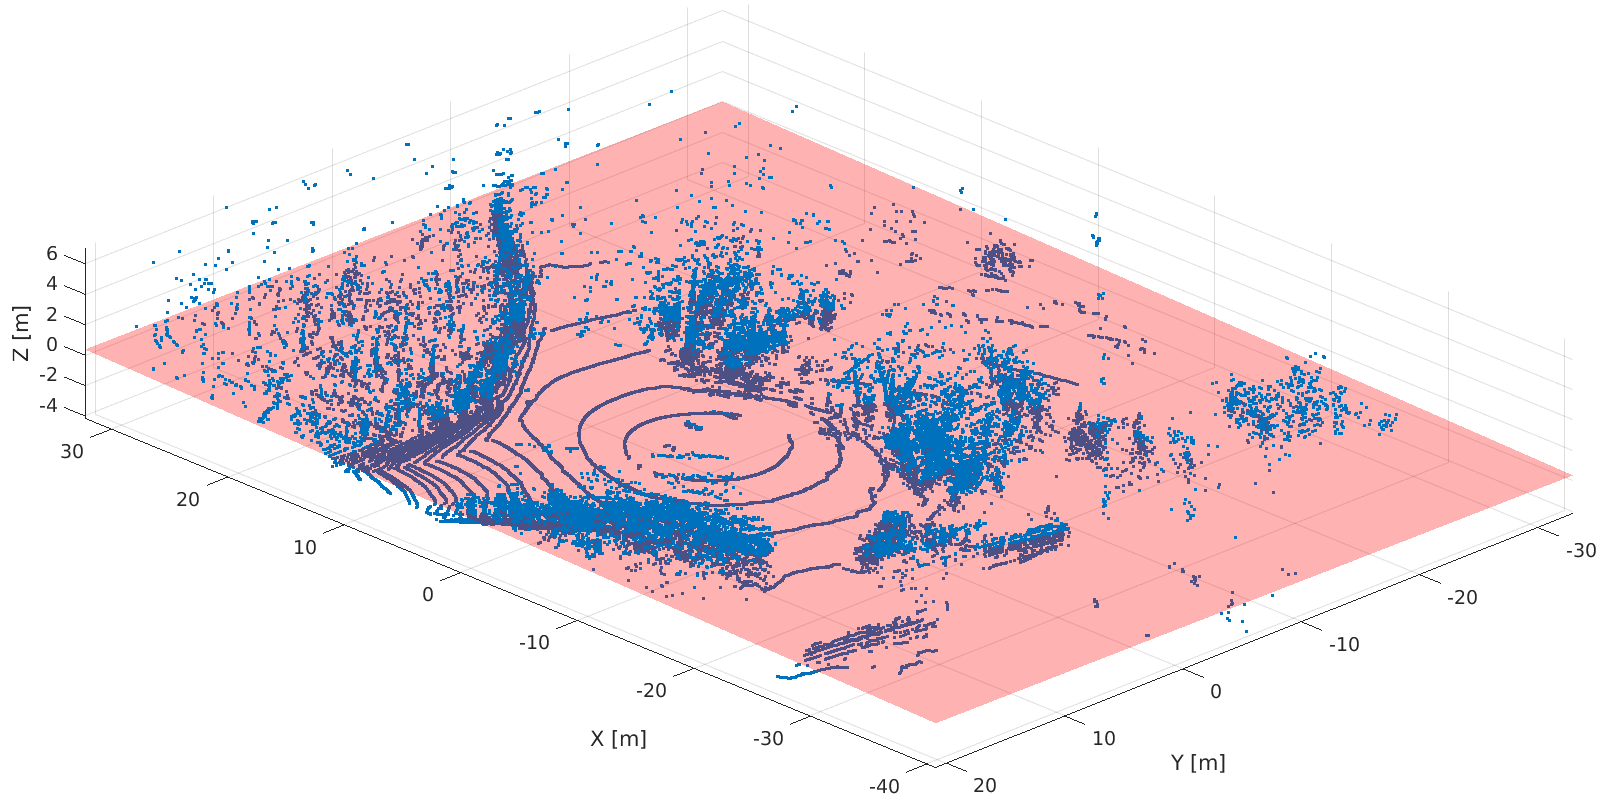
\includegraphics[width=0.7\linewidth]{Defense_Images/Method_Least_Squares_Plane_Proj.png}
			\caption[Method of Least Squares Plane Projection Example]{Method of Least Squares was used to project a plane unto point cloud data.}
			\label{fig:Method_Least_Squares_Plane_Proj}
		\end{figure}
		
	} % End Method of Least Squares Planar Fit
	
	\section{Random Sample Consensus (RANSAC)}{
	
		{RANSAC is an iterative algorithm that is designed to handle large numbers of outliers in the sample data set \cite{derpanis_overview_nodate,yaniv_random_2010,fischler_random_1987,cantzler_random_nodate}, and may be used to fit a two dimensional plane unto a three dimensional point cloud. RANSAC may be described as a two step process that may be repeated until a desired level of accuracy is achieved. First, randomly selected samples from the data set are fitted with a model and the corresponding model parameters are determined. Number of samples corresponds to the desired model, therefore three points will be selected for plane fitting. Second, the entire data set is examined with a cost function to determine consistency with the model. Number of points within the model or inliers is a common method of determining the best estimate \cite{cantzler_random_nodate}. A simplified two dimensional example is shown in Figure \ref{fig:Ransac_2D_Example}. RANSAC model parameters are not generally precise in order to decrease computational load, therefore necessitating a secondary algorithm to analyze a subset of the point cloud. Method of least squares is one such algorithm commonly employed for determining the best fit for the model.}

		\begin{figure}[H]
			\centering
			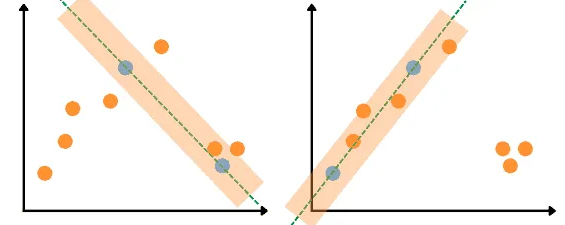
\includegraphics[width=0.7\linewidth]{Defense_Images/RANSAC_good_and_bad.png}
			\caption[2D Simplified RANSAC Example]{Line fitment on a 2d set of points using RANSAC \cite{alam_using_2022}. Poor fitment (left) is shown with minimal number of points within the user-defined threshold area. Better fitment (right) is shown with maximum number of points within the user-defined threshold area.}
			\label{fig:Ransac_2D_Example}
		\end{figure}

		{While RANSAC provides a robust estimation for model parameters, the primary disadvantage is potentially high computationally load \cite{yaniv_random_2010}. Computational efficiency was increased by altering the parameters to allow a more lax fit of the model. Restricting the number of iterations decreased the likelihood of having the best fit while decreasing the computation time.}
	
		{MATLAB's $pcfitplane$ was able to project a plane unto point cloud data gathered from the VLP-32C LiDAR (Figure \ref{fig:RANSAC_example_proj}).}
		
		\begin{figure}[H]
			\centering
			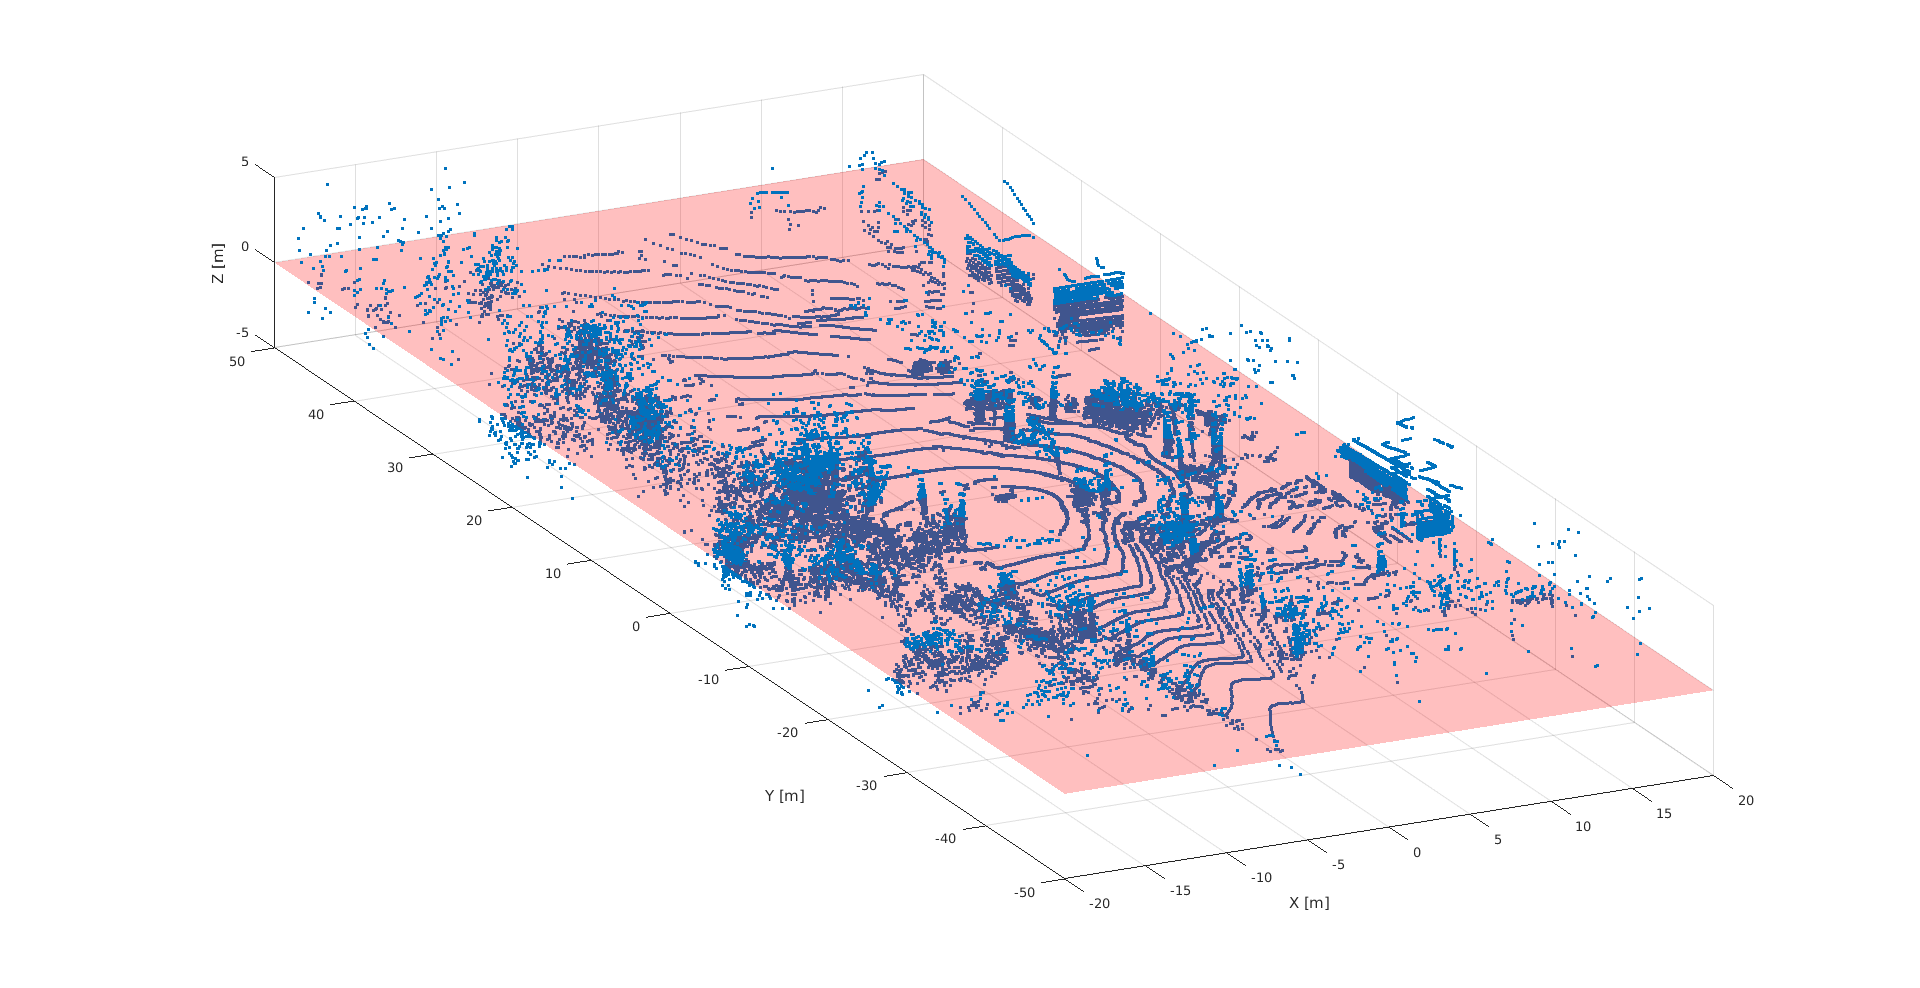
\includegraphics[width=0.7\linewidth]{Defense_Images/RANSAC_example_proj.png}
			\caption[RANSAC Plane Projection Example]{RANSAC plane projection over a point cloud gathered from the VLP-32C Scanning LiDAR.}
			\label{fig:RANSAC_example_proj}
		\end{figure}
		
	} % End RANSAC
	
	\section{Shapiro-Wilks}{
		
		{Testing LiDAR data for normality was completed to determine the usefulness of normality as a feature. Shapiro-Wilk analysis \cite{shapiro_analysis_1965, royston_extension_1982} tests the null hypothesis that a sample vector comes from a normally distributed population, using the test statistic in equation \ref{eq:shapiro_wilks}.}
		
		\begin{equation}
			W = (\sum_{i=1}^{n} a_i x_{(i)})^2 / \sum_{i=1}^{n}(x_i - x_m)^2
			\label{eq:shapiro_wilks}
		\end{equation}
	
		{where $x_i$ is the $i_{th}$ order statistic and $x_m$ is the sample mean \cite{shapiro_analysis_1965}. Coefficients $a_{i}$ are given by equation \ref{eq:shapiro_wilks_coeff}.}
		
		\begin{equation}
			(a_1, a_2, ...,a_n) = m^{T} V^{-1} / C
			\label{eq:shapiro_wilks_coeff}
		\end{equation}
		
		{where C is a vector norm in equation \ref{eq:shapiro_wilks_vector_norm} \cite{davis_covariance_1977}.}
		
		\begin{equation}
			C = |mV^{-1}| = (m^{T} V^{-1} V^{-1} m)^{1/2}
			\label{eq:shapiro_wilks_vector_norm}
		\end{equation}
		
		{where $m$ is the vector of expected values in the normal order statistics: $m = (m_1, m_2,...,m_n)^{T}$ and $V$ is the covariance matrix of the normal order statistics. Shapiro-Wilks was used to test the variance of LiDAR spatial and remission data for normality.}
		
		{MATLAB does not come equipped with a Shapiro-Wilks library, however one was sourced from the MathWorks File Exchange \cite{noauthor_shapiro-wilk_nodate}. Tests for normality against various reference points was completed as an included feature in training a Random Decision Forest algorithm.}	
		
	} % End Shapiro Wilks
	
	\section{Random Decision Forests (RDF)}\label{RDF_SECT}{
		
		{Random Decision Forests is a supervised machine learning method that operates on a set of decision trees \cite{ho_random_1995}. Random Decision Forests have been shown to be useful with handling LiDAR data sets \cite{breiman_random_2001}, and have been employed in terrain classification \cite{laible_3d_2012,laible_map_building,laible_terrain_2013,khan_high_2011,reymann_improving_2015,schilling_geometric_2017, wietrzykowski_context-aware_2019}. Multiple decision trees are created with bootstrapped data sets - randomly selected data sub-sets from a training set. Classification may be determined by the majority results as opposed to the mean \cite{breiman_random_2001,ho_random_1995}. Random Decision Forests may be used to predict road surface area by detecting gravel terrain. Three data bases are conventionally used to train and develop a machine learning algorithm: Training, Testing, and Verification. Training data is the data set from which the Random Decision Forest trains. Training data sets must have roughly equal number of each class to avoid over-training. Training with uneven amounts of data per class type tends to over-classify data as the majority class. Sufficiently large training data sets is necessary to avoid over-training the algorithm to the training data set. Training with a smaller training data set tends to train the algorithm to miss-classify data that does not precisely match the training data set. Testing data is a data set that is independent of the training data but is roughly similar to the training data set. Random Decision Forests do not require a testing data set, as training data is bootstrapped from a larger data set and training data that is not selected may be used as the testing data set. Verification or validation data sets are used to provide an unbiased evaluation of the model by providing data that is non-negligibly dissimilar to the training to testing data sets. }
		
		{MATLAB provides tree ensemble creation functionality using the $TreeBagger$ library. $TreeBagger$ allows for multiple input arguments effecting the resulting Random Decision Forest. Shown in the following code segment is the input arguments used in creating the RDF for this work.}

		\lstinputlisting[style=Matlab-editor, basicstyle=\mlttfamily\scriptsize, caption={TreeBagger function and used input arguments}]{tree_bagger_example.m}

		{Number of trees in the RDF may be defined by $NumTrees$. Number of trees may increase accuracy at the expense of computational efficiency. Accuracy versus number of trees may be tested by calculating out-of-bag and validation error. Training data is given in a table $Training\_Data$ containing all extracted data features. Training data tables must have appropriate headers containing names of used features, but does not contain the class labels. Class labels must be inserted separately, shown in the code block above as $Terrain\_Types$. Class labels must have the same number of rows as the training data table, with each row corresponding to the class that results in the feature values. Table \ref{tab:Training_Data_Example} gives a simplified example of proper formatting of class labels and training data. Maximum number of binary decision splits may be defined in $MaxNumSplits$. Number of bagged features to pull for each individual tree may be defined in $NumPredictorsToSample$. This work followed convention by defining $NumPredictorsToSample$ as the square root of the total number of features. $OOBPredictorImportance$ may be set to $on$ to indicate the storage of out-of-bag estimates of feature importance in the resulting RDF. While this does not effect the resulting RDF, it does serve as a useful post-evaluation tool. $OOBPrediction$ may be defined as $on$ to indicate the storage of out-of-bag information in the RDF. While this does not effect the resulting RDF, it does serve as a useful post-evaluation tool, while eliminating the need to build a separate testing data base. $InBagFraction$ defines the fraction of input data to sample with replacement from the training data set. }

		\begin{table}[H]
			\centering
				\begin{tabular}{ >{\centering}p{3.0cm} >{\centering}p{0.25cm} >{\centering}p{1.5cm} >{\centering}p{1.5cm} >{\centering}p{1.5cm} }
				\textbf{Terrain Types}                       	&                       & \multicolumn{3}{c}{\textbf{Training Data}}                                                                         \tabularnewline \cline{1-1} \cline{3-5} 
				\multicolumn{1}{|c|}{\textit{Classification}} 	& \multicolumn{1}{c|}{} & \multicolumn{1}{c|}{\textit{Feat 1}} & \multicolumn{1}{c|}{\textit{Feat 2}} & \multicolumn{1}{c|}{\textit{Feat 3}} \tabularnewline \cline{1-1} \cline{3-5} 
				\multicolumn{1}{|c|}{gravel}                  	& \multicolumn{1}{c|}{} & \multicolumn{1}{c|}{1}               & \multicolumn{1}{c|}{2}               & \multicolumn{1}{c|}{3}               \tabularnewline \cline{1-1} \cline{3-5} 
				\multicolumn{1}{|c|}{chipseal}                	& \multicolumn{1}{c|}{} & \multicolumn{1}{c|}{4}               & \multicolumn{1}{c|}{5}               & \multicolumn{1}{c|}{6}               \tabularnewline \cline{1-1} \cline{3-5} 
			\end{tabular}
			\caption[TreeBagger Input Argument Example]{Simple example of class label table and training data table.}
			\label{tab:Training_Data_Example}
		\end{table}
		
		{MATLAB was used to predict the terrain type of scanning LiDAR data using the $predict$ function, which requires the RDF and the data that is to be tested. Data to be tested was put into table format, as feature column order (Table \ref{tab:Training_Data_Example}) does not matter, and any additional columns that the RDF was not trained on is ignored.}
		
		\lstinputlisting[style=Matlab-editor, basicstyle=\mlttfamily\scriptsize, caption={Predict function example with intput and output arguments}]{y_fit_example.m}
		
		{Class prediction is yielded in $Yfit$. Scores for each class type in percent probability is given in $scores$, of which the highest score dictates $Yfit$. Standard deviations of predicted classification is given in $stdevs$. For this work, only $Yfit$ was used for testing. Future work may include incorporating all class scores and standard deviations for a more detailed analysis of scanning LiDAR data.}
		
		
	} % End RDF
	
	\section{Closing Statements on Related Work}{
		
		{Current road detection models principally rely upon preexisting geometric or visible features. Localization may be completed by comparing a point cloud of a vehicle's local area to a previously built map of the area using Iterative Closest Point. Neither method may suffice for rural environments, where generalized road features do not exist or the creation of maps would be considered impracticable due to storage constraints. LiDAR has been shown to perform successful terrain classification, and may be able to determine road surface area. Regression analysis may be completed with Method of Least-Squares or a RANSAC based method in order to project a plane unto a point cloud, which will serve as a baseline for examining point cloud spatial properties. .Random Decision Forest Classification is an established method for LiDAR-based terrain classification using machine learning.}
		
	} % End Closing Statements
	
} % End Literature Review

\chapter{Methodology}

{
	
	\subsection{Overview}
	
		{Followed methodology to accomplish this work is outlined in Fig. \ref{fig:flowz_2}. The experimental apparatus for this work was the Ohio University Autonomous Van van (Fig. \ref{fig:Experimental_Apperatus}), which has a Velodyne VLP-32C scanning LiDAR sensor, Novatel PwrPak 7D-E2 GNSS and INS system, and Mako cameras. Raw data was gathered using the Robotic Operating System (ROS) to package incoming scanning LiDAR, GNSS, IMU, and camera sensor data as rosbags. Rosbags were unpacked using MATLAB tools to separate data streams. Prior to creating a training database, manual dictation of gravel and asphalt areas of the gathered point cloud data is necessary. In order to do so, all scanning LiDAR data from a rosbag was aggregated in order to create a single point cloud map. Scanning LiDAR timestamps were matched to the closest GNSS and IMU timestamp data. Closest matching GNSS and IMU data informed the location and orientation of the LiDAR scan (Fig. \ref{fig:road_areas_annotated_22}). Compiled point cloud maps was examined and compared to camera and satellite data to determine gravel and asphalt surface location. Manually defined 2D areas representing gravel and asphalt were projected unto the point cloud (Fig. \ref{fig:road_areas_annotated_22}).}
		
		{Training data was extracted from a single arc from each 360 degree LiDAR scan if the arc was coincident to a manually projected 2D area. Raw spatial and intensity values from the coincident arc were saved to a raw training database. Separate training data bases were maintained for each individual channel. Features that describe the raw spatial and intensity data were extracted. Thirty percent of the training data base was randomly selected and set aside as a validation data base. Training data was visually examined for clustering to verify that a Random Decision Forest would be able to be trained (Fig. \ref{fig:training_data_cluster}). It was found that each class generally clustered to a certain range with some overlap, which indicates that a Random Decision Forest may be trained. MATLAB was used to train a Random Decision Forests for each of the three considered channels using Bayesian Optimization to tune tree depth and number of splits. Training continued until a minimum error was reached (Fig. \ref{fig:c2_min_class_error}). Validation of the RDF was then completed using the validation database.}
		
		{Classification of five rosbags with data gathered from a section of road with three intercepting gravel driveways (one of the gravel driveways was the entrance to the source of the gravel training data). Three arcs from three channels were considered for classification - the centers of the arcs were directly in front of the vehicle, and 45 degrees left and right of center, creating nine total areas in a 3x3 grid in front of the van. Following the same process as aggregating point clouds, GNSS and IMU data informed the location and orientation of the arcs in each 360 degree scan. All arcs were then classified as "asphalt", "gravel", or "unknown", and the averaged coordinates of each arc was aggregated into a single, classified point cloud.}
		
		{Manually defined gravel, asphalt, and side-of-road areas were projected onto the classified point cloud then used to determine the accuracy of the terrain classification algorithm. Classified point clouds were manually examined to determine if the location of gravel and asphalt surfaces may be identified visually. If consecutive points from each channel in any direction had two or more matching gravel or asphalt classification and was evenly spaced, a gravel or road surface area was projected. Guessed road surface areas were then compared to actual areas to determine the method's ability at unmarked gravel road discovery, indicating the method's efficiency at detecting intercepting gravel roads.}
		
		\begin{figure}
			\centering
			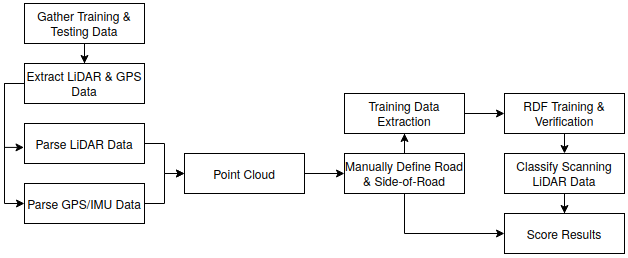
\includegraphics[width=0.7\linewidth]{Defense_Images/flowz_2}
			\caption[Project Flow]{High level view of project work}
			\label{fig:flowz_2}
		\end{figure}
		
		\begin{figure}
			\centering
			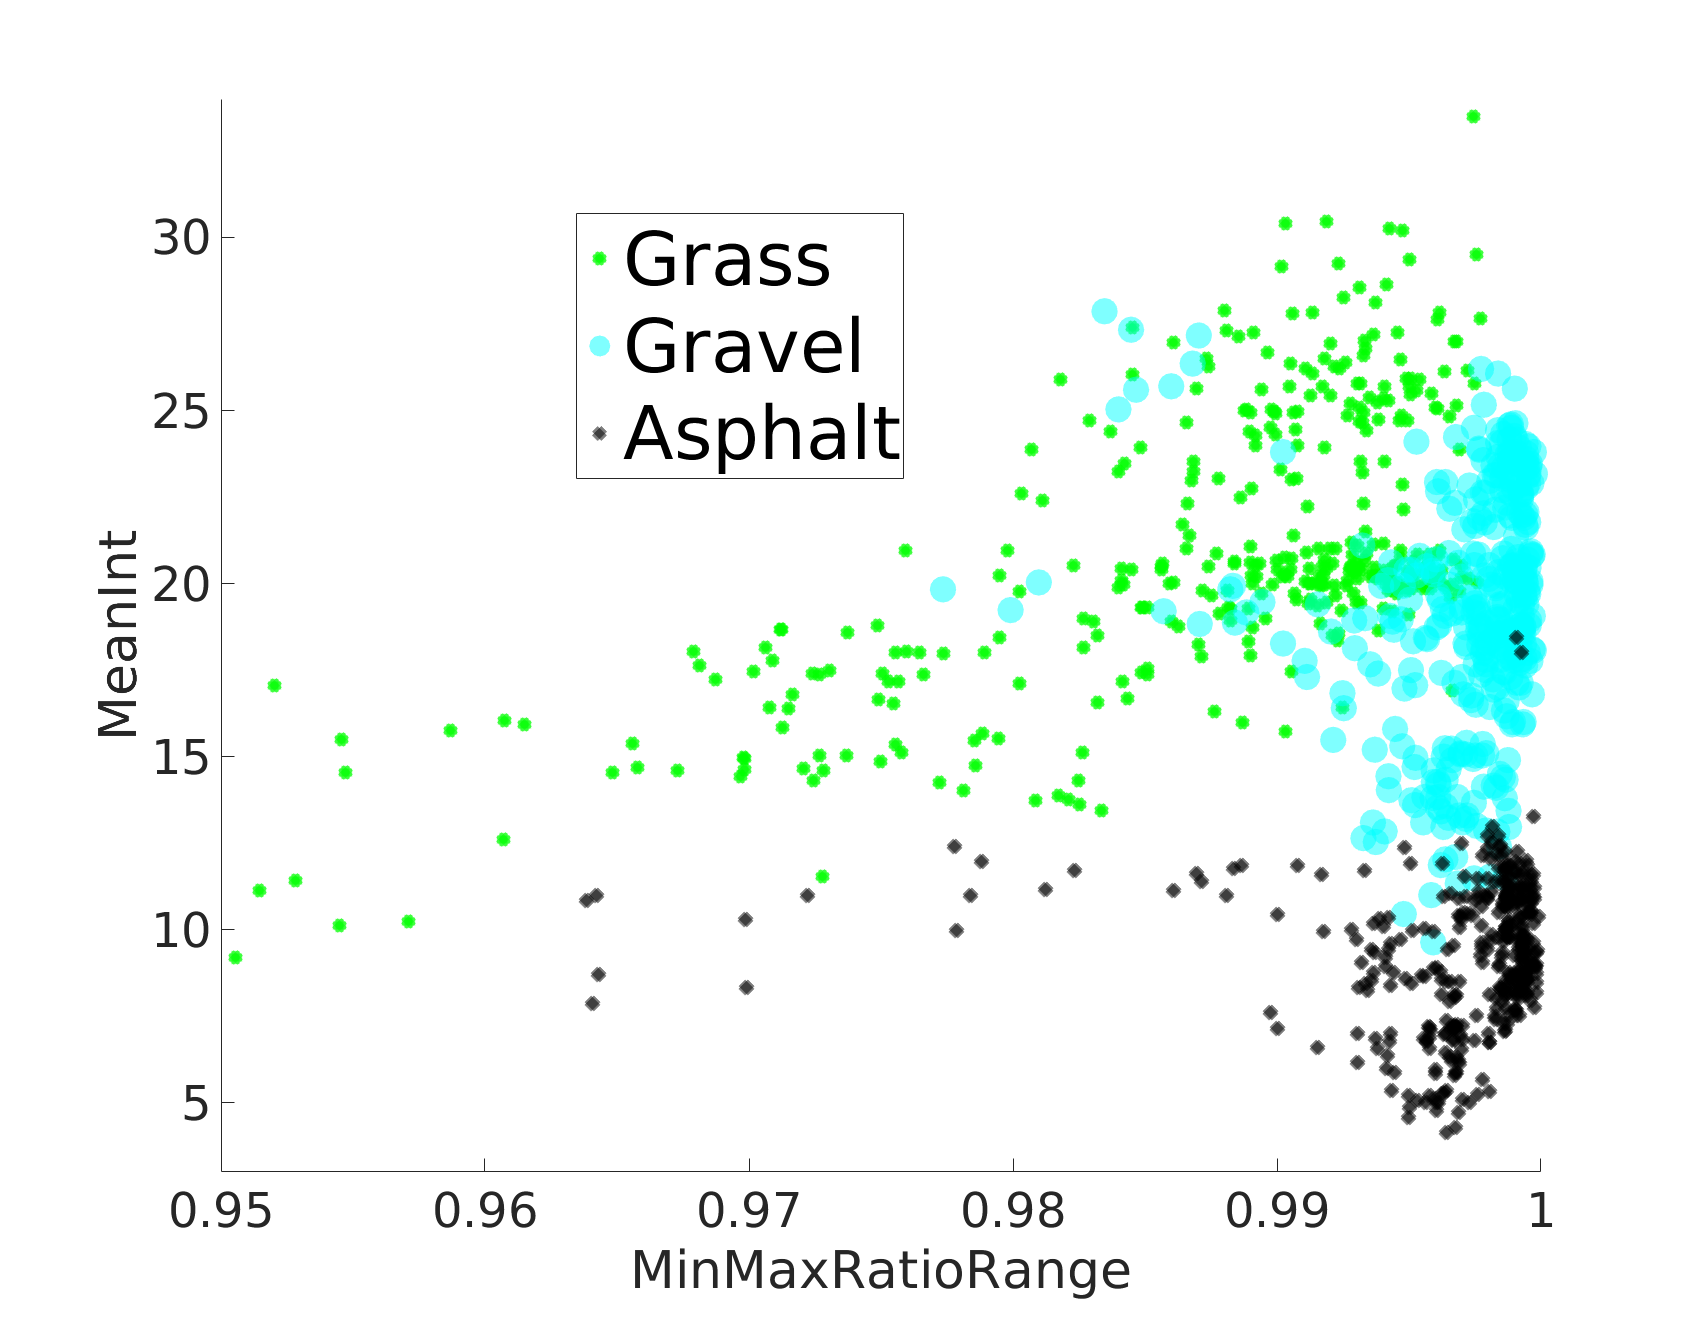
\includegraphics[width=0.7\linewidth]{Defense_Images/training_data_cluster}
			\caption[Example Clustering]{Example of training data comparison between two features.}
			\label{fig:training_data_cluster}
		\end{figure}
		
		\begin{figure}
			\centering
			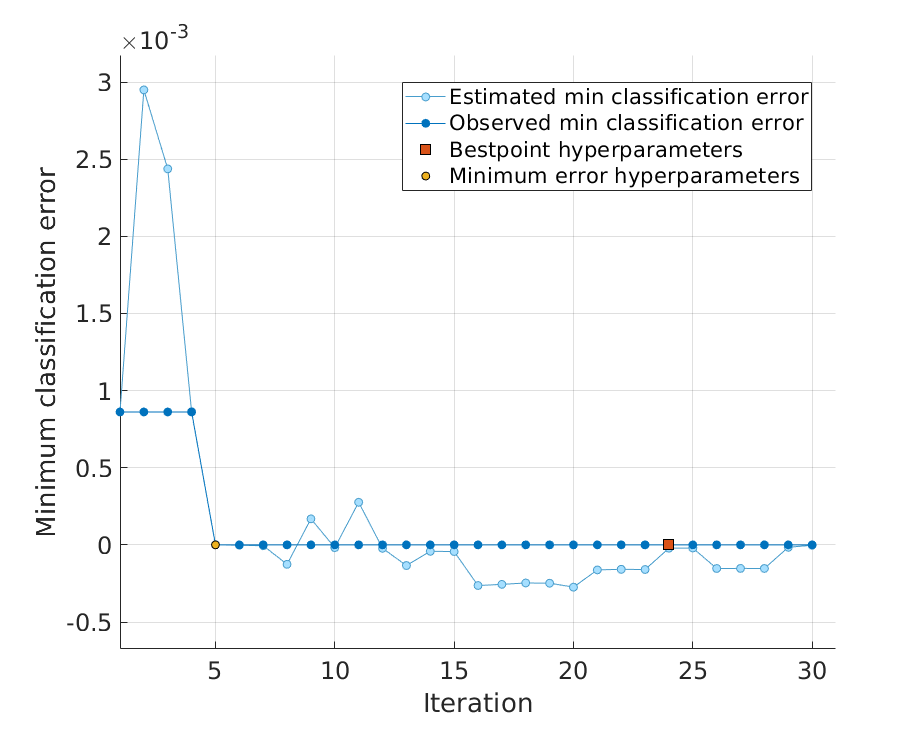
\includegraphics[width=0.7\linewidth]{Defense_Images/c2_min_class_error}
			\caption[RDF Training Classification Error]{Classification error during Bayesian Optimization tuning.}
			\label{fig:c2_min_class_error}
		\end{figure}

	\section{Objective 1}{
		
		{\textbf{Objective Statement: Explore Identify model of adequately describing and simulating a gravel road.} Physical data of a gravel road and a paved road with an intersecting gravel road was gathered using a sensor platform that includes LiDAR and RGB cameras. Regression analysis projection of two dimensional planes using incoming point cloud data to provide a reference point for spacial analysis was explored. Random Decision Forests was explored for classification of a scanning LiDAR spatial and remission data of a gravel road surface. Completion of Objective 1 was accomplished by achieving the goal of gravel road detection. Success was measured by determining the accuracy of detection and the processing time. The outcome of Objective 1 was a method of detecting a physical gravel road with a LiDAR sensor.}
	
		\subsection{Task 1}{
	
			\textbf{Task 1: }{Collect LiDAR and camera data to characterize gravel and paved roads. Data collection took place at a gated gravel lot maintained by Ohio University's Civil Engineering Department as well as public unmarked chipseal and gravel roads near Athens Ohio. Required data was gathered with the Hexegon Chrysler Pacifica New Eagle DBW van. Velodnyne VLP-32C was used to collect physical data of a gravel and paved road surfaces in order to inform a mathematical model describing the road surface. GNSS+INS provided odometer and telemetry data necessary for processing captured point clouds. Incoming sensor data streams was captured by the onboard Linux-based computer. Robotic Operating System's (ROS) interpreted incoming data and exported to a rosbag file for post processing. MATLAB was used to interpret the recorded rosbag and export point cloud and image. }
	
			\subsubsection{Experimental Apparatus Setup}\label{sec:experimental-apparatus-setup}{
		
				{Required physical data was gathered by the Hexegon Chrysler Pacifica New Eagle DBW van (Figure \ref{fig:van}), built by AutonomouStuff, owned and operated by Ohio University. LiDAR point cloud data was gathered with the vehicle's included roof-mounted Velodyne VLP-32C (Figure \ref{fig:vlp32mount}). Velodnyne's VLP-32C has 32 channels producing 300,000 points per second with a vertical field of view from -45$^{\circ}$ to $+$15$^{\circ}$, providing a high output data stream \cite{vlp_32c}. Image data was captured with the forward facing Allied Vision Mako G-319C Cameras equipped with 16 and 12 mm lenses (Figure \ref{fig:makocamera}) producing 2064x1544 px resolution images at 37 Hz. GPS data was recorded by the van's PwrPak7D-E2 GNSS \& INS enclosure manufactured by Novatel equipped with two GNSS-502 antennas manufactured by NavtechGPS.}
					
				\begin{figure}[H]
					\centering
					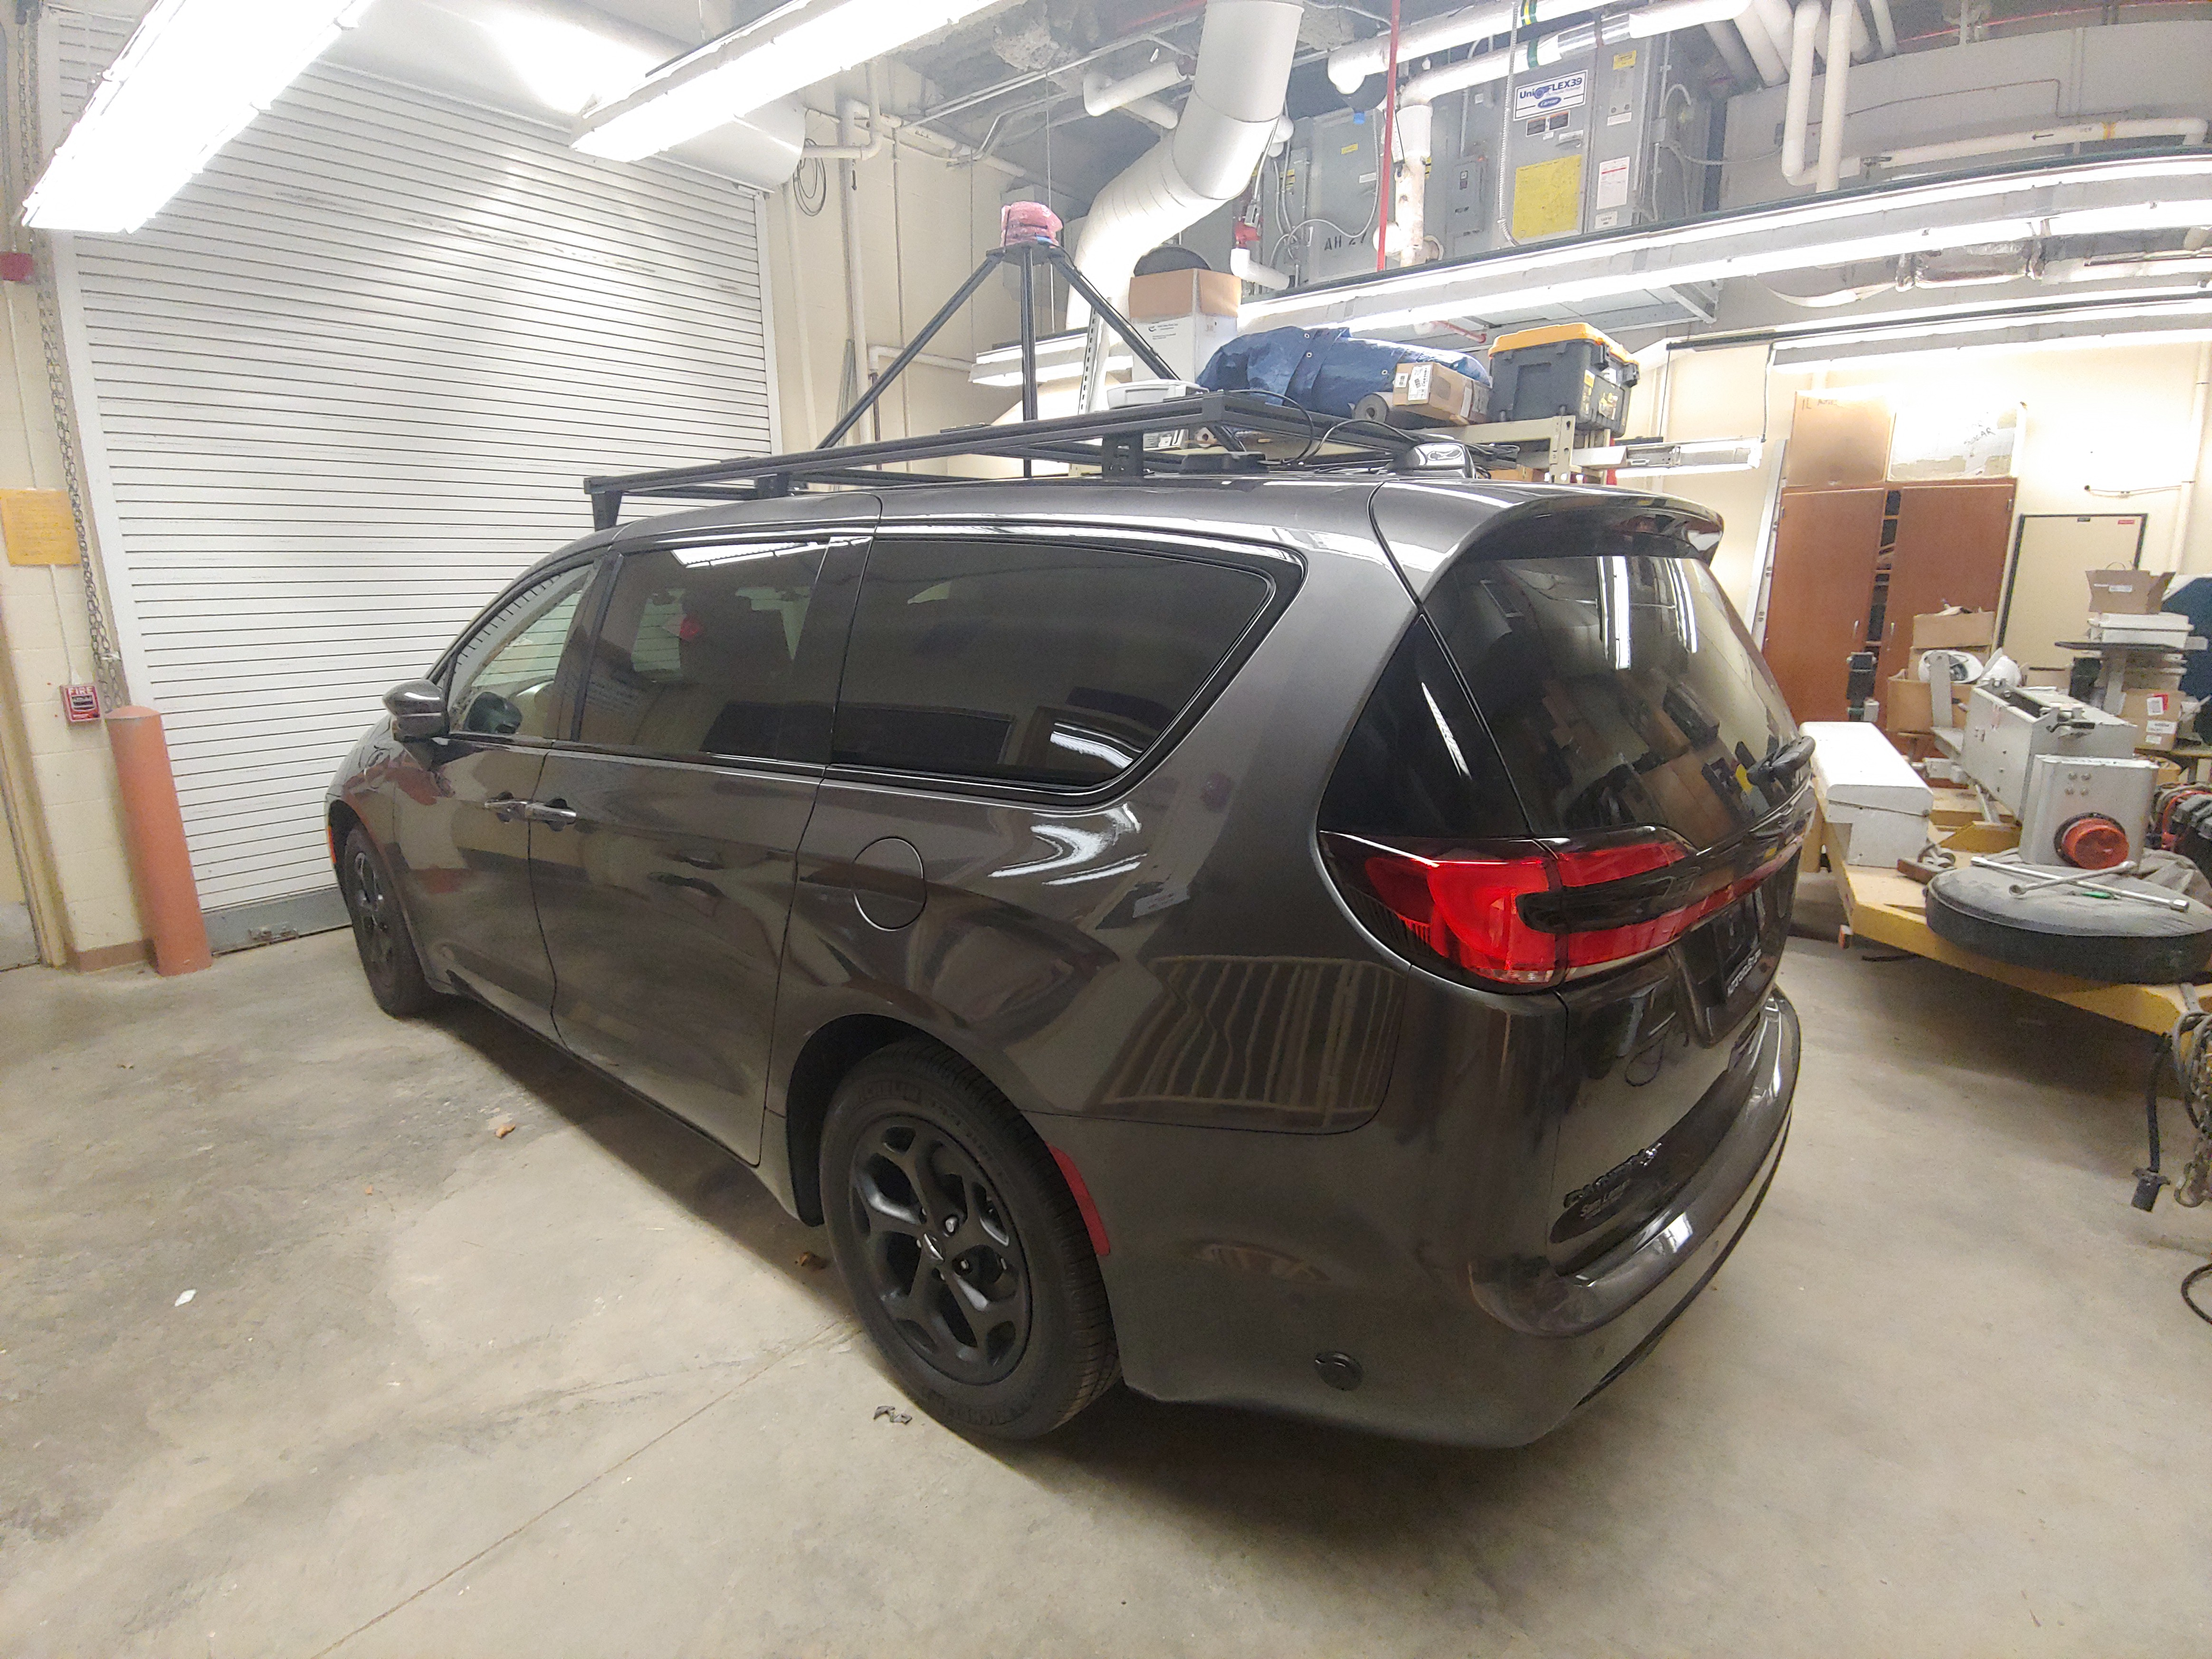
\includegraphics[width=0.7\linewidth]{Defense_Images/Van}
					\caption[Sensor Van]{Sensor Van built by AutonomouStuff}
					\label{fig:van}
				\end{figure}
			
				\begin{figure}[H]
					\centering
					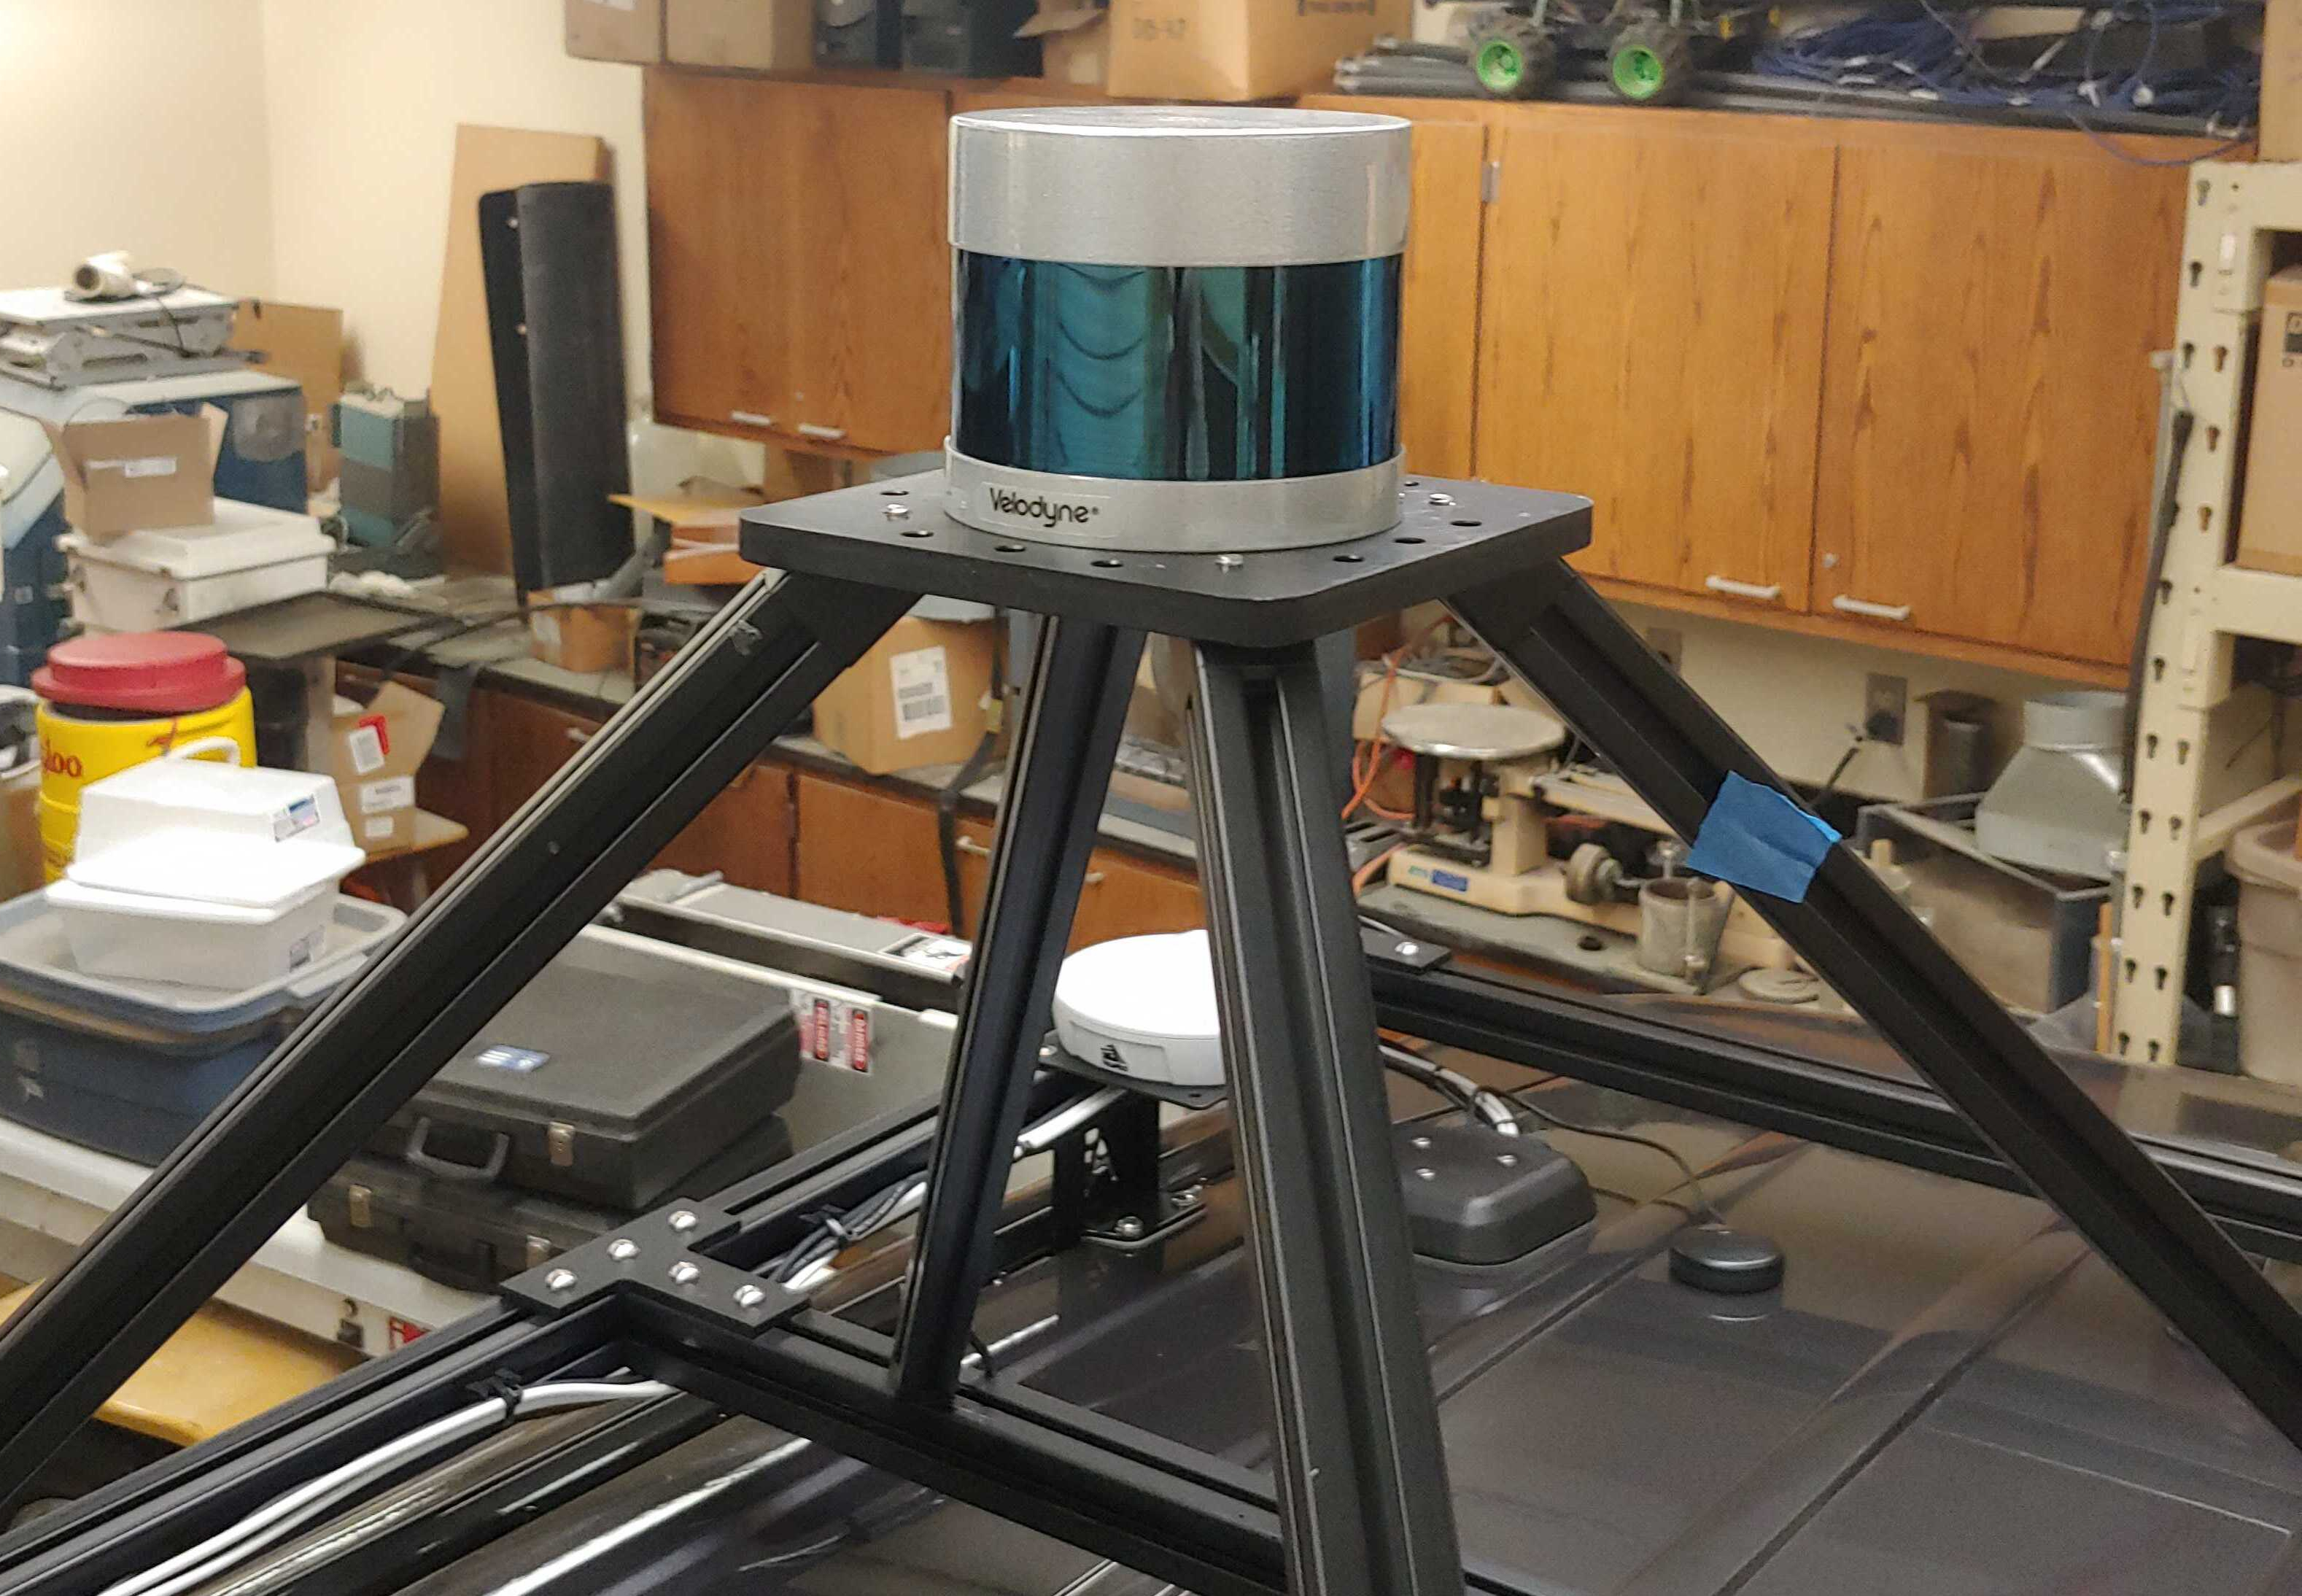
\includegraphics[width=0.7\linewidth]{Defense_Images/vlp_32_mount_2}
					\caption[VLP 32 on Van]{Velodyne's VLP-32 is mounted on top of the Sensor Van.}
					\label{fig:vlp32mount}
				\end{figure}
				
				\begin{figure}[H]
					\centering
					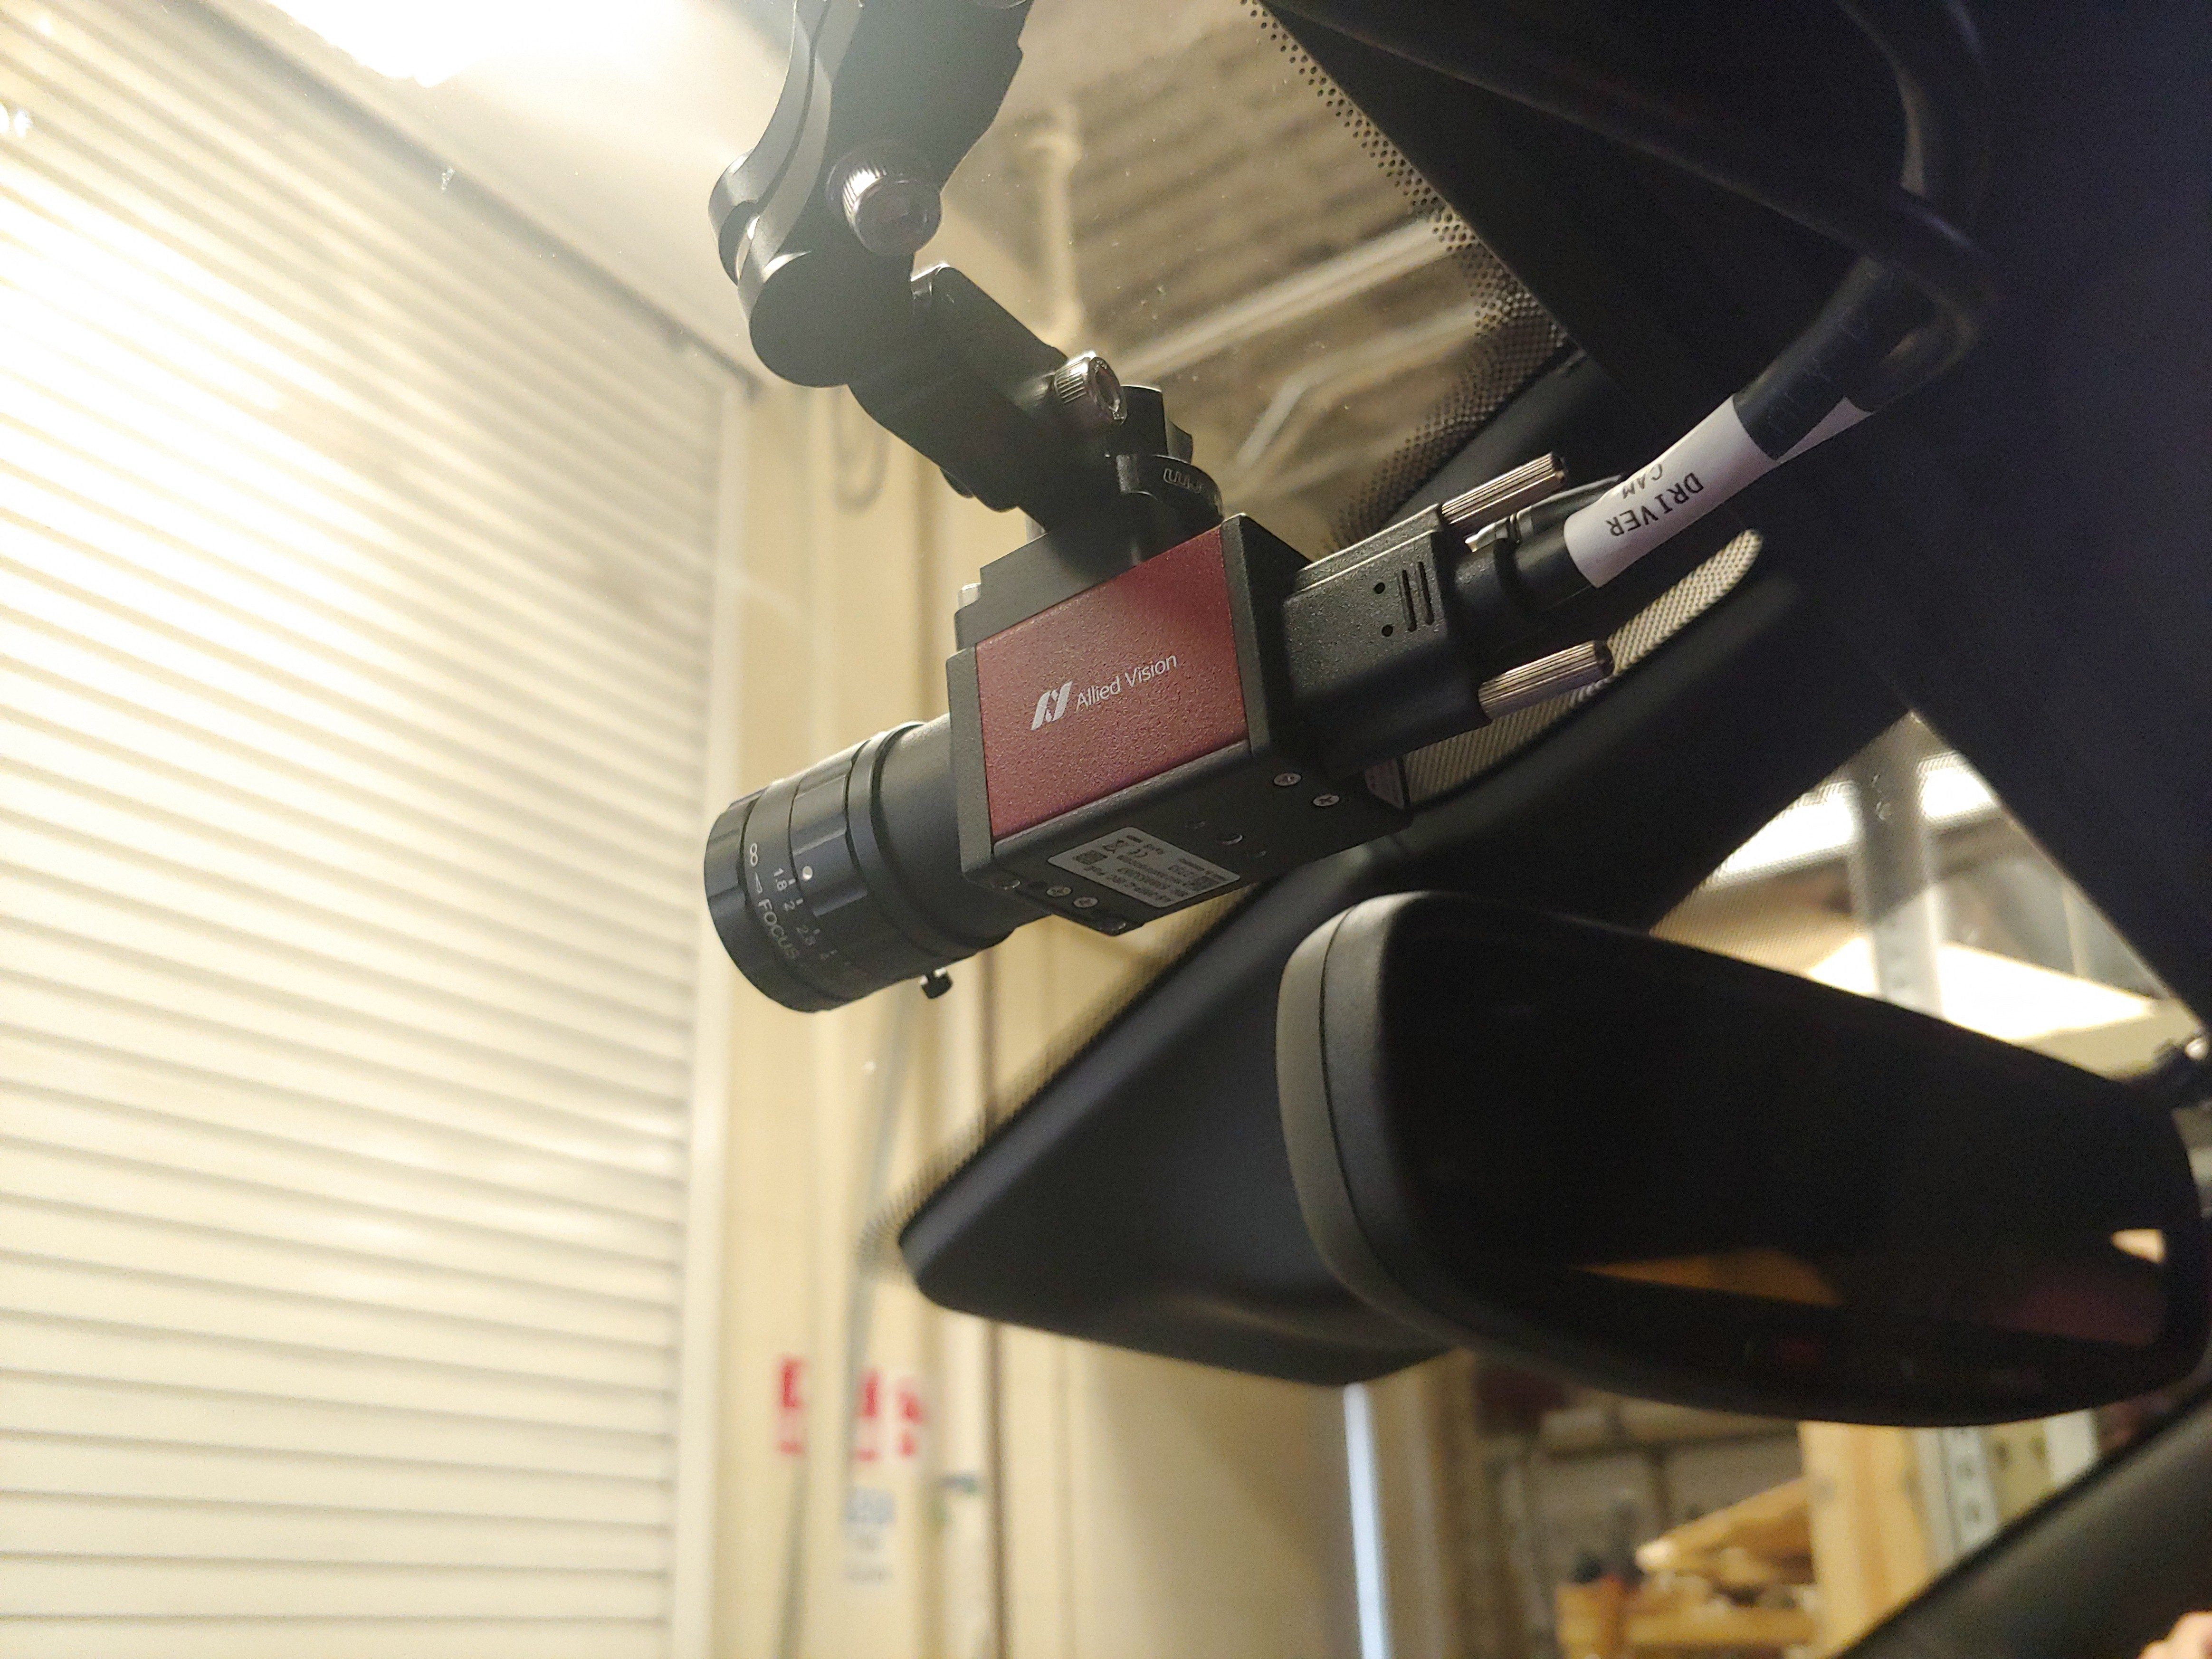
\includegraphics[width=0.7\linewidth]{Defense_Images/Mako_Camera}
					\caption[Mako Camera]{One of the two forward facing Mako Cameras in the van}
					\label{fig:makocamera}
				\end{figure}
			
			}
			
			\subsubsection{Data Collection}{
			
				{Scanning LiDAR training data was collected on various roads and lots near Athens, Ohio. Scanning LiDAR data of gravel surfaces was gathered principally from an un-named gravel road near Armig Road (Figures \ref{fig:Combined_Armig}) and a gravel lot maintained by the Ohio University Civil Engineering Department near Blackburn Road (Figures \ref{fig:Combined_Gravel_Lot}). Additional gravel road data for testing purposes only was gathered on Sturbois Road (Figures \ref{fig:Combined_Sturbois}). Scanning LiDAR data of chipseal surfaces was gathered principally from Bean Hollow Road (Figures \ref{fig:Combined_Bean}). Additional chipseal road data for testing purposes only was gathered on later portions of both Bean Hollow Road. Scanning LiDAR data of grassy surfaces and foliage was gathered from the sides of the previously stated roads, therefore not special data collection drive was made for those terrain types.}
				
				%[width=1.0\linewidth,height=8.0 cm,keepaspectratio]
				
				\begin{figure}[H]
					\centering
					\begin{subfigure}{0.45\textwidth}
						\centering
						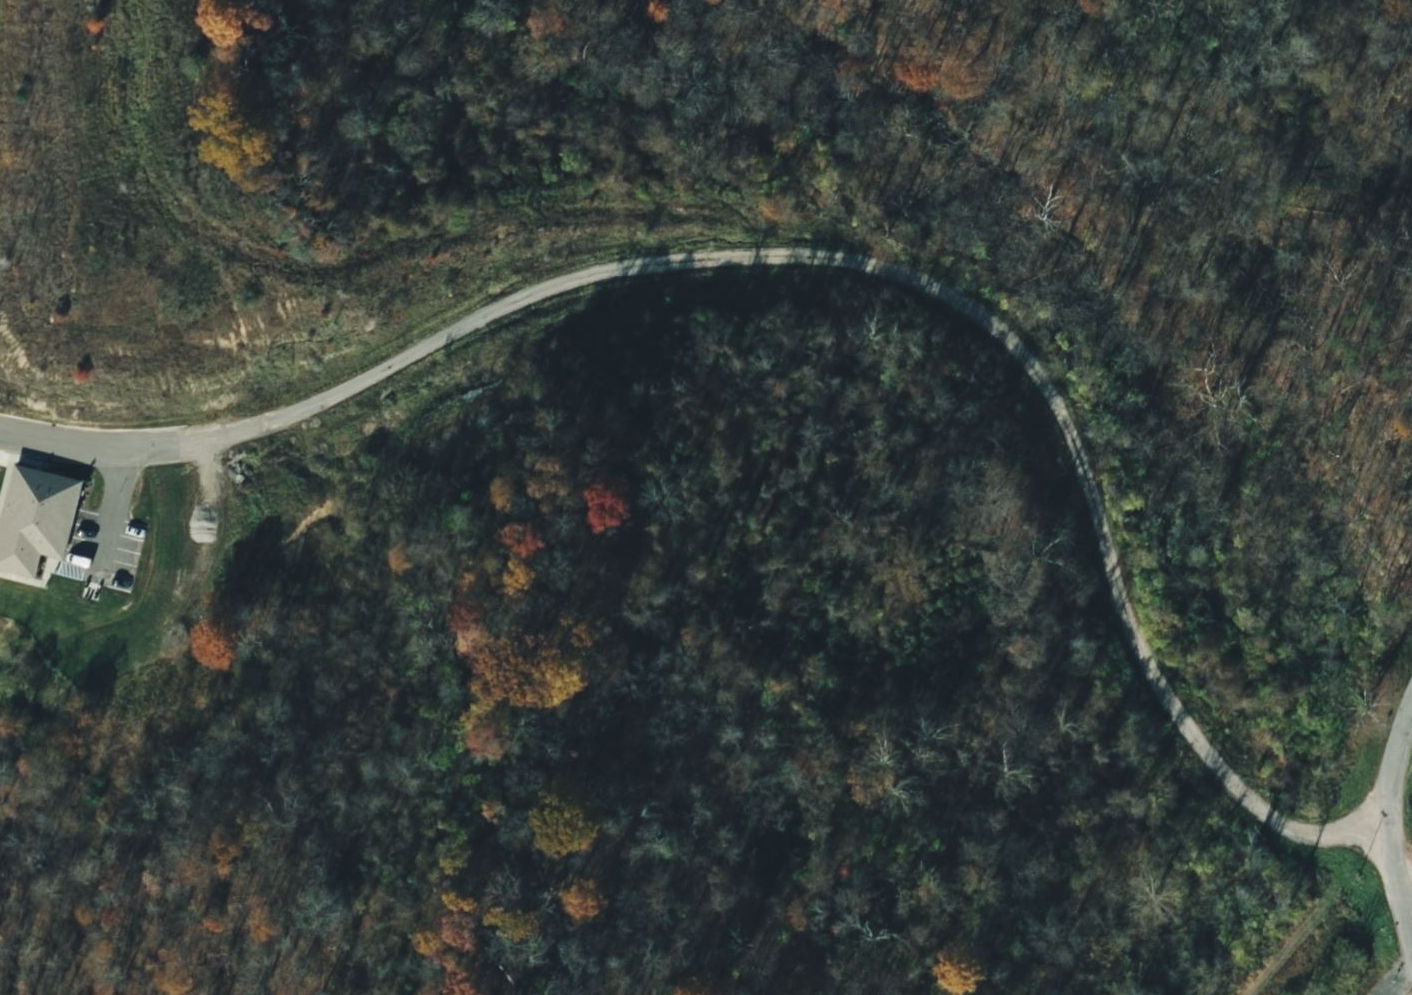
\includegraphics[width=1.0\linewidth,height=5.0 cm,keepaspectratio]{Defense_Images/Gravel_Road_Armig}
						\caption[Armig Road Satellite View]{}
						\label{fig:Armig_Road_Sat_View}
					\end{subfigure}
					\begin{subfigure}{0.45\textwidth}
						\centering
						\includegraphics[width=1.0\linewidth,height=5.0 cm,keepaspectratio]{Defense_Images/armig_2}
						\caption[Armig Road Camera View]{}
						\label{fig:Armig_Road_Camera_View}
					\end{subfigure}
					\caption[Armig Road]{Satellite view of Armig Road (a), Road view of Armig Road (b)}
					\label{fig:Combined_Armig}
				\end{figure}
			
				\begin{figure}[H]
					\centering
					\begin{subfigure}{0.45\textwidth}
						\centering
						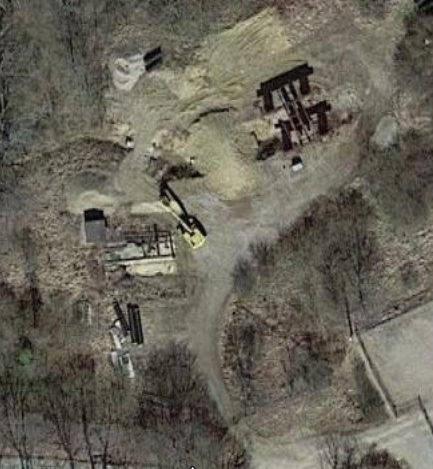
\includegraphics[width=1.0\linewidth,height=5.0 cm,keepaspectratio]{Defense_Images/Gravel_Lot}
						\caption[Gravel Lot Satellite View]{}
						\label{fig:Gravel_Lot_Sat_View}
					\end{subfigure}
					\begin{subfigure}{0.45\textwidth}
						\centering
						\includegraphics[width=1.0\linewidth,height=5.0 cm,keepaspectratio]{Defense_Images/gravel_lot_example}
						\caption[Gravel Lot Camera View]{}
						\label{fig:Gravel_Lot_Camera_View}
					\end{subfigure}
					\caption[Gravel Lot]{Satellite view of the Gravel Lot (a), Road view of the Gravel Lot (b)}
					\label{fig:Combined_Gravel_Lot}
				\end{figure}
			
				\begin{figure}[H]
					\centering
					\begin{subfigure}{0.45\textwidth}
						\centering
						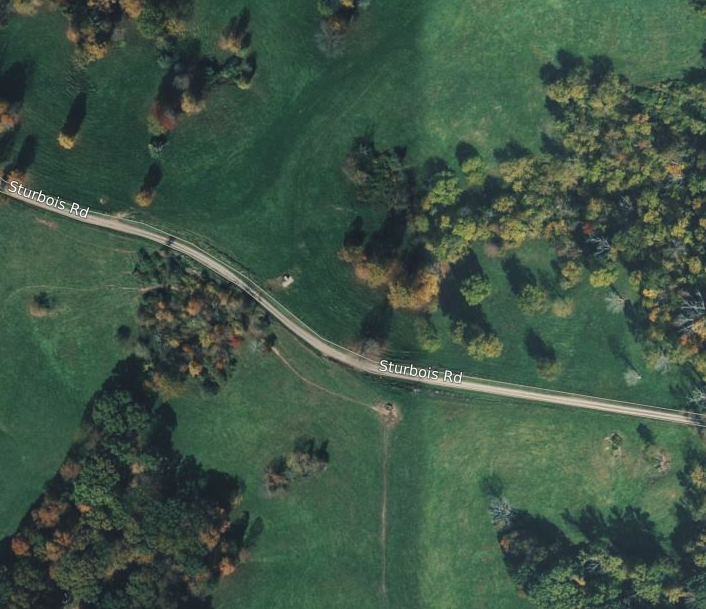
\includegraphics[width=1.0\linewidth,height=5.0 cm,keepaspectratio]{Defense_Images/Sturbois_Road}
						\caption[Sturbois Road Satellite View]{}
						\label{fig:Sturbois_Sat_View}
					\end{subfigure}
					\begin{subfigure}{0.45\textwidth}
						\centering
						\includegraphics[width=1.0\linewidth,height=5.0 cm,keepaspectratio]{Defense_Images/sturbois_1_straight_camera}
						\caption[Sturbois Road Camera View]{}
						\label{fig:Sturbois_Cam_View}
					\end{subfigure}
					\caption[Sturbois Road]{Satellite view of Sturbois Road (a), Road view of Sturbois Road (b)}
					\label{fig:Combined_Sturbois}
				\end{figure}
			
				\begin{figure}[H]
					\centering
					\begin{subfigure}{0.45\textwidth}
						\centering
						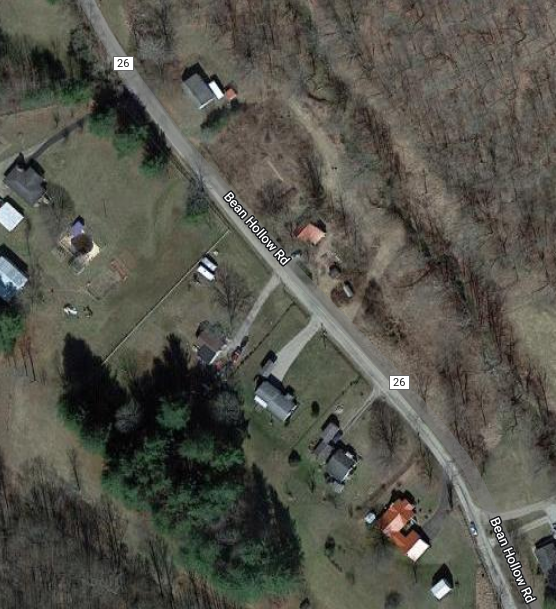
\includegraphics[width=1.0\linewidth,height=5.0 cm,keepaspectratio]{Defense_Images/Bean_Hollow_Road}
						\caption[Bean Hollow Road Satellite View]{}
						\label{fig:Bean_Sat_View}
					\end{subfigure}
					\begin{subfigure}{0.45\textwidth}
						\centering
						\includegraphics[width=1.0\linewidth,height=5.0 cm,keepaspectratio]{Defense_Images/Bean_Hollow_Road_Camera}
						\caption[Bean Hollow Road Camera View]{}
						\label{fig:Bean_Cam_View}
					\end{subfigure}
					\caption[Bean Hollow Road]{Satellite view of Bean Hollow Road (a), Road view of Bean Hollow Road (b)}
					\label{fig:Combined_Bean}
				\end{figure}
						
			} % End Data Collection
				
			\subsubsection{Data Processing}\label{sec:data_processing}{

				{MATLAB was used to process the gathered rosbag files using the MATLAB ROSBAG library. Rosbags were directly loaded into the MATLAB environment. Point cloud topic was defined, and the point cloud messages were read from the topic and imported as a data structure. Cartesian coordinates and corresponding intensity values were extracted and saved to disk.}
				
				{GPS and IMU data was extracted in a similar manner. GPS and IMU topics were defined, and topic messages are read. Longitude, latitude, and altitude were extracted from the GPS messages, while roll, pitch, and yaw were extracted from the IMU messages.}
		
			} % End Data Processing
				
		} % End Task 1

		\subsection{Task 2}{

			\textbf{Task 2: }{Analyze point cloud data for determining a mathematical model describing a physical gravel road surface. Point cloud data lying on the gravel road surface was manually isolated using MATLAB by defining areas pertaining to one of the four considered terrain types. Establishment of a ground plane using RANSAC or Method of Least Squares was necessary to provide a point of reference for spacial data analysis. Granular examination of scanning LiDAR spatial and remission data was accomplished by discretizing LiDAR channels into quadrants. Features such as mean, median, and roughness that will be used to characterize scanning LiDAR spatial and remission data. Random Decision Forests was explored as a method of terrain classification using features derived from scanning LiDAR spatial and remission data. Verifying the model was completed by scoring classification accuracy against a  data set with known terrain types.}
			
			\subsubsection{RANSAC and Method of Least Squares Plane Projection}{
				
				{Projection of a plane was necessary to provide a reference point for describing point variance. RANSAC and Method of Least Squares were tested for use as plane projection methods. Alternatively, perpendicular distance from the LiDAR origin was also considered, which has a computational advantage in that it may be read directly from the Velodyne VLP-32 data stream.}
			
				{RANSAC was implementing by a built-in MATLAB function, $pcfitplane$. Method of Least Squares was implemented by importing a MATLAB library \cite{noauthor_object-oriented_nodate}. Comparison of computational efficiency between the two methods was accomplished by creating a script that would load a point cloud file and determine the length of time required to project a plane. Comparisons between validation data set classification accuracy and out-of-bag error were made to gauge the performance between the two plane projection methods.}
			
			} % End RANSAC and Method of Least Squares Plane Projection
	
			\subsubsection{Training and Verification Data Selection Process}\label{sec:training_and_verification_data_selection_process}{
			
%				{Scanning LiDAR training and verification data was gathered from the exported PCD by manually selecting appropriate consecutive points representing gravel, chipseal, foliage, and grass surfaces. A process was later developed where training data was gathered by selecting larger areas in a combined point cloud map (\ref{sec:grab_tform}).}
%					
%				{Point clouds are individually imported into the MATLAB environment. RANSAC or Method of Least Squares may be used to project a reference plane unto the point cloud. Displaying the point cloud is completed using MATLAB's $pcshow$ function. Training data is selected by manually drawing an area around appropriate points of a desired terrain type using MATLAB's $drawrectangle$ function (Figure \ref{fig:Rectangle_ROI}). Indices for the rectangle are extracted, and MATLAB's function $findPointsInROI$ is used to extract any points within the drawn rectangle (Figure \ref{fig:ROI_Points}). Captured points are then saved to disk along with the projected plane's normal vector and distance from the origin $[a,b,c,d]$.}
%				
%				\begin{figure}[H]
%					\centering
%					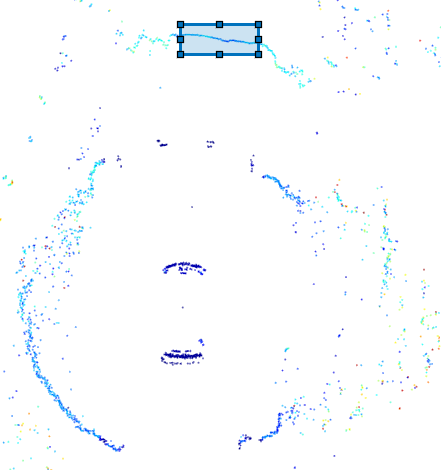
\includegraphics[width=0.5\linewidth]{Defense_Images/Rectangle_ROI}
%					\caption[Region of Interest Selection]{MATLAB was used to select training data using the $drawrectangle$ function and extracting points that lay within the defined area.}
%					\label{fig:Rectangle_ROI}
%				\end{figure}
%				
%				\begin{figure}[H]
%					\centering
%					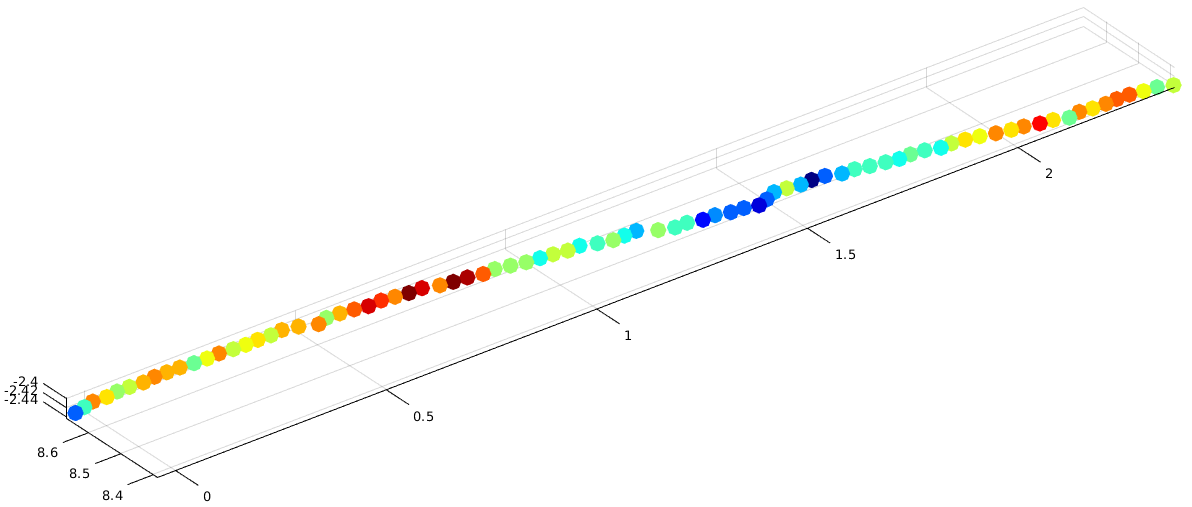
\includegraphics[width=0.5\linewidth]{Defense_Images/ROI_Points}
%					\caption[Points in Region of Interest]{MATLAB was used to select training data using the $drawrectangle$ function and extracting points that lay within the defined area. Shown is an example of the points from that process}
%					\label{fig:ROI_Points}
%				\end{figure}

				{Scanning LiDAR training data was gathered  from rosbags containing scanning LiDAR, GPS, and IMU data in a two step process.  Combined point cloud data was loaded into the MATLAB environment and displayed (Figure \ref{fig:Pre-Manual_Classify_1}). Manually defined areas representing gravel, chipseal, foliage, or grass were created and projected unto the combined point cloud (Figure \ref{fig:Post-Manual_Classify_1}). Consecutive scanning LiDAR points from the source ROSBAG were extracted if sympatric to manually defined areas.}
				
				\begin{figure}[H]
					\centering
					\begin{subfigure}{0.45\textwidth}
						\centering
						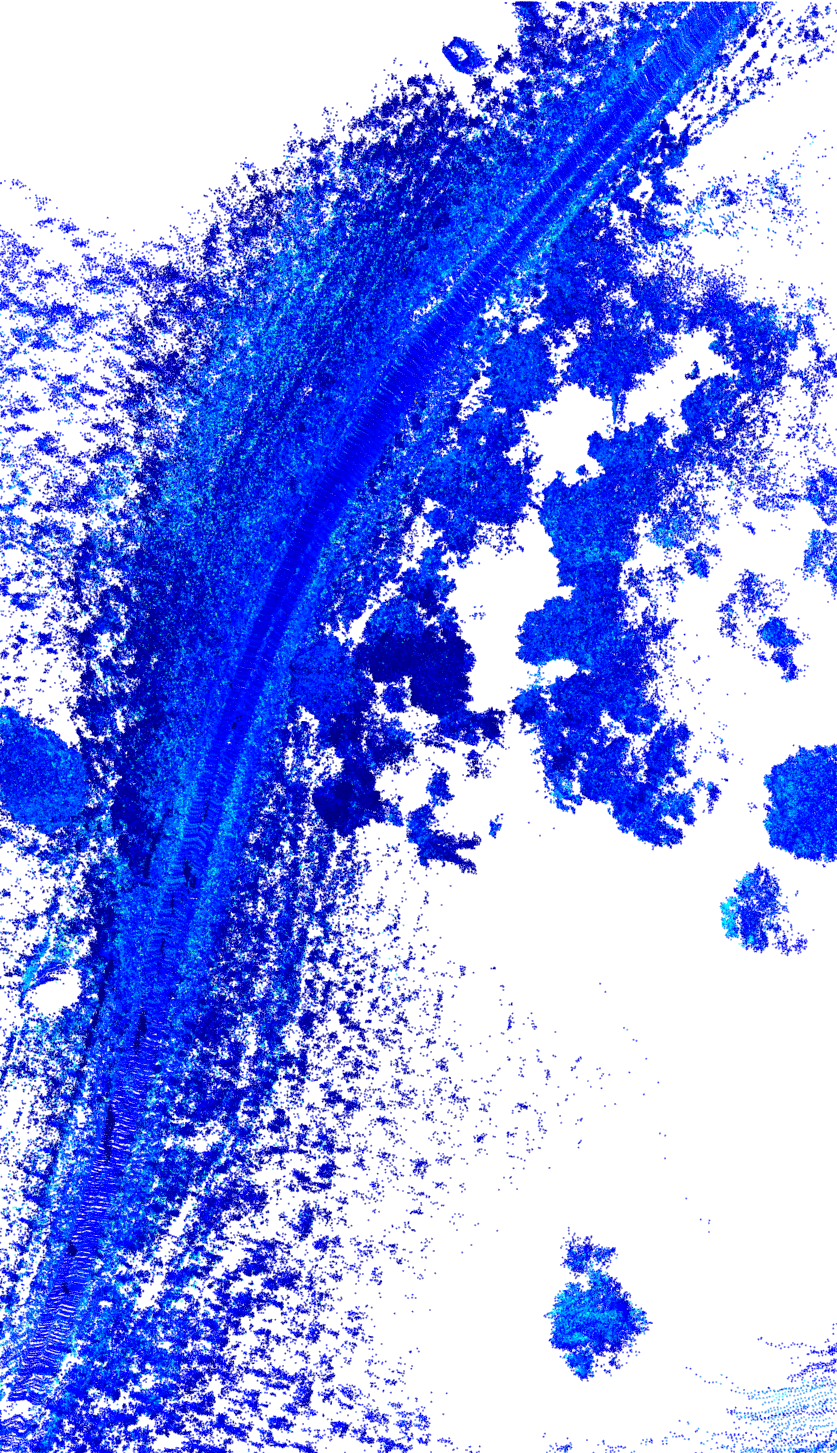
\includegraphics[width=1.0\linewidth]{Defense_Images/Pre-Manual_Classify_1}
						\caption[Bean Hollow Road Satellite View]{}
						\label{fig:Pre-Manual_Classify_1}
					\end{subfigure}
					\begin{subfigure}{0.45\textwidth}
						\centering
						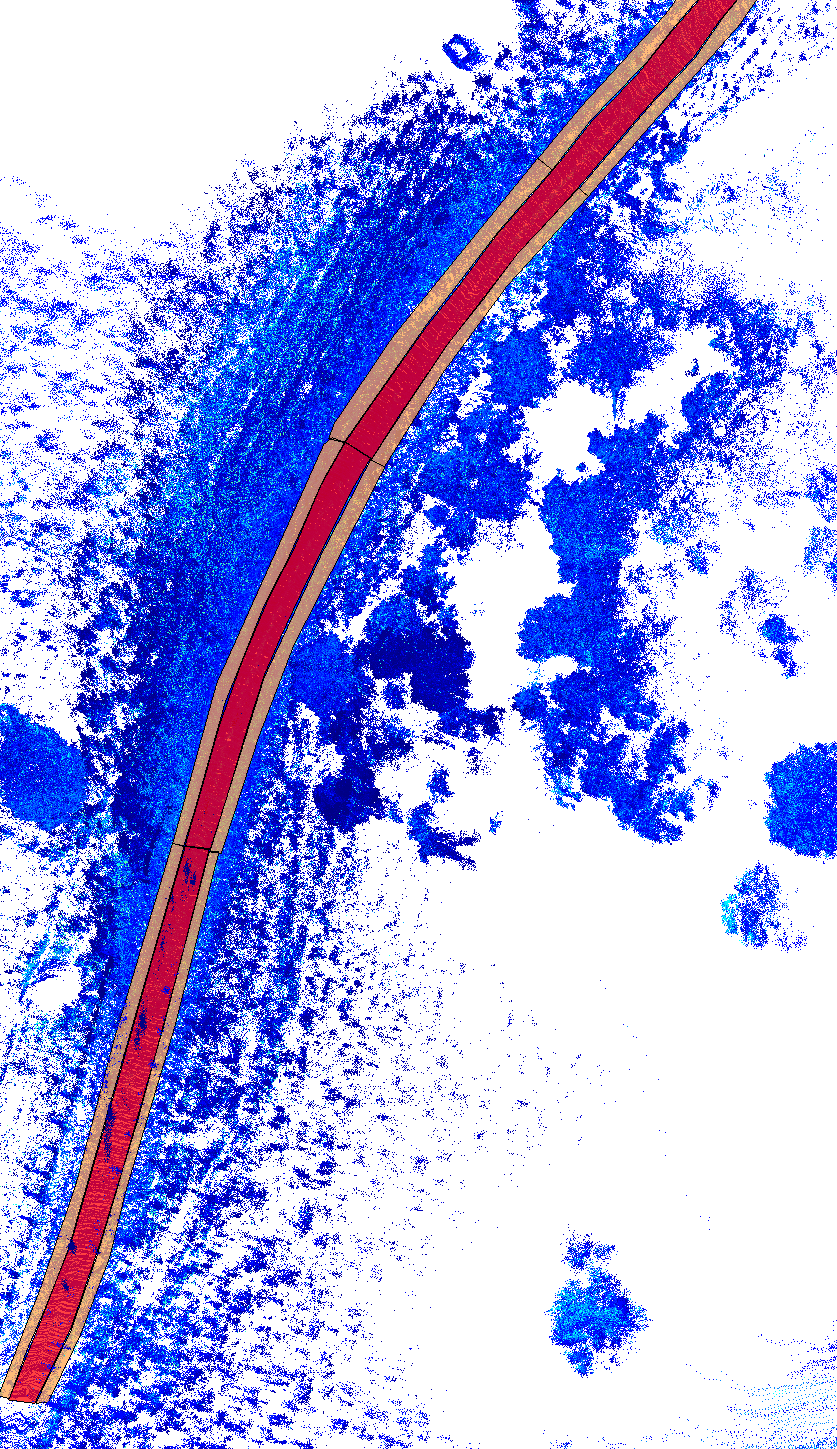
\includegraphics[width=1.0\linewidth]{Defense_Images/Post-Manual_Classify_1}
						\caption[Bean Hollow Road Camera View]{}
						\label{fig:Post-Manual_Classify_1}
					\end{subfigure}
					\caption[Manual Point Cloud Classification Overview]{Top-Down view of a combined point cloud (a). Road surface terrain types may be defined manually (b), in this case as gravel (red). Side-of-road areas may also be defined (orange). }
					\label{fig:Manual_Classification_Overview}
				\end{figure}
				
				{MATLAB's $drawpolygon$ function was used to select an area representing gravel, chipseal, foliage, or grass (Figure \ref{fig:Area_Selection_Process}).}
	
				\begin{figure}[H]
					\centering
					\begin{subfigure}{0.45\textwidth}
						\centering
						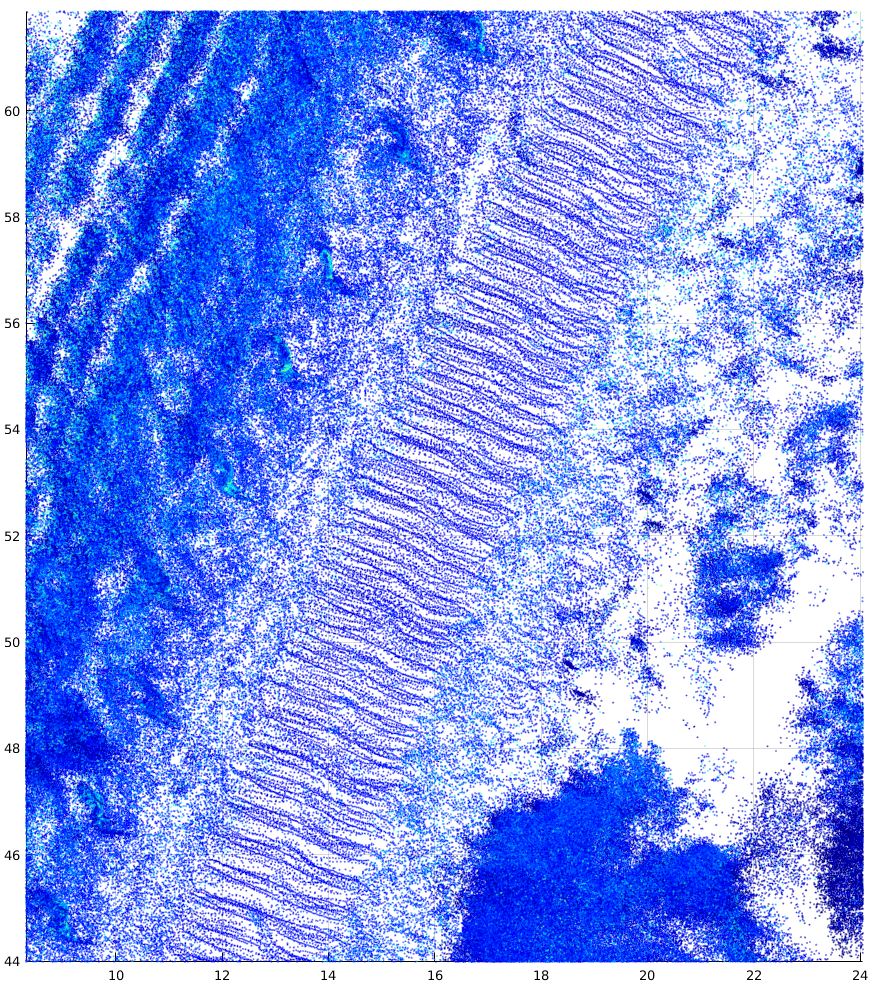
\includegraphics[width=1.0\linewidth]{Defense_Images/pre_select_area}
						\caption[Bean Hollow Road Satellite View]{}
						\label{fig:pre_select_area}
					\end{subfigure}
					\begin{subfigure}{0.45\textwidth}
						\centering
						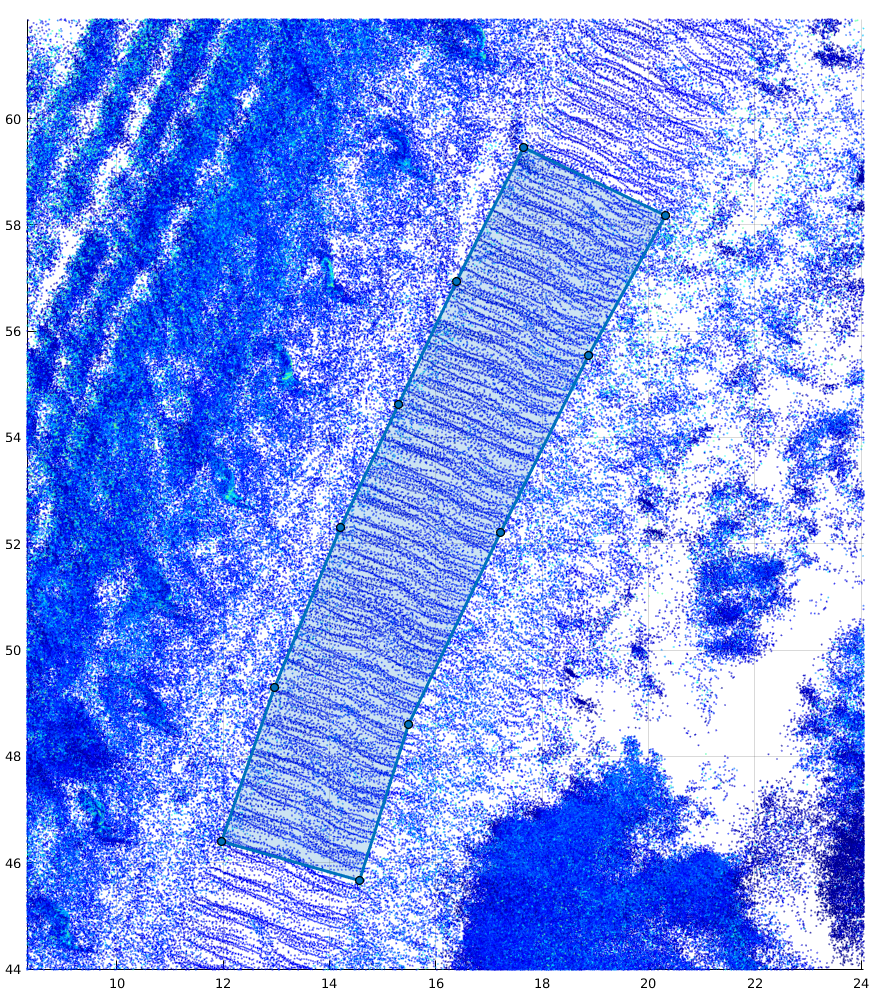
\includegraphics[width=1.0\linewidth]{Defense_Images/area_selected}
						\caption[Bean Hollow Road Camera View]{}
						\label{fig:area_selected}
					\end{subfigure}
					\caption[Manual Area Selection Process]{Combined scanning LiDAR point cloud data (a) may be manually defined using MATLAB's $drawpolygon$ function to select the desired area. }
					\label{fig:Area_Selection_Process}
				\end{figure}
				
				{MATLAB's $inpolygon$ function was used to extract scanning LiDAR data that was sympatric to the manually defined areas. Visual confirmation was made that the extracted points correspond to the desired terrain type. Extracted scanning LiDAR data was then saved to disk in separate .mat files.}
				
				\begin{figure}[H]
					\centering
					\begin{subfigure}{0.45\textwidth}
						\centering
						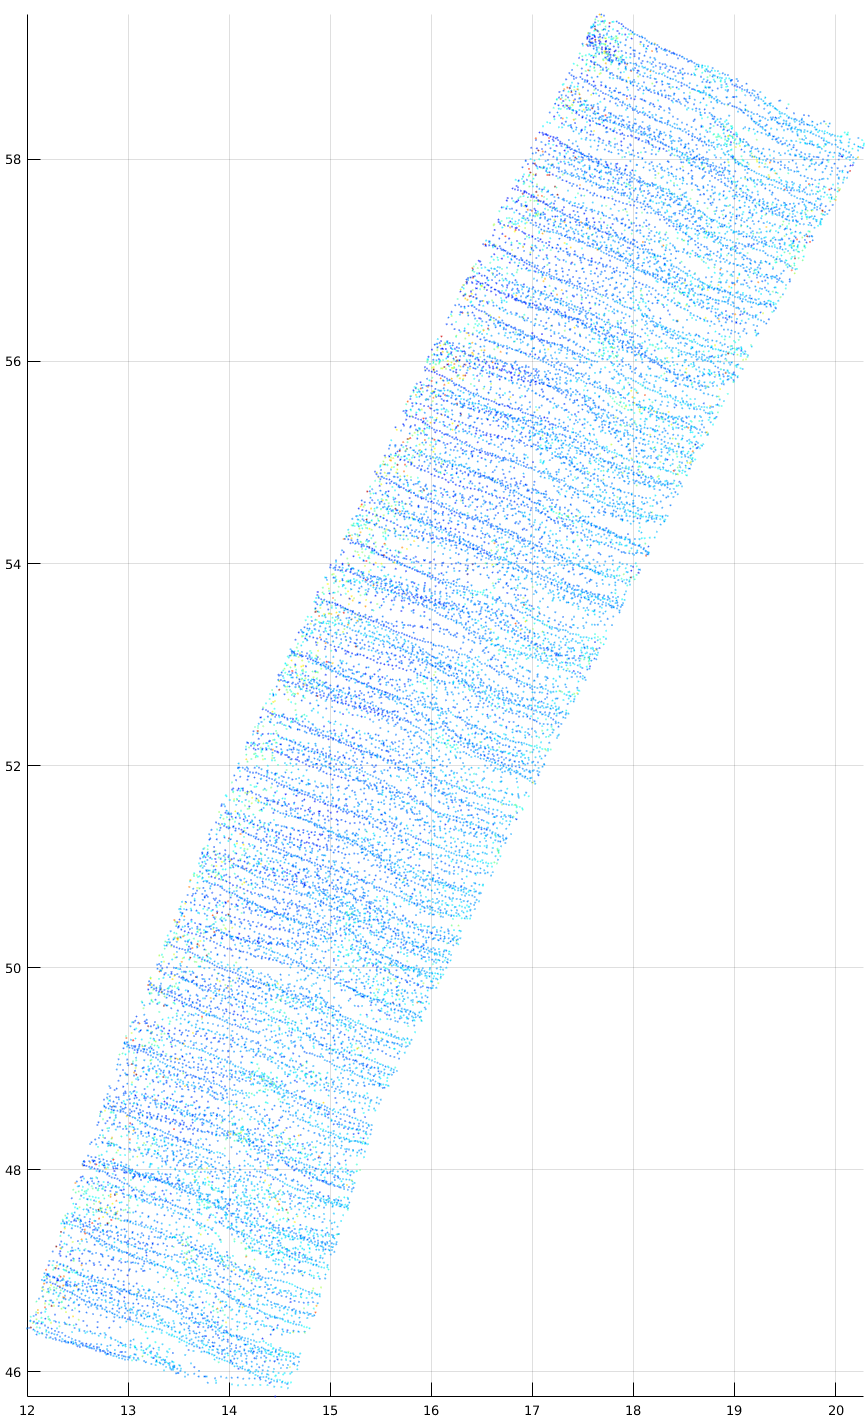
\includegraphics[width=1.0\linewidth,height=8.0 cm,keepaspectratio]{Defense_Images/visual_verification_1}
						\caption[Bean Hollow Road Satellite View]{}
						\label{fig:post_area_selected}
					\end{subfigure}
					\begin{subfigure}{0.45\textwidth}
						\centering
						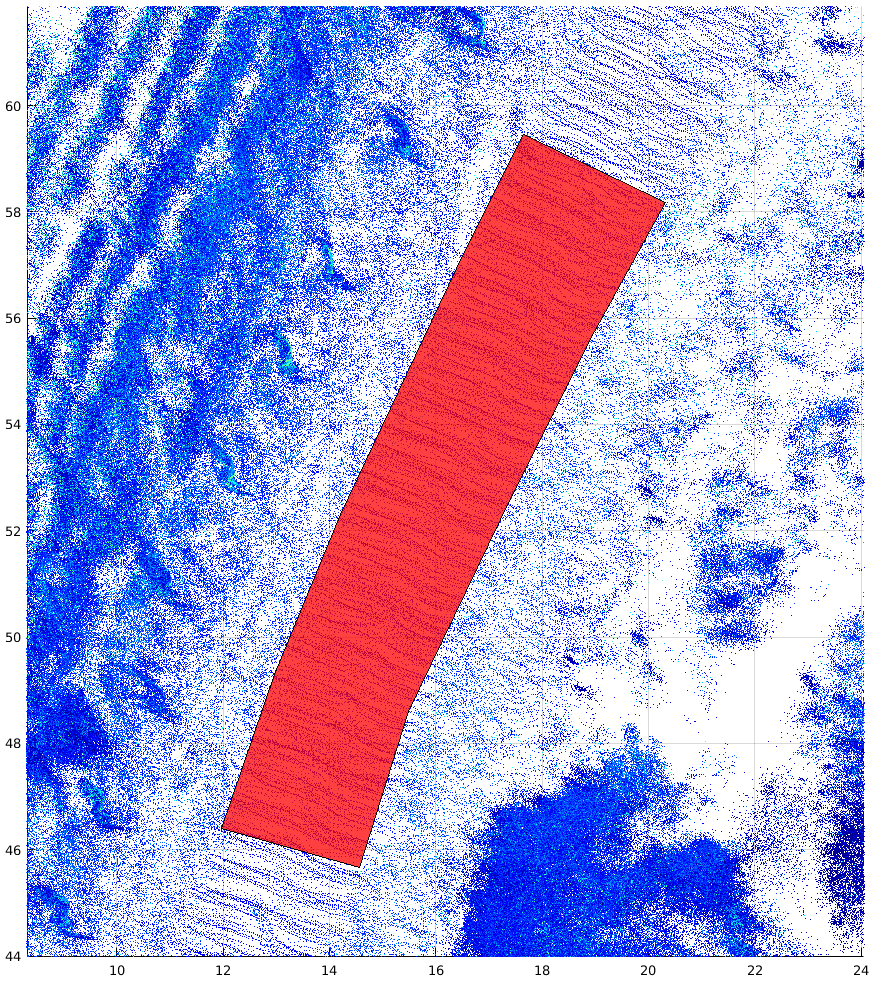
\includegraphics[width=1.0\linewidth,height=8.0 cm,keepaspectratio]{Defense_Images/post_area_selected}
						\caption[Bean Hollow Road Camera View]{}
						\label{fig:visual_verification_1}
					\end{subfigure}
					\caption[Manual Classification Visual Verification]{Scanning LiDAR point cloud data lying within a manually defined area is extracted and visually verified (a). Areas that have been verified are projected over the point cloud (b).}
					\label{fig:Visual_Verification}
				\end{figure}
	
				{}	
				
				{Manually defined and approved areas were then be saved to disk and projected unto the point cloud map. Consecutive scanning LiDAR data within the boundaries of the manually define areas was extracted. Consecutive scans requires a MATLAB transformation matrix object using GPS and IMU data \ref{sec:grab_tform}. RANSAC and Method of Least Squares was used to project a reference plane unto each consecutive LiDAR scan. For each area, each of the LiDAR 32 channels were individually examined. Because each channel represents a 360$^\circ$ sweep, the channel must be split into front and rear halves if the area being examined is gravel or chipseal, or be split into right and left halves if the area being examined is grass or foliage (Figure \ref{fig:points_front_rear}). This was done as the two halves may be substantially different and when performing feature calculations when they are not split may result in an inaccurate representation of the data. This process also closely mimics the first method of training and verification data extraction. Scanning LiDAR data was then extracted from the two halves by comparison to the manually defined areas and saved to disk.}

				\begin{figure}[H]
					\centering
					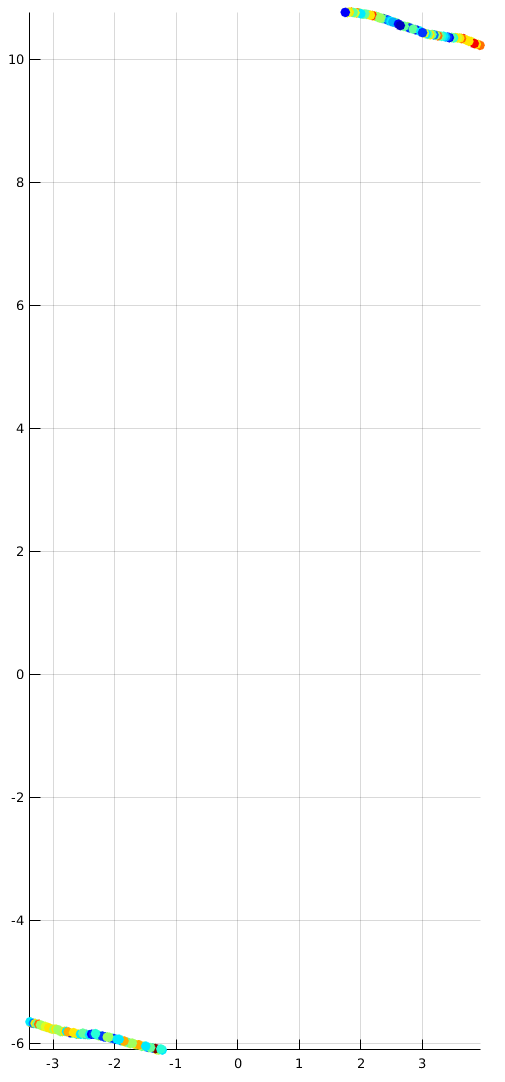
\includegraphics[width=0.5\linewidth]{Defense_Images/both_front_rear}
					\caption[Front and Rear Points]{Each scanning LiDAR channel may have points in front and behind of the vehicle that lie on a manually defined area. These must be separated, otherwise extracted features may not accurately represent consecutive points. }
					\label{fig:both_front_rear}
				\end{figure}				
				
				\begin{figure}[H]
					
					\subfloat[]{%
						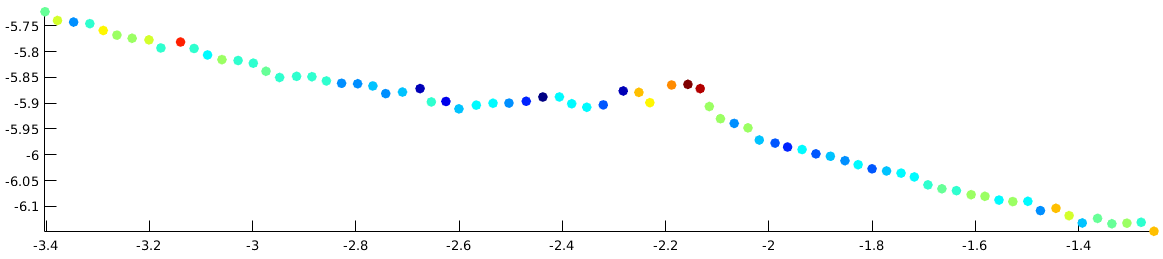
\includegraphics[clip,width=1.0\columnwidth]{Defense_Images/back_points_2}
					}
					
					\subfloat[]{%
						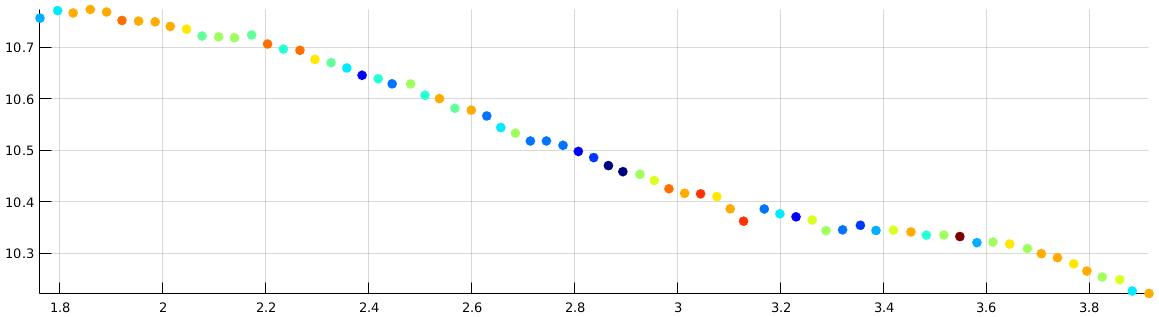
\includegraphics[width=1.0\columnwidth]{Defense_Images/front_points_2}
					}
					
					\caption[Front and Rear Point Extraction]{Rear (a) and front (b) points may be extracted}
					
					\label{fig:points_front_rear}
					
				\end{figure}	

			} % End Training and Verification Data Selection Process
		
		\newpage
			
			\subsubsection{Feature Extraction}\label{sec:Feat_Extract} {
			
				{Feature extraction was completed by performing mathematical functions on the gathered spatial and remission training data. Reference plane normal vector and distance from origin $[a,b,c,d]$ data derived from either RANSAC or Method of Least Squares methods was selected. Mean XY, Range, and mean range are calculated \ref{fig:xy_vs_range}. Per-point distance from the reference plane was calculated. Approximately 120 features were then be calculated and saved to disk.}
				
				{Features extracted include the following:}

				\begin{multicols}{2}
					\begin{itemize}[itemsep=3pt]
						\item Standard Deviation
						\item Roughness
						\item Min Max Ratio
						\item Min Squared Max Ratio
						\item Gradient
					\end{itemize}
					\vfill\null
					\begin{itemize}[itemsep=3pt]
						\item $std$
						\item $max - min$
						\item $min / max$
						\item $min^2 / max$
						\item $sqrt(sum(Gradient\*))$
					\end{itemize}
					\vfill\null
					\label{lst:feature_list}
				\end{multicols}
			
				{where $Gradient$ refers to the difference between consecutive numbers in an array.}
			
			\newpage
				
			} % End Feature Extration
		
			\subsection{Feature Data Sets}\label{sec:feature_data_sets} {
								
				{Six feature sets were considered when creating the Random Decision Forest algorithms, resulting in six total classifiers. Note that range from origin to a point was calculated using the X, Y, and Z coordinates and Pythagorean's Theorem, as range was not directly given in the LiDAR rosbag messages. This lengthens the amount of time required for feature extraction. Future work may include altering the incoming data stream to give range directly in order to increase computational efficiency. To consider distance from the LiDAR origin, features were divided by the average distance from the origin.}
				
				\begin{itemize}[itemsep=1pt]
					\item All 
					\begin{itemize}[itemsep=1pt]
						\item Features extracted using height from projected reference plane, height from the LiDAR origin, and range from the LiDAR origin
						\item 60 features in total
						\item Two RDFs were created using RANSAC and MLS as plane projection methods
						\item Distance from origin considered by creating two additional feature data sets per reference point by dividing each feature set (\ref{lst:feature_list}) by average range or X, Y distance. 
					\end{itemize}
					\item Top Twenty 
					\begin{itemize}[itemsep=1pt]
						\item Features extracted using height from projected reference plane, height from the LiDAR origin, and range from the LiDAR origin
						\item Top twenty features from all features, determined by number of instances
						\item Two RDFs were created using RANSAC and MLS as plane projection methods
						\item Distance from origin considered by creating two additional feature data sets per reference point by dividing each feature set (\ref{lst:feature_list}) by average range or X, Y distance.
					\end{itemize}
					\item ZXY
					\begin{itemize}[itemsep=1pt]
						\item 20 features total
						\item Features extracted using the height from LiDAR origin only
						\item Distance from origin considered by creating an additional feature data set by dividing with the average X, Y distance
					\end{itemize}
					\item Range
					\begin{itemize}[itemsep=1pt]
						\item 20 features total
						\item Features extracted using the range from LiDAR origin only
						\item Distance from origin considered by creating an additional feature data set by dividing with the average range
					\end{itemize}
				\end{itemize}
		
			} % End Feature Data Set
			
			\subsubsection{Random Decision Forest Creation}\label{sec:random-decision-forest-creation}{
			
				{MATLAB's $TreeBagger$ function was used to create Random Decision Forests (see \ref{RDF_SECT} for a detailed overview of the function and input arguments). Included features, number of binary splits, and number of trees were principal guiding factors in RDF creation. Features to be included in the training data set was determined by examination of feature usage in each RDF and the effect on the validation accuracy. Number of bagged features followed convention of the square root of total number of features. Individual tree depth was determined by examination of the validation accuracy. Larger number of splits may lead to more accurate results at the expense of computational efficiency. } 

				
%				\begin{figure}[H]
%					\centering
%					\includegraphics[width=0.5\linewidth]{Defense_Images/}
%					\caption[]{}
%					\label{fig:}
%				\end{figure}
%				

				
			} % End Random Decision Forest Creation

	
			\subsubsection{Random Decision Forest Verification}\label{sec:random-decision-forest-verification}{
			
				{Random Decision Forest classification accuracy was verified by passing the algorithm a verification data set. Verification data was similar to that of the training data, however was not part of the training data. Random Decision Forests of increasing sizes were tested individually using MATLAB's $predict$ function. Accuracy, true positive for road surface prediction, and false negative prediction for road surface detection scores were then calculated and plotted (Figure \ref{fig:Example_Err_Plts}).}

				\begin{figure}[H]
					
					\subfloat[]{%
						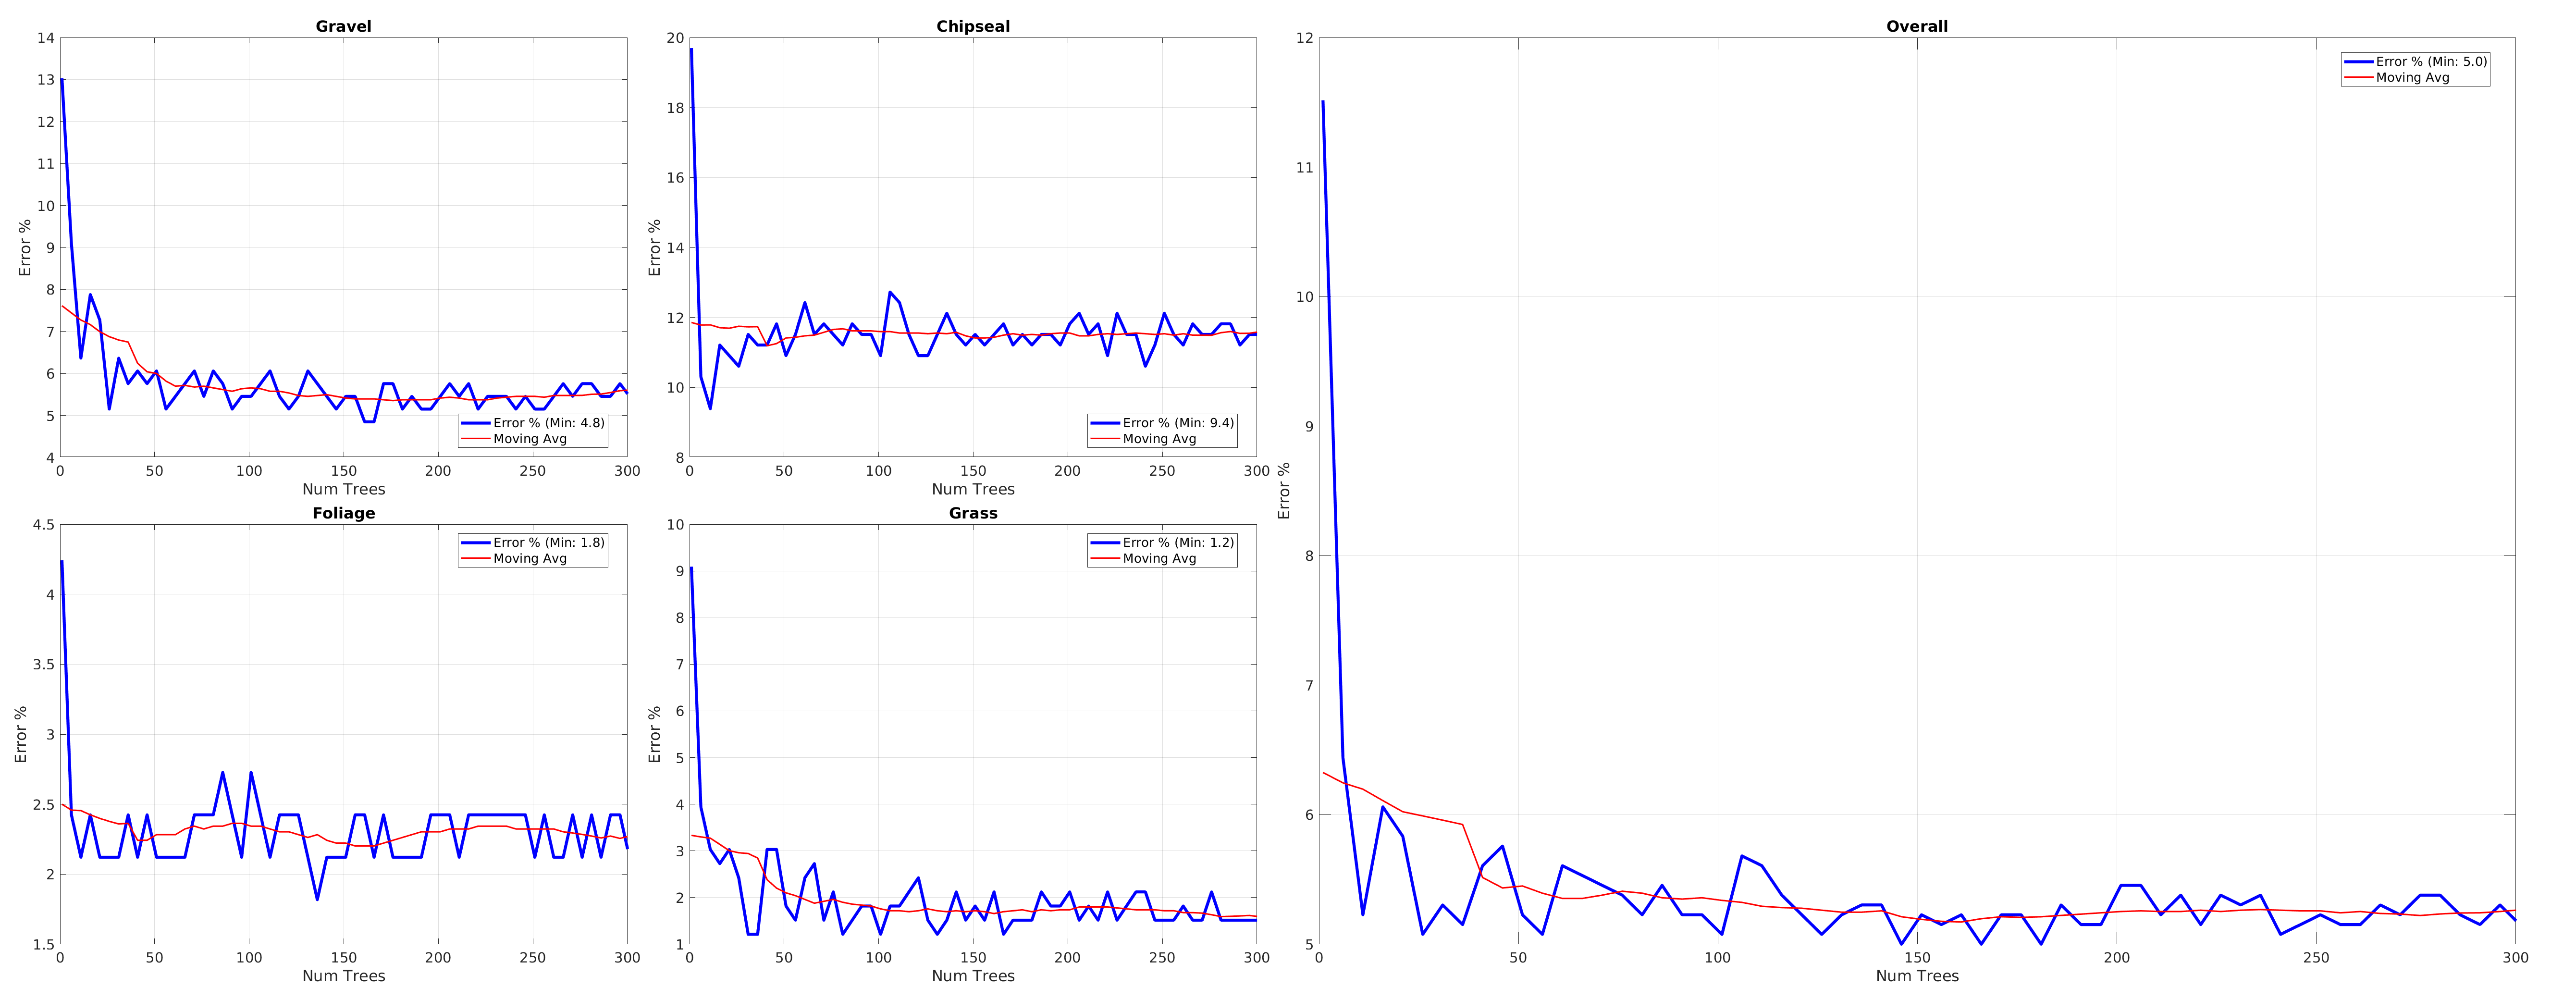
\includegraphics[clip,width=1.0\columnwidth]{Defense_Images/MLS_ALL_200D_err_sub_plot}
					}
					
					\subfloat[]{%
						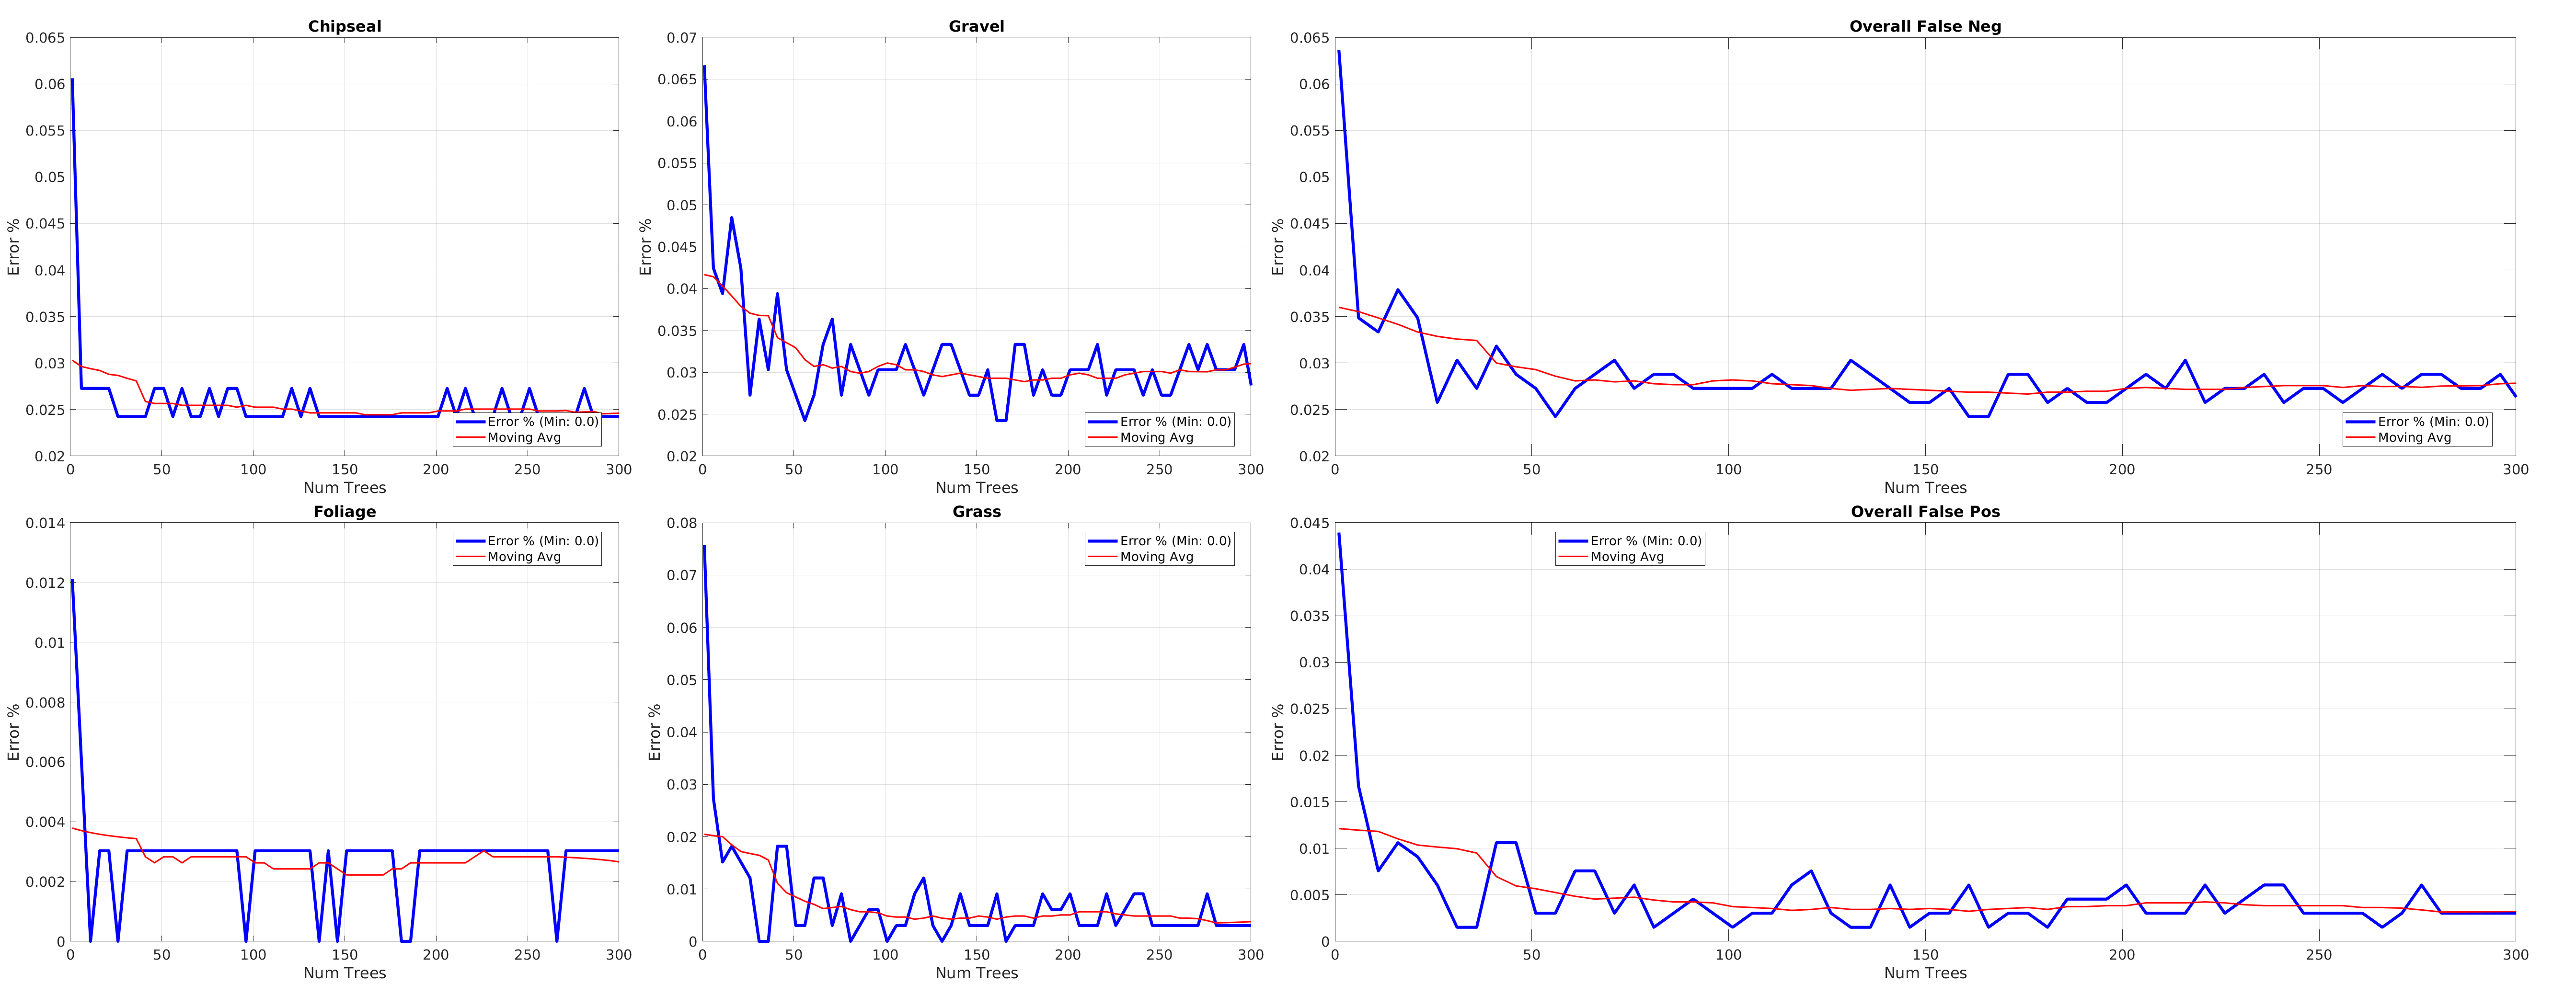
\includegraphics[width=1.0\columnwidth]{Defense_Images/MLS_ALL_200D_false_pos_neg_sub_plot}
					}
					
					\caption[Validation Error Example Plots]{Overall and individual class prediction accuracy was completed (a). Overall and individual true positive and false negative identification of a road surface (gravel/chipseal) was completed (b).}
					
					\label{fig:Example_Err_Plts}
					
				\end{figure}
	
			} % End Random Decision Forest Verification
						
							
			\subsubsection{Random Decision Forest Optimization}\label{sec:random-decision-forest-optimization}{
				
				{Optimization of Random Decision Forests was achieved by testing accuracy and rate of classification between RDFs with varying number of features and trees. Optimization feature usage was achieved by counting feature usage in each RDF. Histograms were created by loading a directory with a series of RDFs. Each tree was examined for feature usage. Feature usage was counted and displayed in a histogram plot (Figure \ref{fig:feat_use_top_ten_example}). }		

				\begin{figure}[H]
					\centering
					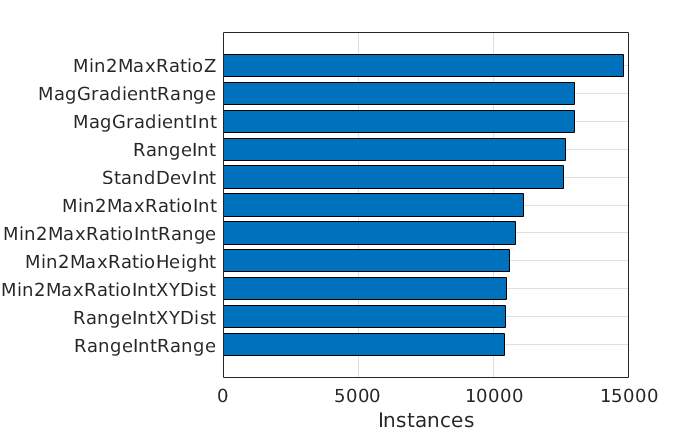
\includegraphics[width=0.7\linewidth]{Defense_Images/feat_use_top_ten_example}
					\caption[Example Feature Use Histogram]{Feature use may be visually examined by considering the usage per tree in the RDF. Here shown is the top ten features used from a series of RDFs. }
					\label{fig:feat_use_top_ten_example}
				\end{figure}
			
				{RDF accuracy was validated using the process in the previous section (\ref{sec:random-decision-forest-verification}). Successfully trained RDFs will have an increase in accuracy as the number of trees grow, however there is a point of diminishing returns. Furthermore, the RDF may become over-trained if grown too large (\ref{RDF_SECT}), and larger RDFs are computationally expensive to use. Therefore, accuracy verses number of trees was examined to determine the optimal RDF size. There is no convention on methodology, and is generally approached on a case by case instance in literature. For this work, number of trees in the RDF was determined by examination of the out-of-bag error where the change in moving average of the validation error falls below 0.275\% and is within 15\% of the minimum error (Figure \ref{fig:Overall_Error_Early_Stopping}).}
				
				\begin{figure}[H]
					\centering
					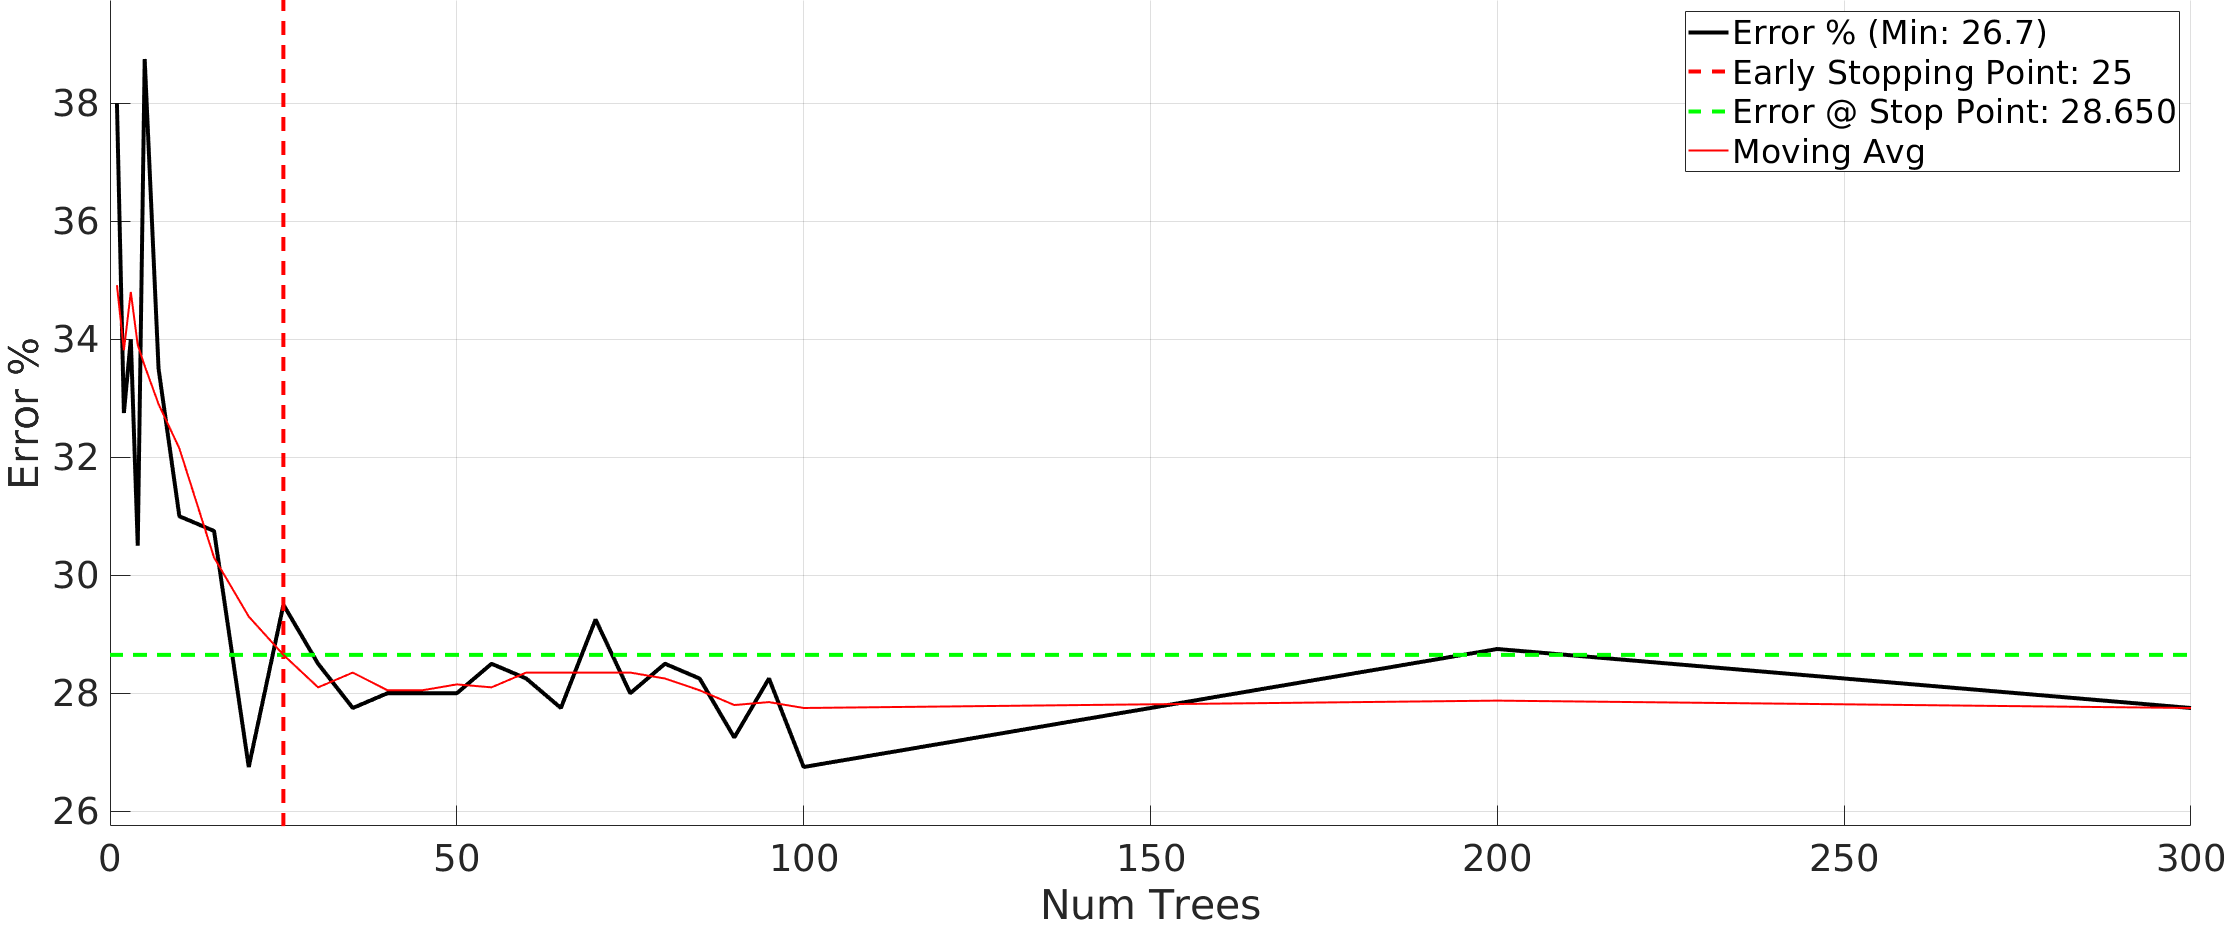
\includegraphics[width=0.75\linewidth]{Defense_Images/Overall_Error_Early_Stopping}
					\caption[Validation Error versus RDF Size]{Validation error was calculated and a potential early stopping point was found when the \% change in error falls below 0.275\%.}
					\label{fig:Overall_Error_Early_Stopping}
				\end{figure}
				
				{Scanning LiDAR data was discretized into quadrants (Figure \ref{fig:channel_split_multi}). Quadrant size affects terrain classification accuracy at the expense of granularity of results and computational time. Smaller quadrants allow for greater resolution of terrain classification, however more computational time is required. Larger quadrants allow for swifter classification, however as consecutive scanning LiDAR points may include road and non-road surfaces, classification accuracy and road edge detection capability may suffer.}
				
				\begin{figure}[H]
					\centering
					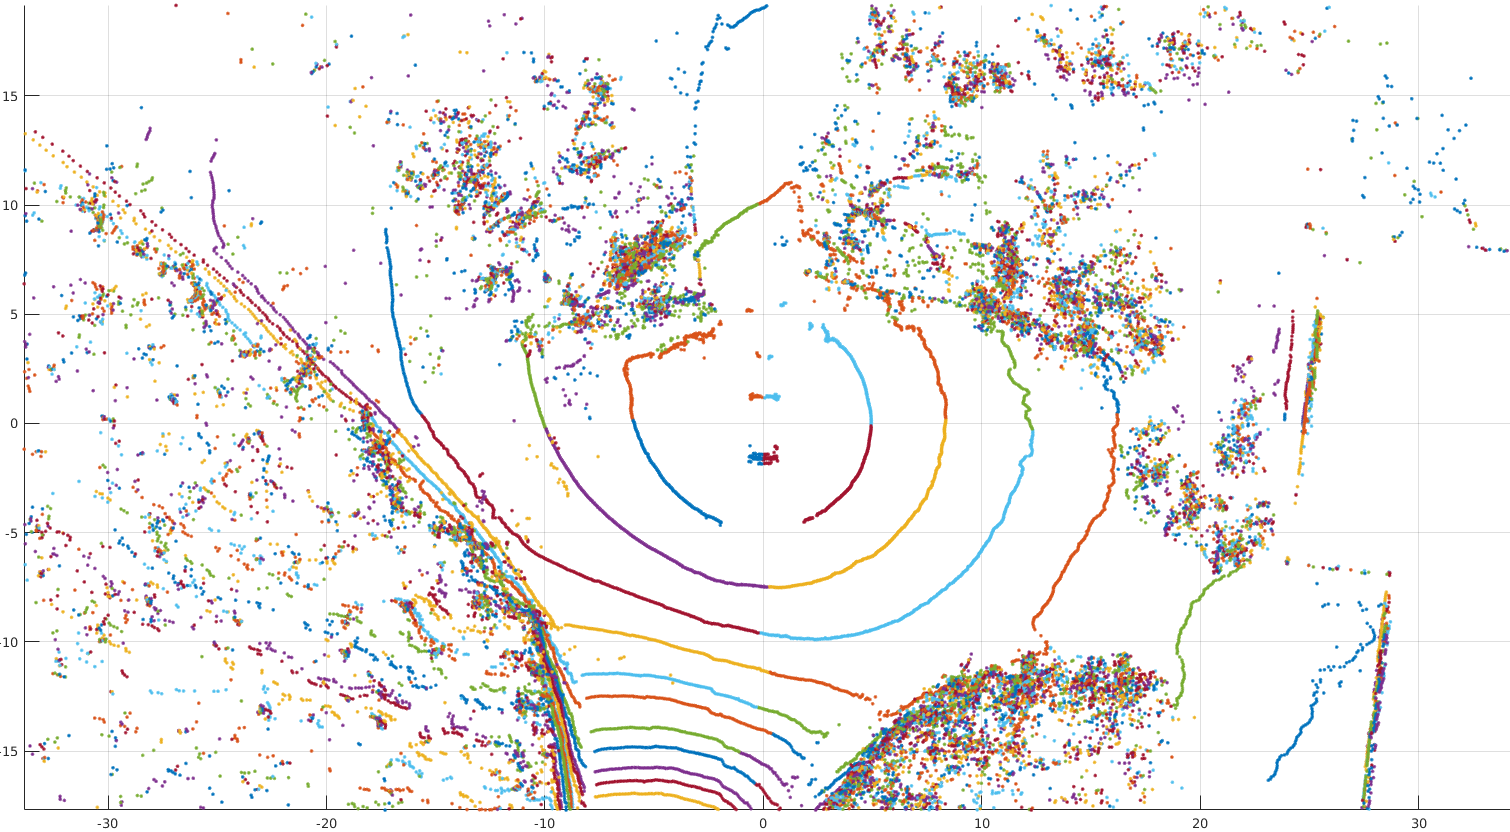
\includegraphics[width=0.7\linewidth]{Defense_Images/channel_split_multi}
					\caption[Quadrants Discretization]{Point cloud data was discretized, in this case into quadrants. }
					\label{fig:channel_split_multi}
				\end{figure}
				
			} % End Random Decision Forest Optimization
				
				
			\subsubsection{Random Decision Forest Testing}{
			
				{Basic functionality of scanning LiDAR point cloud classification using Random Decision Forests was completed by considering individual point clouds. While results were not scored for accuracy, as this would be completed later using combined point cloud data (), this process gave a rough visual estimation of accuracy. Results were visually compared to satellite imagery by manually fitting the point cloud to the origin's gps coordinates and rotating the point cloud until it matched the satellite imagery (Figure \ref{fig:all_feat_overlay}). }
				
				\begin{figure}[H]
					\centering
					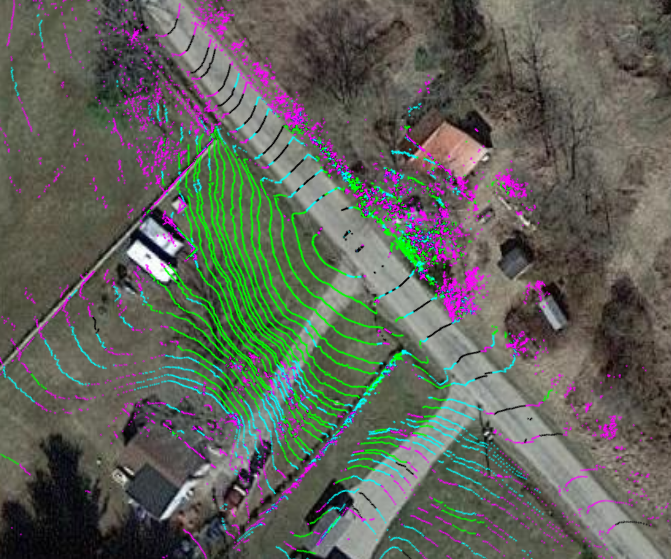
\includegraphics[width=0.7\linewidth]{Defense_Images/all_feat_overlay}
					\caption[Classified Single Point Cloud]{Point cloud data was overlayed unto satellite imagery to visually confirm RDF performance.}
					\label{fig:all_feat_overlay}
				\end{figure}

				
				
			} % End Random Decision Forest Testing
				
		} % End Obj 1 Task 2

	} %End Objective 1


\newpage
	
	\section{Objective 2}\label{sec:objective-2}
	
		{
		
		\textbf{Objective Statement: Automate detection of consecutive LiDAR scans of unmarked chipseal and gravel roads and verify using manually defined road boundaries.}
		
		\subsection{Task 1}{
		
			\textbf{Task 1: }{Determine method of synchronizing LiDAR, GPS, and IMU data in order to determine point cloud position and orientation}
		
				{Compiling smaller point clouds into a larger point cloud requires the determination of origin and orientation of each point cloud. Employing GPS and IMU data to determine position and orientation respectively, while not as robust as more advance methods such as Iterative Closest Point, was sufficient for analysis of smaller stretches of road. Physical distance between the GPS, IMU, and LiDAR were rectified by measuring the distance between the modules. Reference frames between the GPS, IMU, and LiDAR was completed by applying rotational matrices. Transformation matrices were created by considering the GPS position and the IMU's roll, pitch, and yaw data. Point cloud data was then altered with the resulting transformation matrices, and consecutively stored to an overall point cloud array.}
			
			\subsubsection{Transformation Matrix Derivation} \label{sec:grab_tform} {
			
				{Point cloud translation and rotation was accomplished using transformation matrices that were derived from GPS and IMU data stored in a rosbag. GPS and IMU  time stamps that most closely matched LiDAR timestamps were found. Rotation matrices were created using extracted roll, pitch, and yaw data from the IMU. LiDAR origin was found using GPS longitude, latitude, and altitude data. Physical distances between the GPS, IMU, and LiDAR was rectitude by obtaining reference frames provided by AutonomouStuff (\ref{sec:experimental-apparatus-setup}). GPS coordinates were offset by the current orientation and converts the ground truth to the LiDAR frame. GPS, IMU, and LiDAR reference frames and rotational updates were combined into trajectory vectors. Transformation matrices were then derived using MATLAB's $rigid3d$ function. Consecutive point cloud scans may then translated and rotated with derived transformation matrices (Figure \ref{fig:Compiled_PCD}).}
				
				\begin{figure}[H]
					\centering
					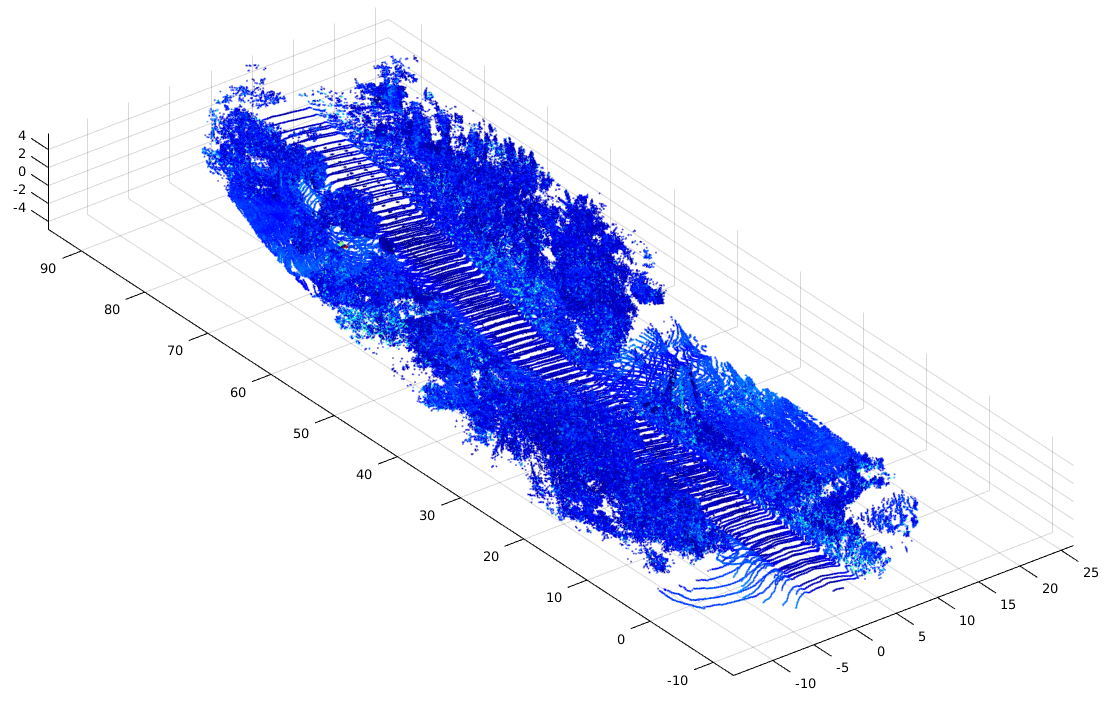
\includegraphics[width=0.7\linewidth]{Defense_Images/Compiled_PCD}
					\caption[Compiled Point Cloud Data]{Compiled Point Cloud Data}
					\label{fig:Compiled_PCD}
				\end{figure}
				
			} % End Transformation Matrix Derivation

		
		} % End Obj 2 Task 1
		
		\subsection{Task 2}\label{sec:Objective_2_Task_2}{
		
			{\textbf{Automate detection of consecutive LiDAR scans of unmarked chipseal and gravel roads and verify using manually defined road boundaries.} LiDAR, GPS, and IMU data of physical unmarked gravel and chipseal roads was collected. Road surface area was predicted using the model developed in Objective 1. GPS and IMU data allowed for the creation of transformation matrices required for stitching consecutive LiDAR scans. Stitched results were then scored by comparing them to manually defined road surfaces. Completion of Objective II was accomplished by achieving the goal of classifying consecutive LiDAR scans of unmarked chipseal and gravel roads. Success of Objective II was measured by determining the accuracy of detection and processing time. The outcome of Objective II is a method of detecting a stretch of an unmarked gravel or chipseal road with a scanning LiDAR sensor.}
			
			\subsubsection{Consecutive Point Cloud Classification}\label{sec:consecutive_point_cloud_classification}{
			
				{Consecutive scanning LiDAR scans were saved to disk as point clouds with the process described in \ref{sec:data_processing}. Each point cloud was classified using the derived Random Decision Forest algorithm in Objective 1. Scanning LiDAR data to be classified was limited to channels two through four counting upwards from the channel with the highest deflection angle below horizontal in order to decrease computational time. Classification results were waved to disk. GPS and IMU data with closest matching timestamps to the consecutive LiDAR scans were used to create the transformation matrix derivation in the process described in \ref{sec:grab_tform} and were subsequently saved to disk. Consecutive classification results were loaded from disk then transformed and rotated with its corresponding transformation matrix. Combined classified point clouds were saved to disk.}
				
			}
			
			\subsubsection{Consecutive Point Cloud Classification Scoring}\label{sec:consecutive_point_cloud_classification_scoring}{
			
				{Scoring combined consecutive classification results was accomplished by comparing to manually defined areas. Manually defined areas were derived using the process described in \ref{sec:training_and_verification_data_selection_process}. Classification results that were sympatric to manually defined areas were extracted and examined for accuracy. Road detection accuracy was determined by scoring the exact terrain classification, true positive road surface detection, and false negative road surface detection. Side-of-road areas were considered for road edge detection. Drop off in positive road surface classification rates of 50\% or greater in side-of-road areas would be indicative that the random decision forest classification algorithm was adequate at detecting the road edge.}
				
			}
		
		} % End Obj 2 Task 2

	} % End Objective 2
	
} % End Methodolgy


\newpage
	
	
	\section{Summary of Methods}\label{sec:summary-of-methods}
	{
		
		{Point cloud data was used to take advantage of an unmarked road's surface noise profile by projecting a reference plane and examination of point height variance. Objective I explored physical point cloud data for identifying a model for describing a gravel road such that a vehicle may be able to predict road surface area based on terrain classification. The outcome of Objective I was a terrain classification approach to describing gravel road surface point cloud data. Objective II explored using the model derived in Objective I to automatically detect a stretch of an unmarked road surface. The outcome of Objective II was automated detection of consecutive LiDAR scans of unmarked gravel and chipseal roads.}
		 
		{\textbf{Final Deliverable:} Method for physical gravel and chipseal road detection by using a terrain classification approach to predicting road surface area.}
		
	} % End Summary of Methods

\chapter{Results}{
	
	\section{Training Data Collection}\label{sec:training-data-collection}{
	
		{Scanning LiDAR, GPS, and IMU data was collected on closed lots and public roads near Athens Ohio using the Experimental Apparatus. Point cloud data from the resulting rosbags was manually defined by area as one of four basic terrain types: gravel, chipseal, foliage, or grass. Gravel data was gathered from the closed gravel lot maintained by the Ohio University Civil Engineering Department (Figure \ref{fig:gravel_lot_example}). Chipseal data was gathered from unmarked public roads (Figure \ref{fig:chipseal_road_example}). Grass data, defined as well-trimmed lawn grass, and foliage, defined as leafy trees and bushes, was gathered from areas surrounding public roads. }
		
		\begin{figure}[H]
			\centering
			\includegraphics[width=0.7\linewidth]{Defense_Images/gravel_lot_example}
			\caption[Example of Gravel Road]{Gravel lot maintained by the Ohio University Civil Engineering Department}
			\label{fig:gravel_lot_example}
		\end{figure}
		
		\begin{figure}[H]
			\centering
			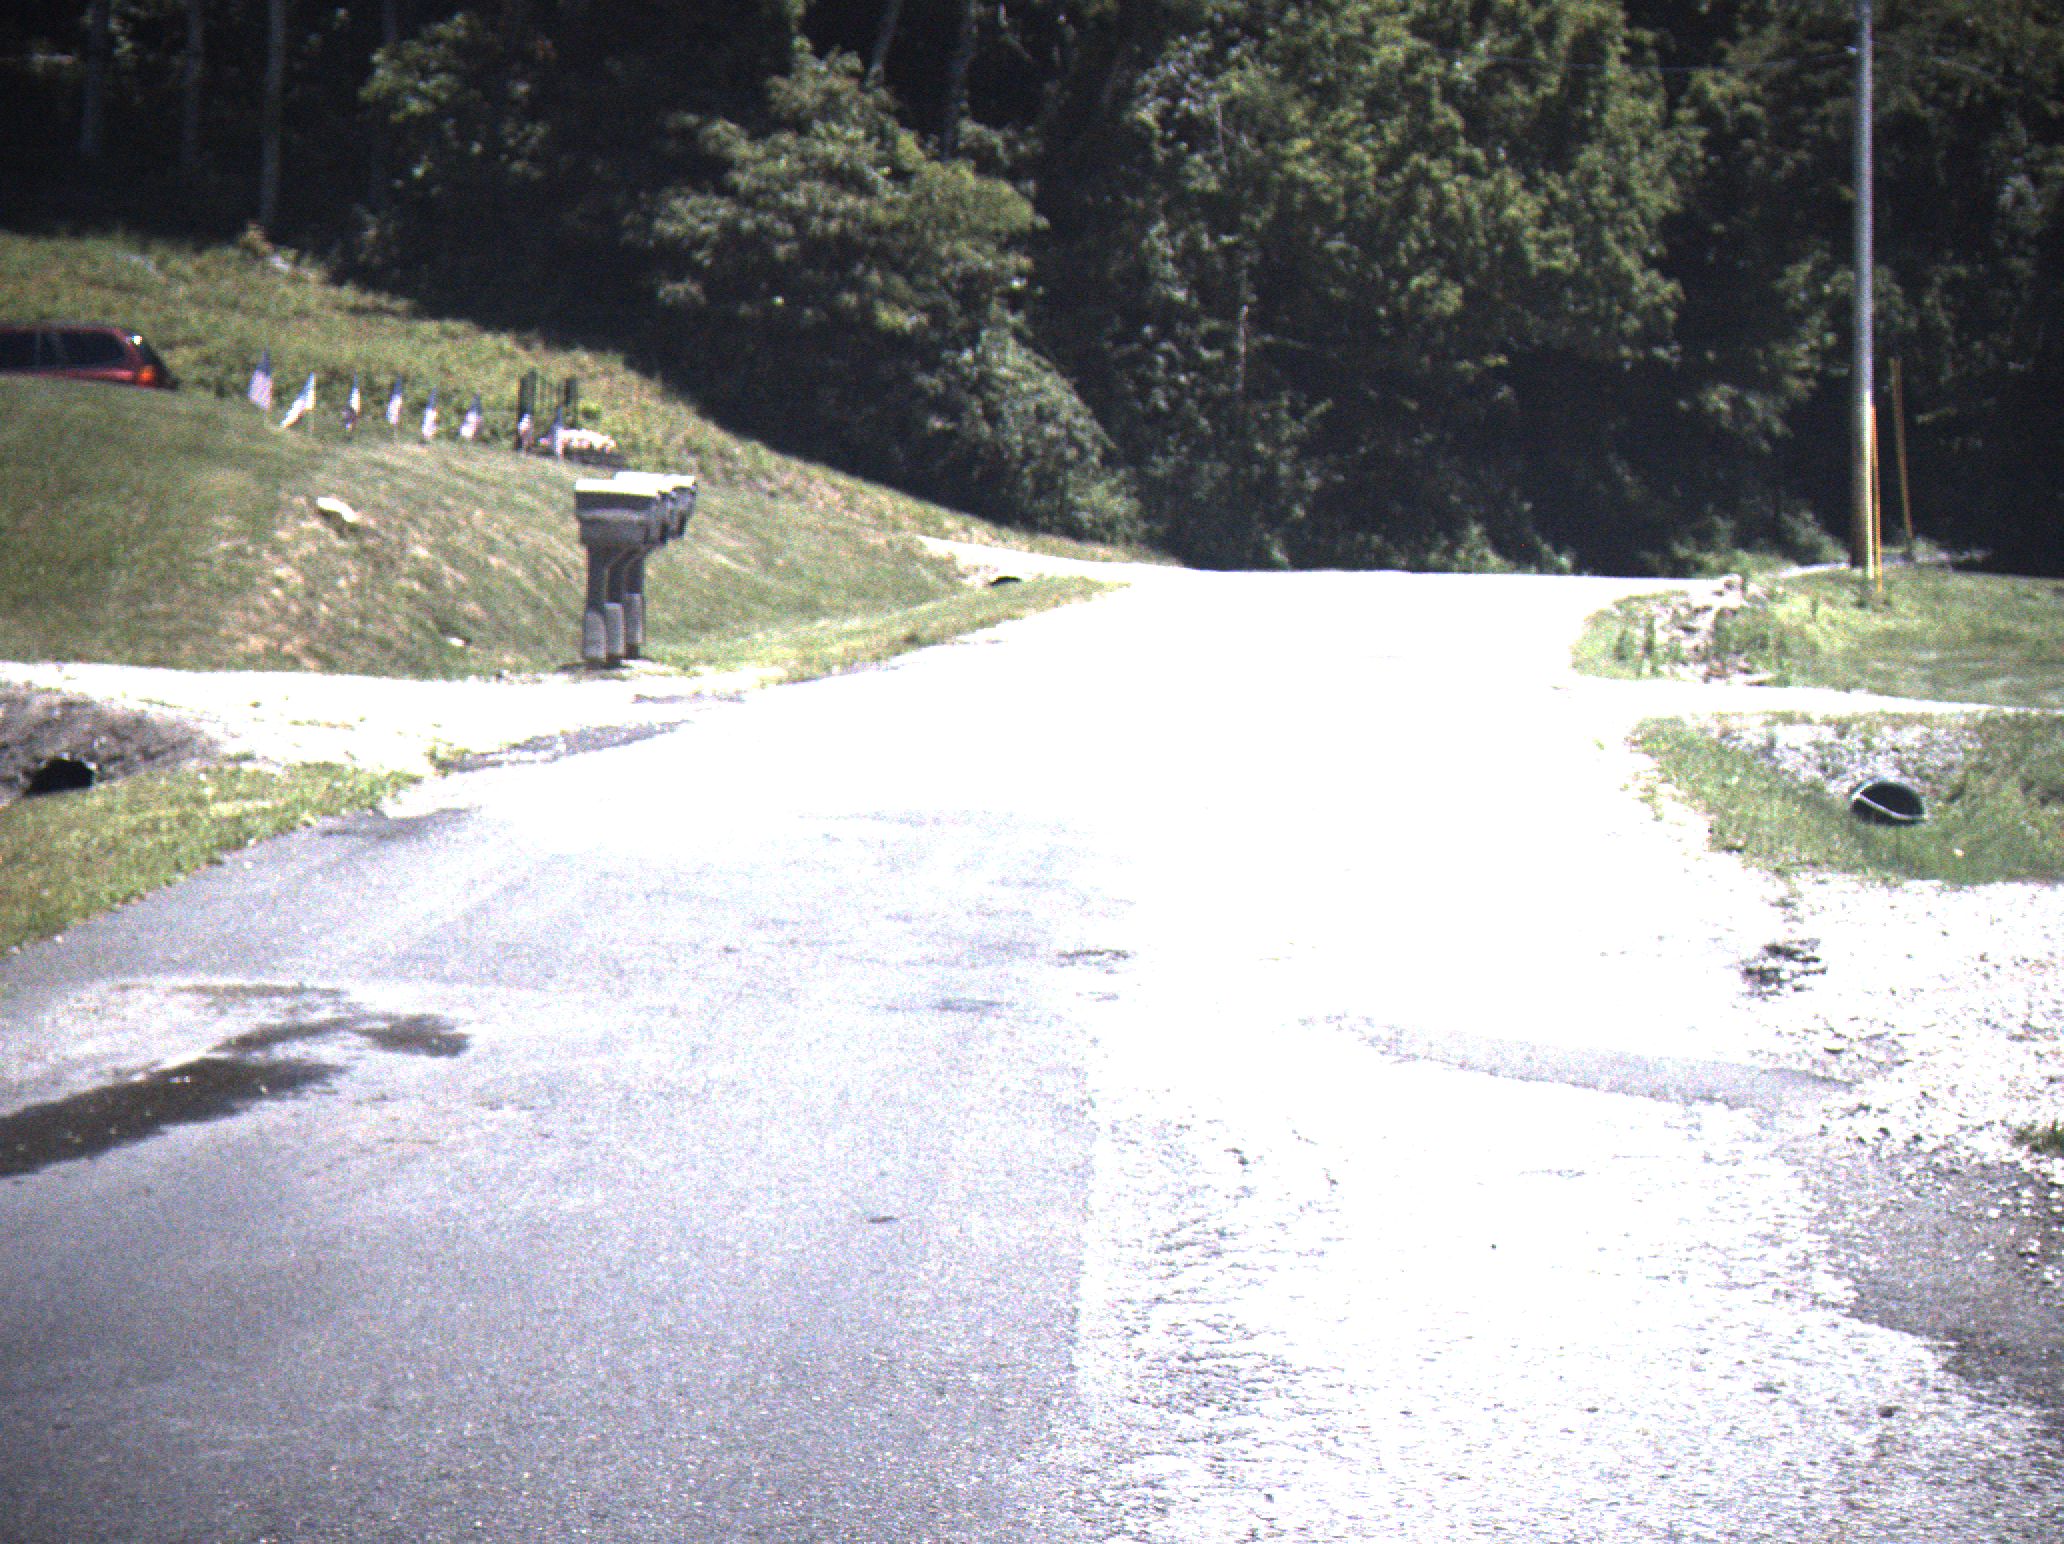
\includegraphics[width=0.7\linewidth]{Defense_Images/chipseal_road_example}
			\caption[Example of Chipseal Road]{Example of a chipseal road with intercepting gravel driveways}
			\label{fig:chipseal_road_example}
		\end{figure}
	
	}
	
	\section{RANSAC vs Method of Least Squares}\label{sec:ransac-vs-method-of-least-squares}{
	
		{Point cloud data often includes hills, buildings, trees, and other vertical features that may pose a challenge in obtaining close a fitting projected plane to a road surface. Some features, such as minimum, maximum, or average distance to the projected plane, cannot be used as terrain classification performance would suffer should plane fitment be poor. Method of Least Squares proved to be the least computationally expensive, with an average time of 1.401 ms versus 4.888 ms for RANSAC (Figure \ref{fig:RANSAC_vs_MLL}). }
		
		\begin{figure}[H]
			\centering
			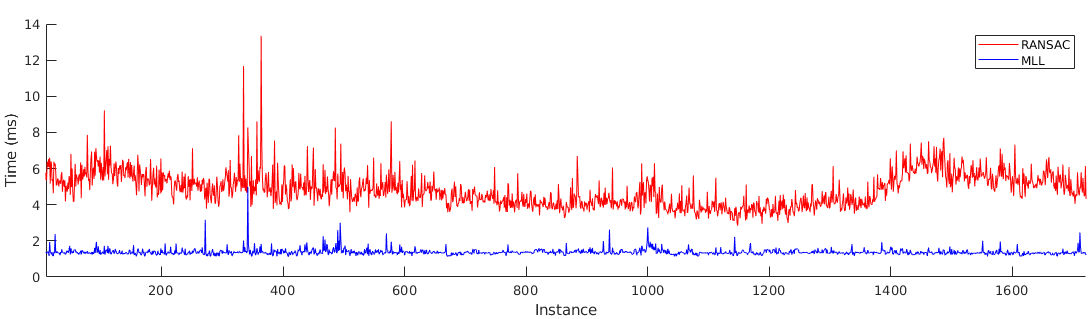
\includegraphics[width=1.0\linewidth]{Defense_Images/RANSAC_vs_MLL}
			\caption[RANSAC vs MLS Compute Times]{Time of computation for plane projection comparison between RANSAC (red) and Method of Least Squares (blue). }
			\label{fig:RANSAC_vs_MLL}
		\end{figure}
	
		{MATLAB's  $pcplanefit$ function \cite{MATLAB_PCFITPLANE} was used for RANSAC plane projection. Passed arguments to effect the processing time and results include threshold distance and maximum number of iterations. Threshold distance was found to significantly effect the computational load (Figure \ref{fig:RANSAC_threshold}), with a 93.0937\% difference between the maximum and minimum values tested (Table \ref{tab:RANSAC_Varations}). Threshold distance for this work was defined at 1 meter, 69.9976\% different from the maximum threshold value, as close plane fitment to the road surface was later determined to not be a major factor in terrain classification, as hills and other natural topographical features may limit plane fitment scores. Future research may include further increasing the threshold size to decrease computational load. Maximum number of iterations was left at the default 1000 iterations, as lowering the number of iterations has negligible effect on computational time (Figure \ref{fig:RANSAC_Iteration}, Table \ref{tab:RANSAC_Varations}), yielding only a 19.8622\% between the minimum and maximum tested values. Future work may include determining a method to lower iteration count while also improving computational efficiency. Projected plane model outputs is the normal vector $[a,b,c]$ and the height above the origin $d$..}
		
		\begin{figure}[H]
			\centering
			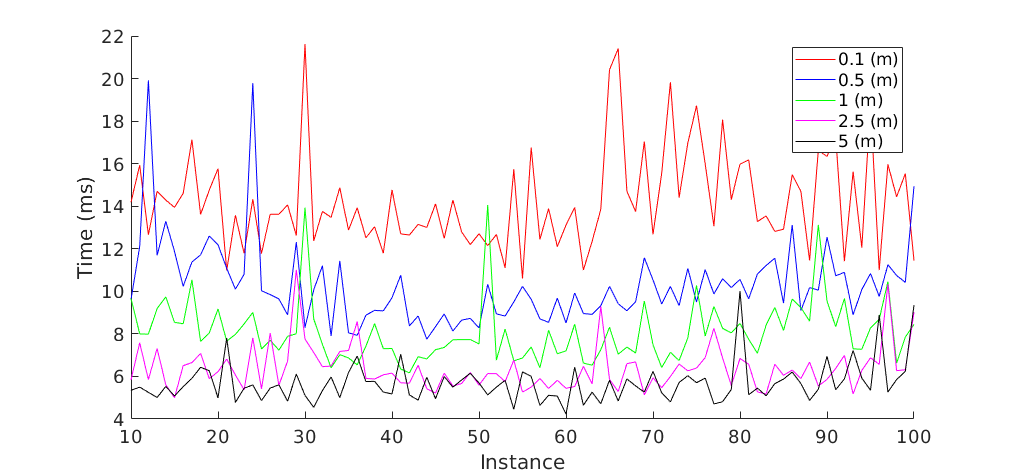
\includegraphics[width=0.7\linewidth]{Defense_Images/RANSAC_threshold.png}
			\caption[RANSAC Computation Time vs Threshold Distance]{RANSAC Computation Time vs Iteration Count. Iterations was constant at 100 iterations. Differences in computational time may be clearly observed. }
			\label{fig:RANSAC_threshold}
		\end{figure}
		
		\begin{figure}[H]
			\centering
			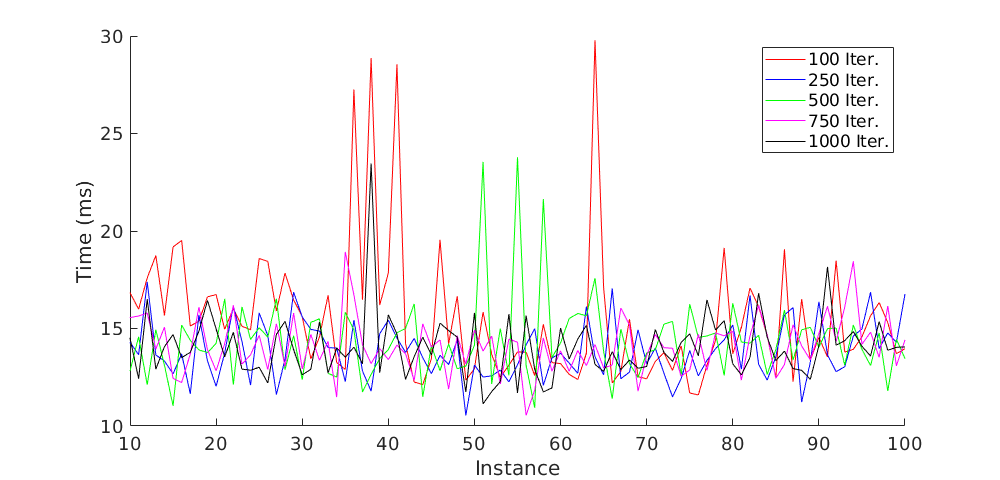
\includegraphics[width=0.7\linewidth]{Defense_Images/RANSAC_Iteration.png}
			\caption[RANSAC Computation Time vs Iteration Count]{RANSAC Computation Time vs Iteration Count. Threshold was constant at 1m. Differences in computational time is not apparent. }
			\label{fig:RANSAC_Iteration}
		\end{figure}
		

		\begin{table}[H]
			\centering
			\begin{tabular}{| >{\centering}p{2.5cm} | >{\centering}p{2.5cm} | >{\centering}p{2.5cm} | >{\centering}p{2.5cm} |} 
				\hline
				\textbf{Distance (m)} & \textbf{Time (ms)} & \textbf{Iterations} & \textbf{Time (ms)}  \tabularnewline 
				\hline
				0.1                   & 15.584             & 100                 & 0.0171              \tabularnewline 
				\hline
				0.5                   & 10.4677            & 250                 & 0.0140              \tabularnewline 
				\hline
				1.0                   & 8.1404             & 500                 & 0.0144              \tabularnewline 
				\hline
				2.5                   & 6.4184             & 750                 & 0.0141              \tabularnewline 
				\hline
				5.0                   & 5.6843             & 1000                & 0.0141              \tabularnewline
				\hline
			\end{tabular}
			\caption[RANSAC Parameter Variations]{MATLAB $pcfitplane$ parameters may be used to increase computational efficiency at the expense of fitment score. For this work two variables were considered: threshold distance and number of iterations. }
			\label{tab:RANSAC_Varations}
		\end{table}
		
	} % End RANSAC vs Method of Least Squares
		
	
	\section{Random Decision Forest Training and Verification}
	
		{MATLAB was used to load training data in order to train Random Decision Forests using the TreeBagger function. Training data for all four terrain types was loaded and features were calculated. Height and intensity features included were Standard Deviation, Roughness, Min Max Ratio, Min Squared Max Ratio, and Gradient, all of which are common features that may be extracted from point cloud data \cite{breiman_random_2001}. Multiple variations of the features were considered based on possible reference point and distance from the point of interest (Figure \ref{fig:xy_vs_range}). Three references for spatial feature extraction were considered: Perpendicular distance to the reference plane, perpendicular distance to the LiDAR origin, and the range from the LiDAR origin to the point of interest (Figure \ref{fig:xy_vs_range}). Relative distance from the LiDAR Origin was also considered, as LiDAR noise may be proportional to distance, therefore additional features were extracted by dividing the previously mentioned features by the XY Distance and Range (Figure \ref{fig:xy_vs_range}). Multiple RDFs were created using different feature sets and number of trees, which were then tested for accuracy against a verification data set.} 
	
		\begin{figure}[H]
			\centering
			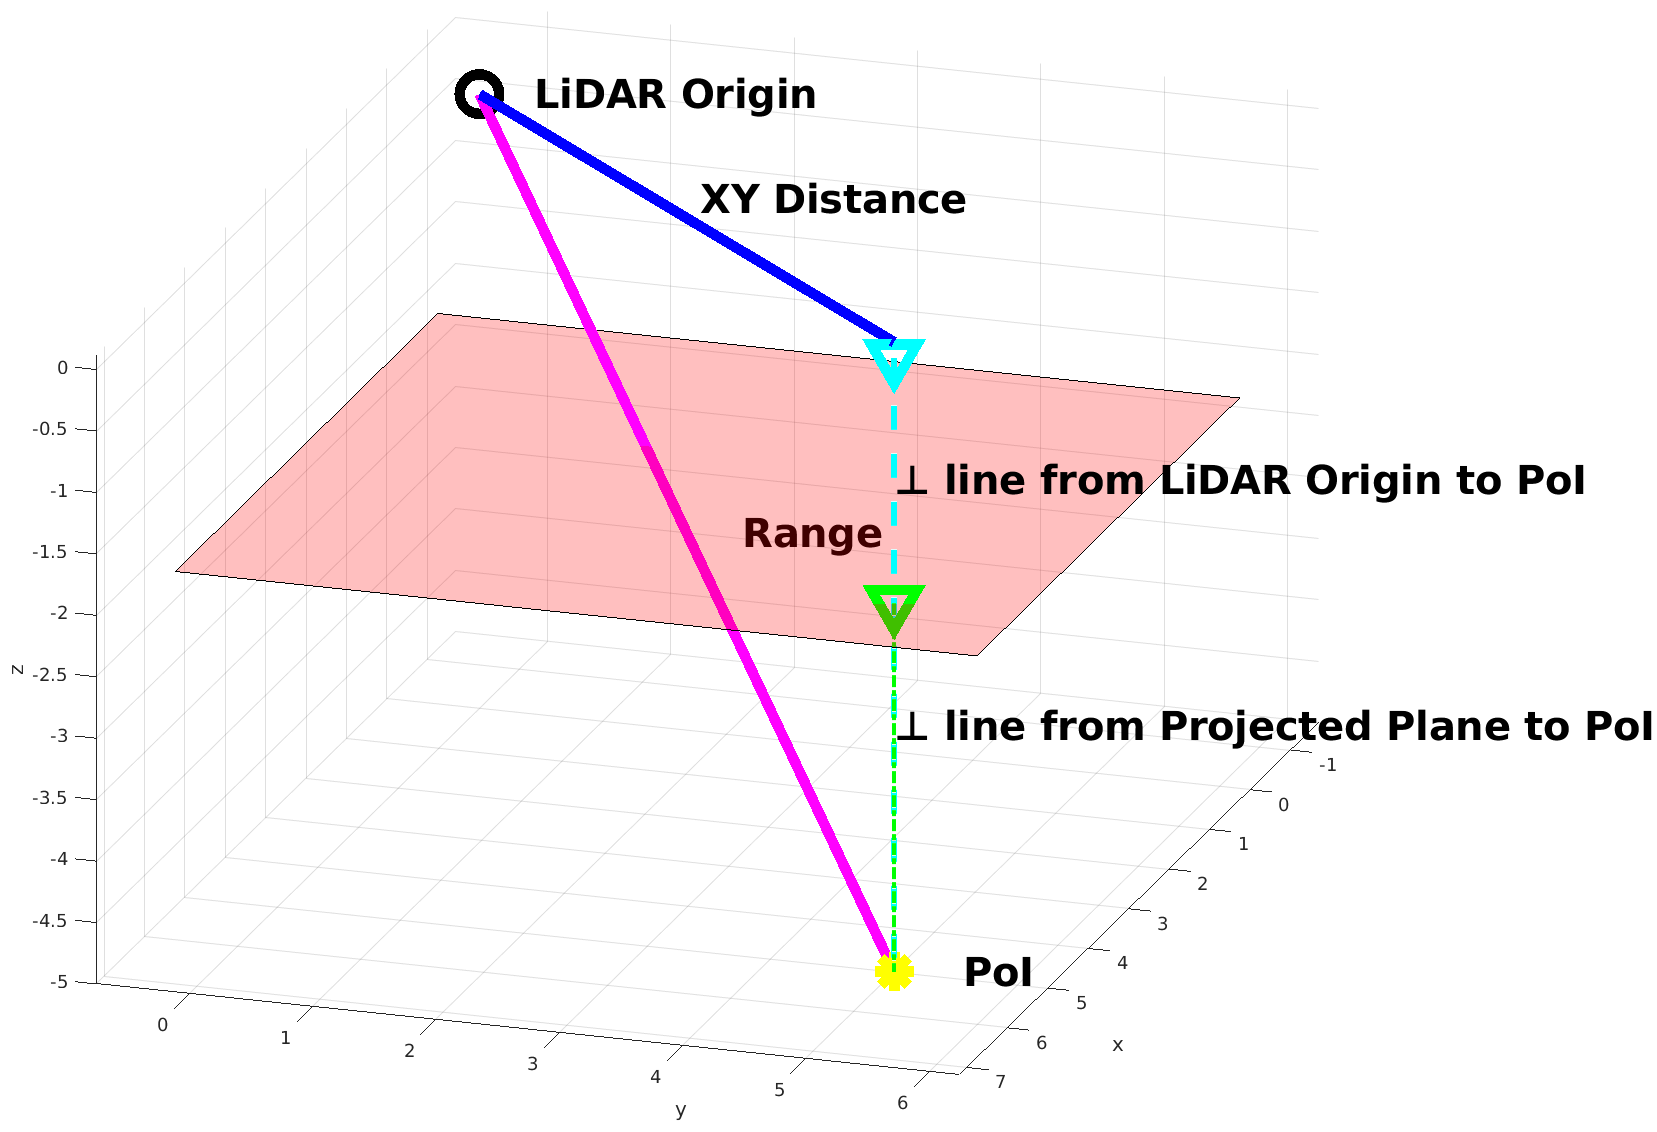
\includegraphics[width=1\linewidth]{Defense_Images/xy_vs_range}
			\caption[XY vs Range vs Z Height]{Three references for feature extraction may be seen in this simplified graph. First is the Range shown by the magenta line from the LiDAR origin to the Point of Interest (PoI). Second is the height from  LiDAR origin to the PoI (cyan). Finally, distance from the projected plane (red) to the PoI (green). XY Distance (blue) and Range (magenta) from the sensor was used consider the effect of distance from LiDAR origin to the PoI.}
			\label{fig:xy_vs_range}
		\end{figure}
	
		{Validation error was used as the primary means to compare RDF performance. MATLAB was used to load verification data and test increasing sizes of RDF algorithms for accuracy by comparing the known data types against the RDF result (Figure \ref{fig:moving_average_error_all}). RANSAC versus MLS was tested using identical feature sets (Figures \ref{fig:xyz_mls_comp_1} \ref{fig:xyz_mls_comp_2}). Validation error plots were used to influence feature sets and depth in later iterations of RDFs. Number of trees in the RDF verses error allowed for determination of an early stopping point for algorithm growth (Figure \ref{fig:early_stopping_xyz_100D}) by choosing the point where the change in moving average did not exceed 10\% and was within 15\% of the minimum error. Feature importance was calculated by counting the number of feature instances per RDF. Top twenty features of the algorithms that used all features (Figures \ref{fig:RAN_Top_Twenty_Histogram}, \ref{fig:MLS_Top_Twenty_Histogram}) were selected to compare testing accuracy. }
		
		\begin{figure}[H]
			\centering
			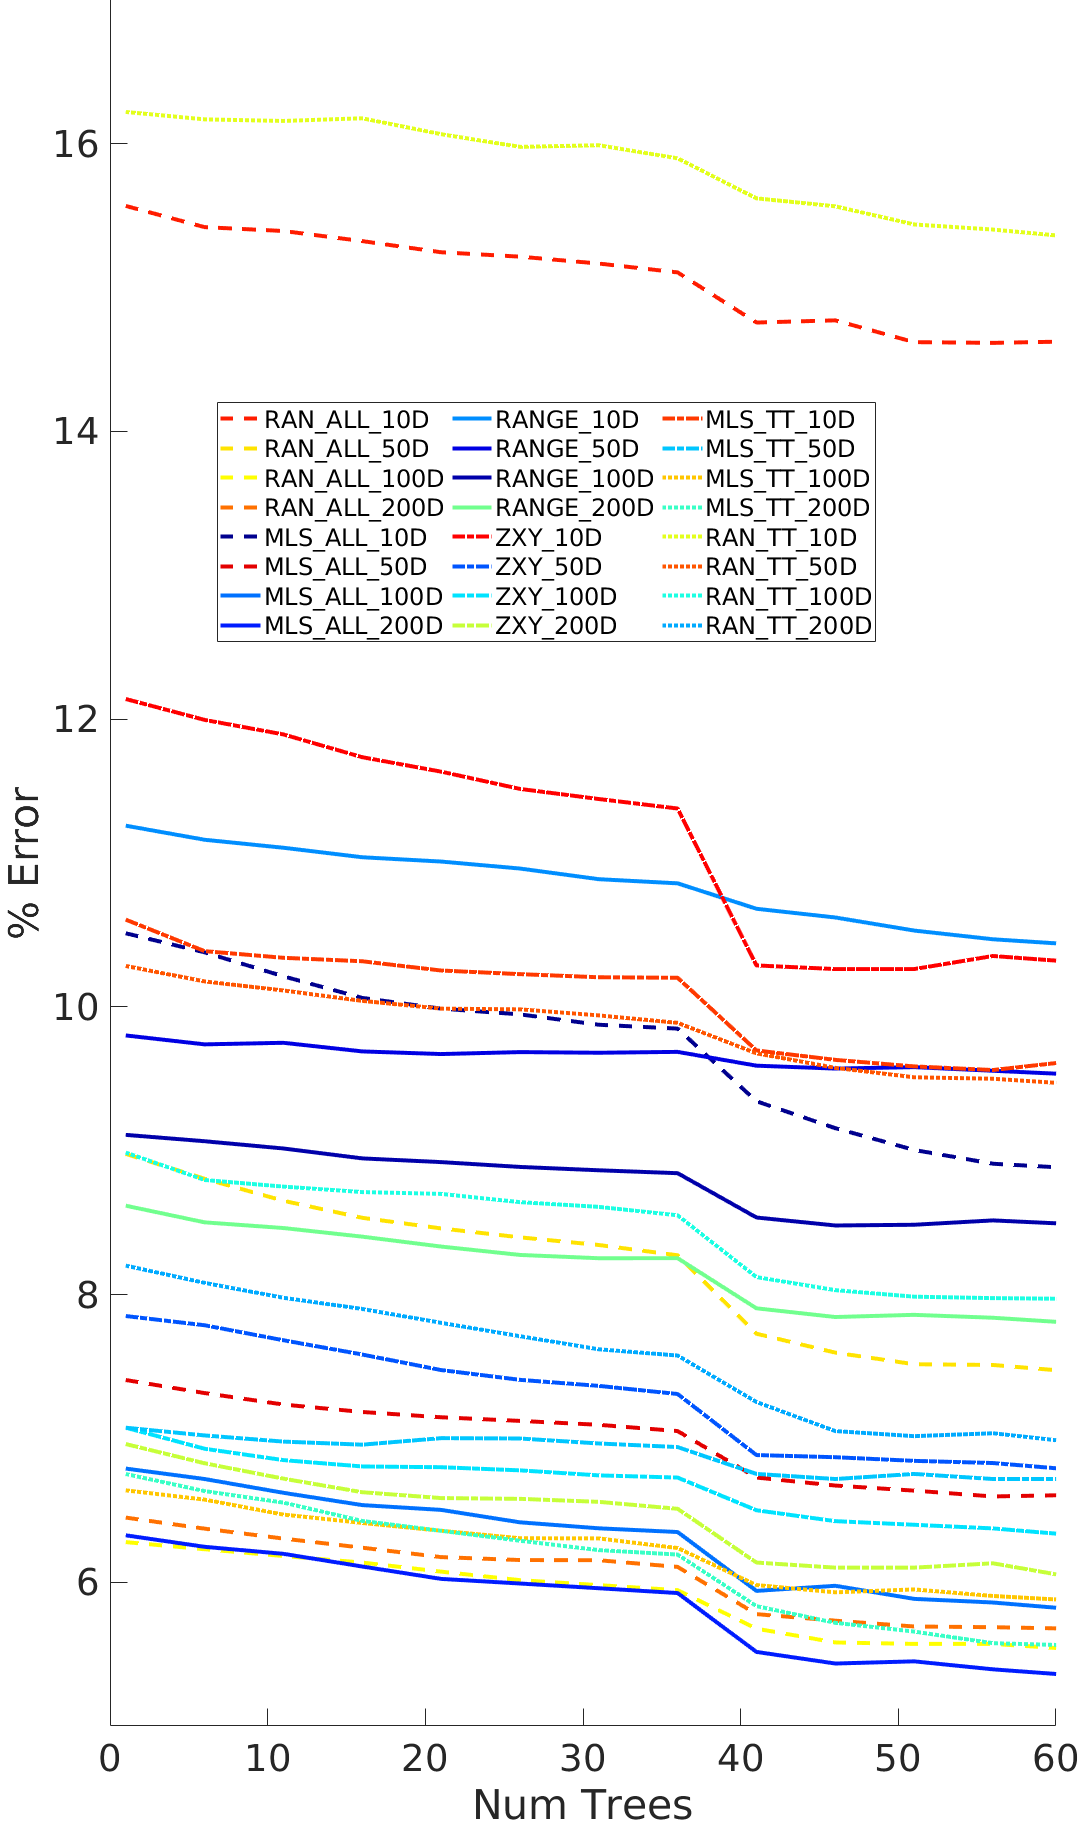
\includegraphics[width=0.7\linewidth]{Defense_Images/All_Vali_Error_3}
			\caption[Validation Error vs RDF Size]{Validation error verses size of the RDF. RDFs with the lowest validation error were chosen for further testing. Minimum validation error was achieved with the RDF that used X, Y, and Z components were used without range calculations with a maximum depth of 100 binary splits.}
			\label{fig:moving_average_error_all}
		\end{figure}
	
		\begin{figure}[H]
			\centering
			\begin{subfigure}{0.45\textwidth}
				\centering
				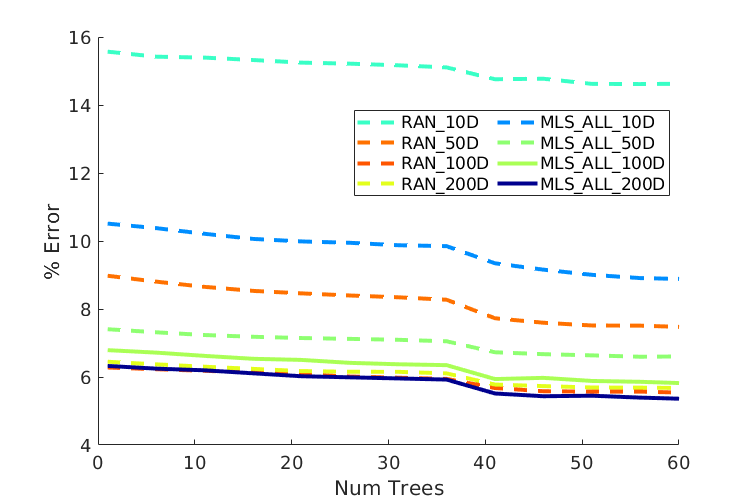
\includegraphics[width=1\linewidth]{Defense_Images/MLS_RAN_ALL}
				\caption[]{}
				\label{fig:all_mls_ransac_comp}
			\end{subfigure}
			\begin{subfigure}{0.45\textwidth}
				\centering
				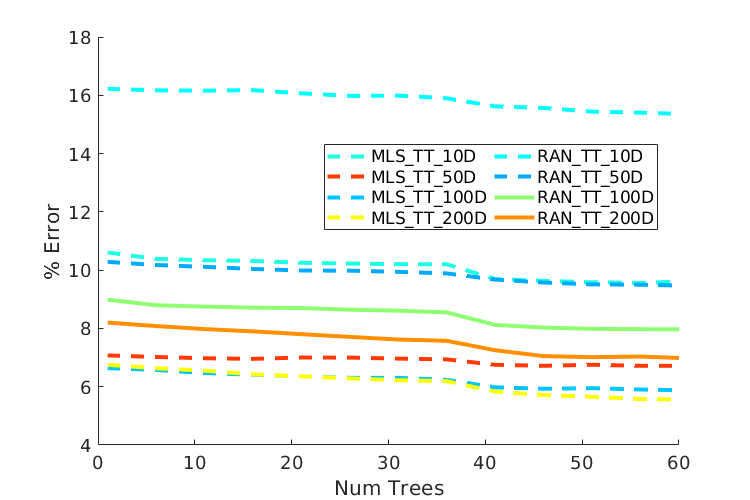
\includegraphics[width=1\linewidth]{Defense_Images/MLS_RAN_TT}
				\caption[]{}
				\label{fig:xyz_mls_ransac_comp}
			\end{subfigure}
			\caption[MLS vs RANSAC Validation Accuracy (1)]{MLS and RANSAC validation accuracy directly compared. All features are considered (a); Top 20 features used in (a) only (b).}
			\label{fig:xyz_mls_comp_1}
		\end{figure}
	
		\begin{figure}[H]
			\centering
			\begin{subfigure}{0.45\textwidth}
				\centering
				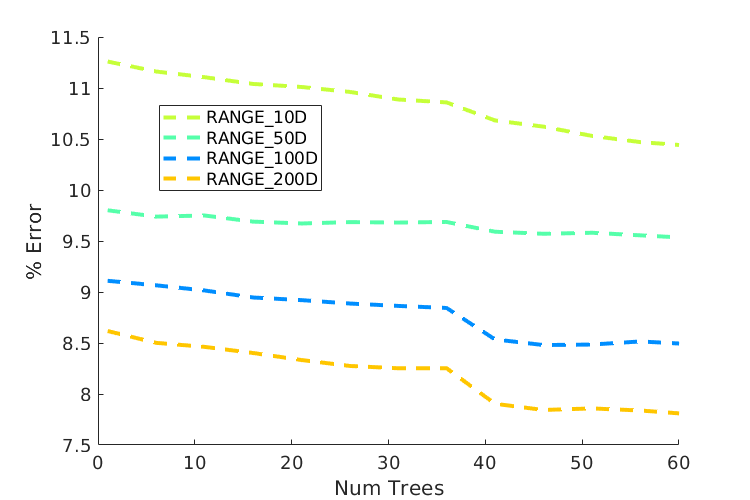
\includegraphics[width=1\linewidth]{Defense_Images/Range_Vali_Error}
				\caption[]{}
				\label{fig:range_mls_ransac_comp}
			\end{subfigure}
			\begin{subfigure}{0.45\textwidth}
				\centering
				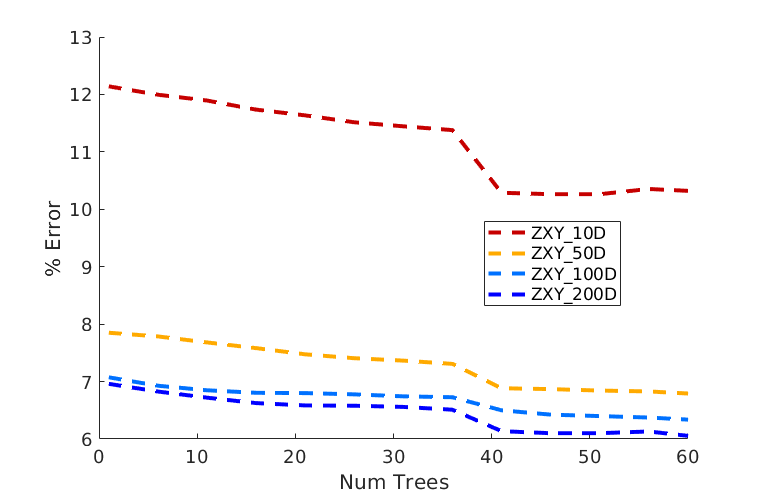
\includegraphics[width=1\linewidth]{Defense_Images/ZXY}
				\caption[]{}
				\label{fig:t20_mls_ransac_comp}
			\end{subfigure}
			\caption[MLS vs RANSAC Validation Accuracy (1)]{MLS and RANSAC validation accuracy directly compared. Range was used without X, Y, and Z components broken out (a); Plane projection not considered in (b), reference plane set as the LiDAR origin point.}
			\label{fig:xyz_mls_comp_2}
		\end{figure}

		\begin{figure}[H]
			\centering
			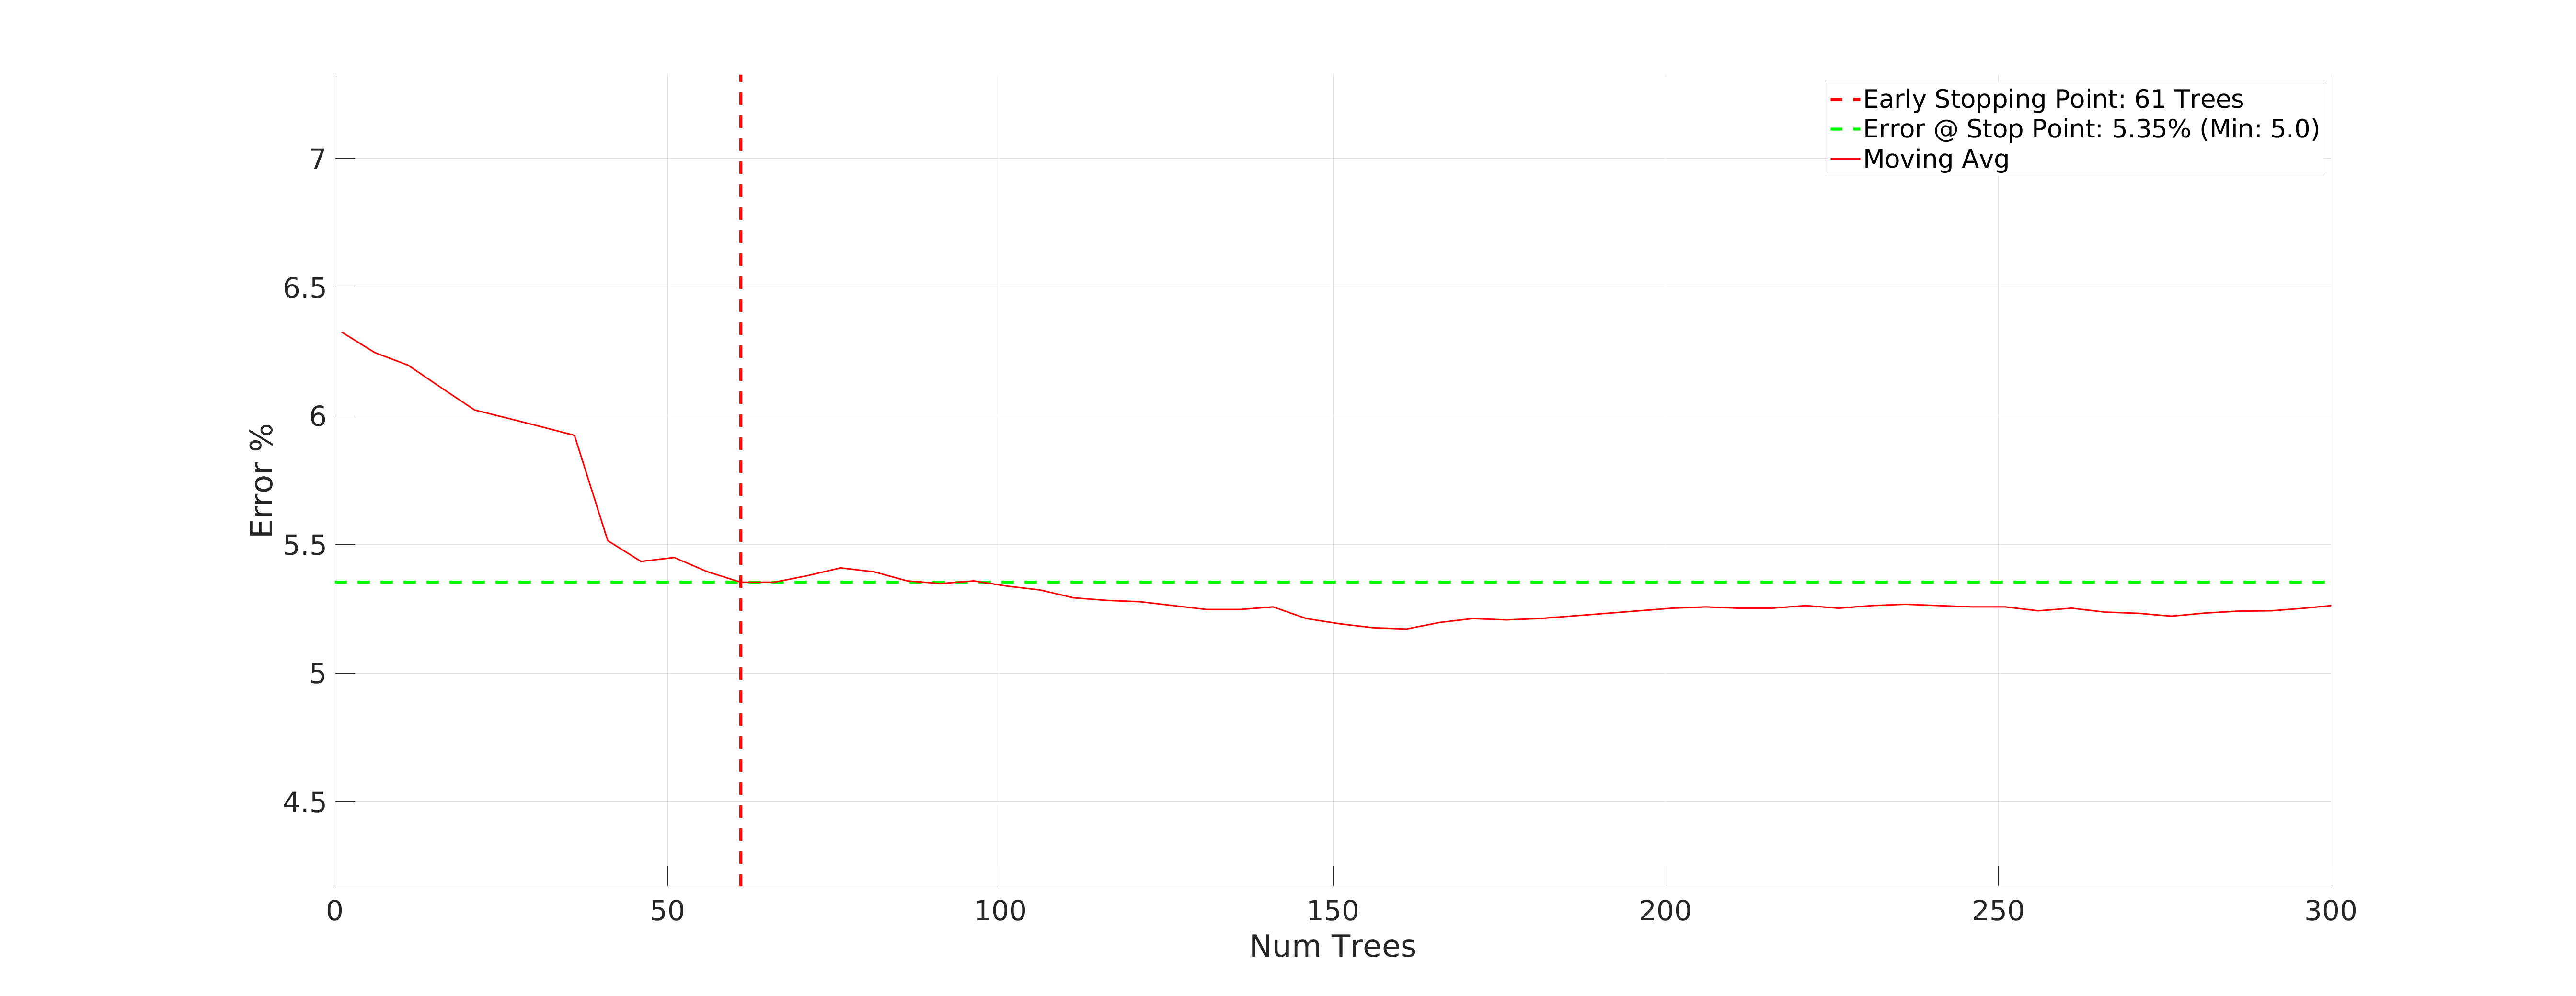
\includegraphics[width=1\linewidth]{Defense_Images/MLS_200D_early_stopping}
			\caption[Early Stopping]{Early stopping was be determined choosing the point where the change in the moving average did not exede 15\% and within 15\% of the minimum error. Plot shown is the RDF that yielded the lowest error in Figure \ref{fig:moving_average_error_all}.}
			\label{fig:early_stopping_xyz_100D}
		\end{figure}
	
%		{Verification tables were used to gauge RDF performance by comparing per-terrain type classification accuracy.  It was found that an average accuracy of 78.5\% may be achieved using the principal RDF used in this work (Table \ref{tab:Verification_Results}). Feature importance (Figure \ref{fig:Top_Ten_Histogram}) may be calculated by counting the number of feature instances per RDF. Feature types used in RDF creation may then be changed based on the usage. RDF were tested to determine the effect of feature inclusion or exclusion (Figure \ref{fig:err_sub_plot}). It was found that RDFs with large feature sets consistently produced more accurate results, and attempts at lowering the number of features consistently lowered accuracy (BACKUP WITH SOME PLOTS YA KNUCKLEHEAD). Therefore, RDFs with large feature sets were used for this work, however future work may include further research into lowering the number of required features. Number of trees in the RDF algorithm may increase accuracy at the cost of computational load, therefore RDFs with increasing number of trees were created and tested to determine the point of diminishing return. It was found that an RDF with X trees achieved Y\% accuracy.}
		
%		\begin{table}
%			\centering
%			\begin{tabular}{lc|c|c|c|c|}
%				\multicolumn{1}{c}{}       & \multicolumn{1}{c}{} & \multicolumn{4}{c}{Actual}                                                                                           \\
%				\multicolumn{1}{c}{}       & \multicolumn{1}{c}{} & \multicolumn{1}{c}{Gravel} & \multicolumn{1}{c}{Chipseal} & \multicolumn{1}{c}{Foliage} & \multicolumn{1}{c}{Grass}  \\ 
%				\cline{3-6}
%				\multirow{4}{*}{\rotatebox[origin=c]{90}{Predicted}} 	& Gravel 	& 93\% 		& 27\% 		& 0\% 		& 35\% \\ 
%																		\cline{3-6}
%																		& Chipseal 	& 3\% 		& 67\% 		& 0\% 		& 9\% \\ 
%																		\cline{3-6}
%																		& Foliage 	& 0\% 		& 0\% 		& 100\% 	& 7\% \\ 
%																		\cline{3-6}
%																		& Grass 	& 4\% 		& 16\% 		& 0\% 		& 54\% \\
%																		\cline{3-6}
%			\end{tabular}
%			\caption{Verification accuracy table for the principal RDF used for this work}
%			\label{tab:Verification_Results}
%		\end{table}
		
		\begin{figure}[H]
			\centering
			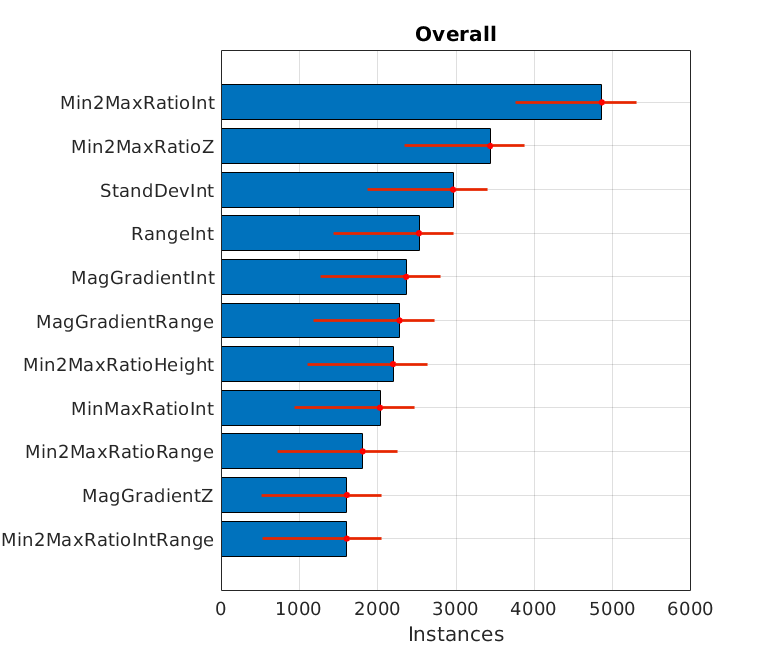
\includegraphics[width=0.7\linewidth]{Defense_Images/Top_Ten_Histogram}
			\caption[Example Feature Importance]{Feature importance may be determined by counting the number of instances of each feature per RDF. This histograms shows the top ten features used in an RDF that used all available features. Red bars indicate the ratio of true (right) and false (left) positives for road surfaces. Road surfaces are defined as data that has been classified as chipseal or gravel. }
			\label{fig:RAN_Top_Ten_Histogram}
		\end{figure}
	
		{Six Random Decision Forests were considered based on validation accuracy with the following specifications.}
		
		\begin{itemize}[itemsep=1pt]
			\item MLS (all features), 200 Depth, 61 Trees (Figure \ref{fig:mls_all_error_plots})
			\item RANSAC (all features), 100 Depth, 46 Trees (Figure \ref{fig:ran_all_error_plots})
			\item RANSAC (top twenty features), 100 Depth, 51 Trees (Figure \ref{fig:ran_tt_error_plots})
			\item MLS (top twenty features), 40 Depth, 41 Trees (Figure \ref{fig:mls_tt_error_plots})
			\item ZXY, 50 Depth, 41 Trees (Figure \ref{fig:zxy_error_plots})
			\item Range, 50 Depth, 51 Trees (Figure \ref{fig:range_error_plots})
		\end{itemize}
		
%		\begin{figure}[H]
%			\centering
%			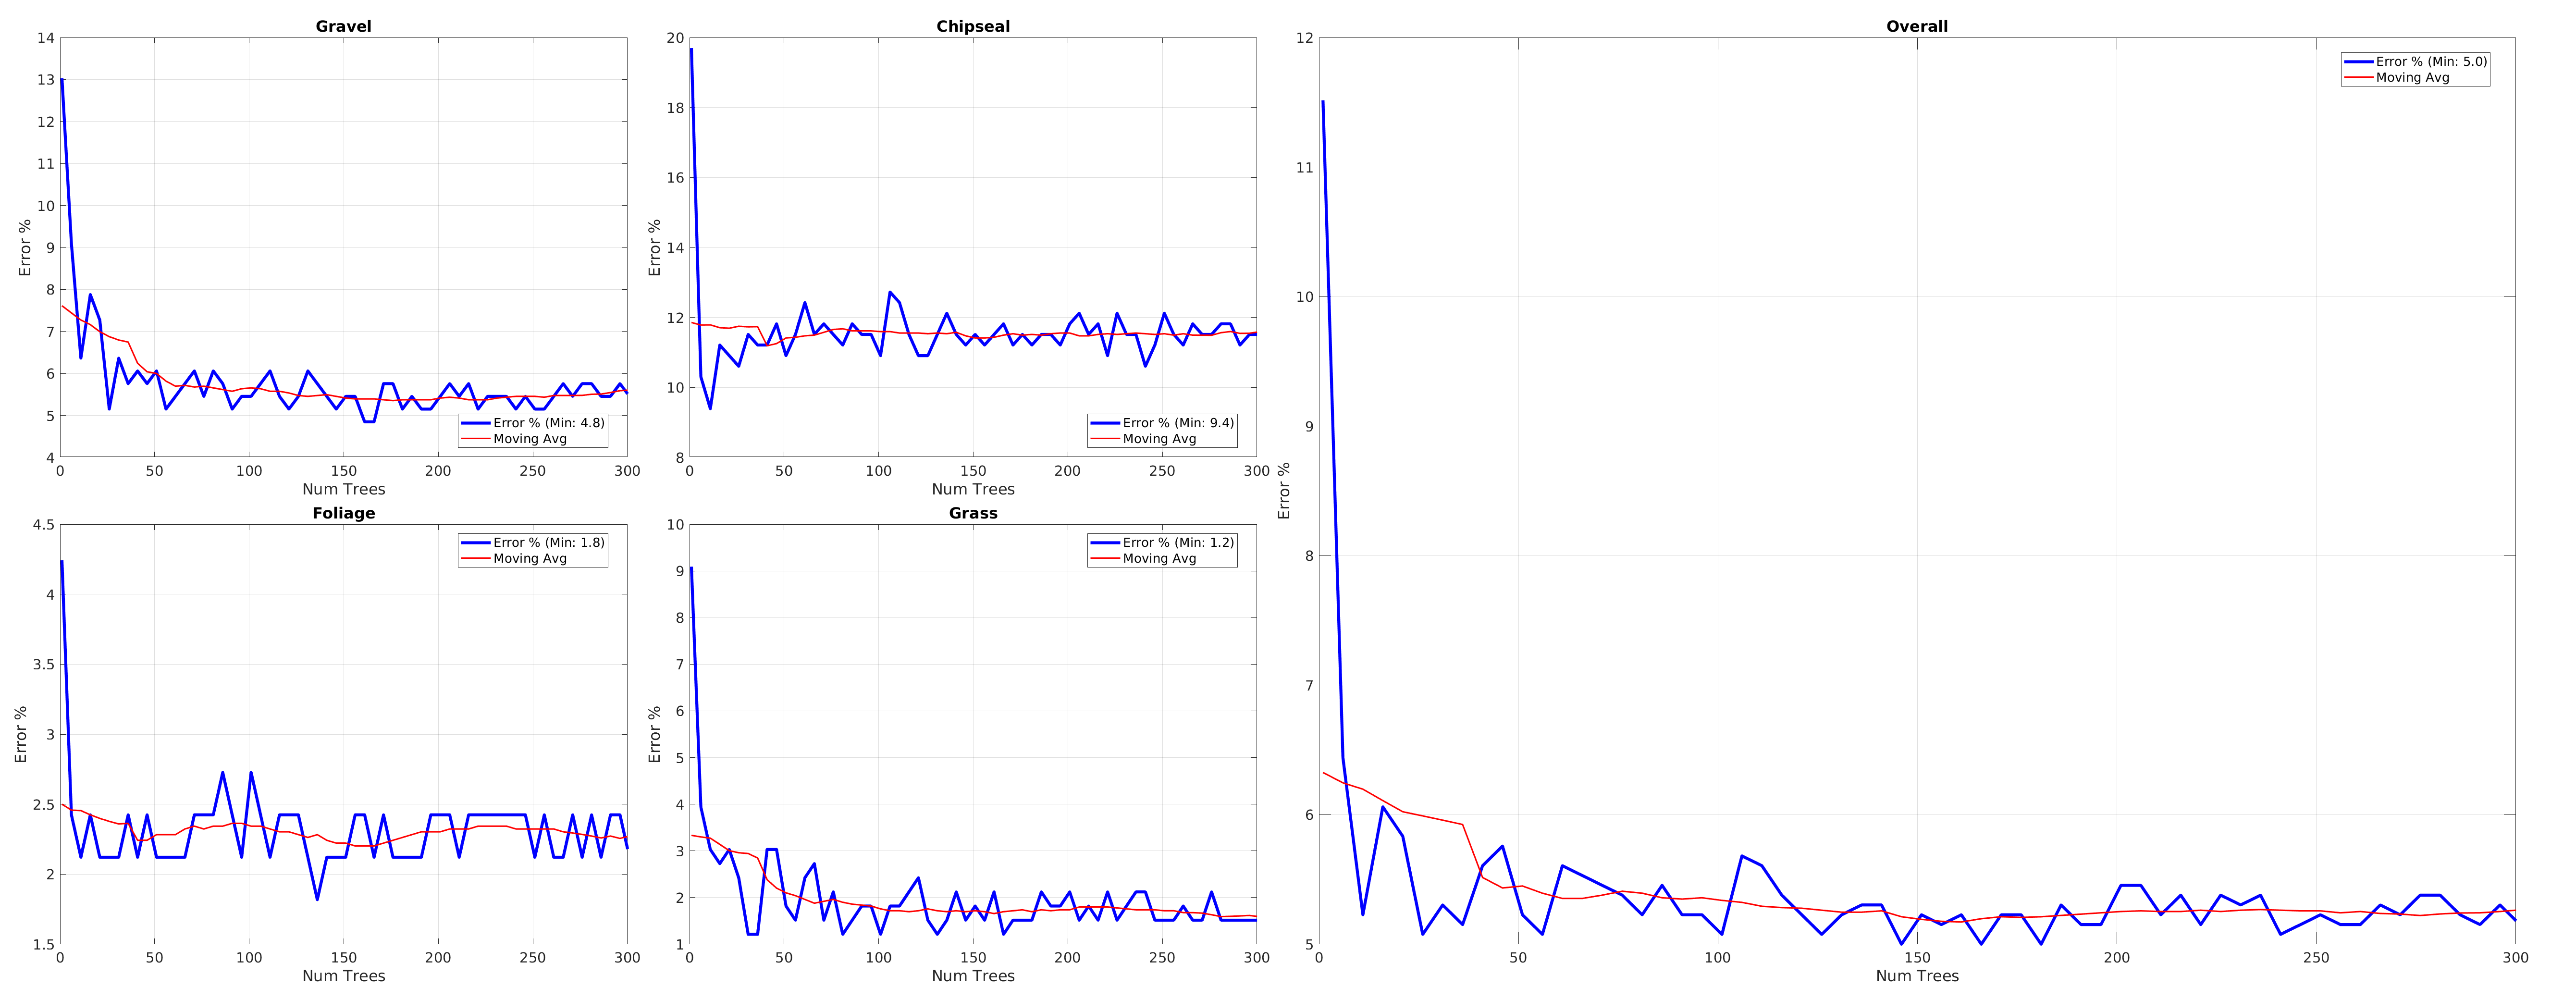
\includegraphics[width=1\linewidth]{Defense_Images/MLS_ALL_200D_err_sub_plot}
%			\caption[MLS All Error Plot]{Accuracy vs number of trees (blue) and moving average (red) shows diminishing returns as number of trees increases.}
%			\label{fig:err_sub_plot}
%		\end{figure}
%	
%		\begin{figure}[H]
%			\centering
%			\includegraphics[width=1\linewidth]{Defense_Images/MLS_ALL_200D_false_pos_neg_sub_plot}
%			\caption[MLS All False Positive/Negative]{False positive/negative detection of a road surface (gravel or chipseal). }
%			\label{fig:false_pos_neg_sub_plot}
%		\end{figure}
	
		\begin{figure}[H]
		
			\subfloat[]{%
				\includegraphics[clip,width=1.0\columnwidth]{Defense_Images/MLS_ALL_200D_err_sub_plot}
			}
			
			\subfloat[]{%
				\includegraphics[width=1.0\columnwidth]{Defense_Images/MLS_ALL_200D_false_pos_neg_sub_plot}
			}
		
			\subfloat[]{%
				\includegraphics[width=1.0\columnwidth]{Defense_Images/MLS_ALL_200D_early_stopping}
			}
			
			\caption[MLS All Error Plots]{MLS - All Features: Error Plots (a), False positive/negative identification of a road surface (gravel or chipseal) (b), Early stopping (c).}
			
			\label{fig:mls_all_error_plots}
			
		\end{figure}
	
		\begin{figure}[H]
			
			\subfloat[]{%
				\includegraphics[clip,width=1.0\columnwidth]{Defense_Images/ran_all_err_sub_plot}
			}
			
			\subfloat[]{%
				\includegraphics[width=1.0\columnwidth]{Defense_Images/ran_all_false_pos_neg_sub_plot}
			}
			
			\subfloat[]{%
				\includegraphics[width=1.0\columnwidth]{Defense_Images/ran_all_early_stopping}
			}
			
			\caption[RAN All Error Plots]{RANSAC - All Features: Error Plots (a), False positive/negative identification of a road surface (gravel or chipseal) (b), Early stopping (c).}
			
			\label{fig:ran_all_error_plots}
			
		\end{figure}

		\begin{figure}[H]
			
			\subfloat[]{%
				\includegraphics[clip,width=1.0\columnwidth]{Defense_Images/mls_tt_err_sub_plot}
			}
			
			\subfloat[]{%
				\includegraphics[width=1.0\columnwidth]{Defense_Images/mls_tt_false_pos_neg_sub_plot}
			}
			
			\subfloat[]{%
				\includegraphics[width=1.0\columnwidth]{Defense_Images/mls_tt_second_early_stopping}
			}
			
			\caption[MLS Top Twenty Error Plots]{MLS - Top Twenty: Error Plots (a), False positive/negative identification of a road surface (gravel or chipseal) (b), Early stopping (c).}
			
			\label{fig:mls_tt_error_plots}
			
		\end{figure}		
				
		\begin{figure}[H]
			
			\subfloat[]{%
				\includegraphics[clip,width=1.0\columnwidth]{Defense_Images/ran_tt_err_sub_plot}
			}
			
			\subfloat[]{%
				\includegraphics[width=1.0\columnwidth]{Defense_Images/ran_tt_false_pos_neg_sub_plot}
			}
			
			\subfloat[]{%
				\includegraphics[width=1.0\columnwidth]{Defense_Images/ran_tt_second_early_stopping}
			}
			
			\caption[RANSAC Top Twenty Error Plots]{RANSAC - Top Twenty: Error Plots (a), False positive/negative identification of a road surface (gravel or chipseal) (b), Early stopping (c).}
			
			\label{fig:ran_tt_error_plots}
			
		\end{figure}
	
		\begin{figure}[H]
			
			\subfloat[]{%
				\includegraphics[clip,width=1.0\columnwidth]{Defense_Images/mls_zxyt_err_sub_plot}
			}
			
			\subfloat[]{%
				\includegraphics[width=1.0\columnwidth]{Defense_Images/mls_zyx_false_pos_neg_sub_plot}
			}
			
			\subfloat[]{%
				\includegraphics[width=1.0\columnwidth]{Defense_Images/mls_zxy_early_stopping_exp}
			}
			
			\caption[ZXY Error Plots]{ZXY: Error Plots (a), False positive/negative identification of a road surface (gravel or chipseal) (b), Early stopping (c).}
			
			\label{fig:zxy_error_plots}
			
		\end{figure}
	
		\begin{figure}[H]
			
			\subfloat[]{%
				\includegraphics[clip,width=1.0\columnwidth]{Defense_Images/range_err_sub_plot}
			}
			
			\subfloat[]{%
				\includegraphics[width=1.0\columnwidth]{Defense_Images/range_false_pos_neg_sub_plot}
			}
			
			\subfloat[]{%
				\includegraphics[width=1.0\columnwidth]{Defense_Images/range_second_early_stopping}
			}
			
			\caption[Range Error Plots]{Range: Error Plots (a), False positive/negative identification of a road surface (gravel or chipseal) (b), Early stopping (c).}
			
			\label{fig:range_error_plots}
			
		\end{figure}
		
	
%		{Method of Least Squares plane projection was shown to be more efficient than RANSAC (1.408 ms for MLS and 4.888 ms for RANSAC, Figure \ref{fig:RANSAC_vs_MLL}), however it was found that RDFs created using MLS tended to be inaccurate (Figure \ref{fig:err_sub_plot_MLS}). For this reason, RANSAC was chosen as the plane projection method. Future work is needed to determine how to increase RDF accuracy using MLS as the plane projection method.}
%		
%		\begin{figure}[H]
%			\centering
%			\includegraphics[width=1\linewidth]{Defense_Images/err_sub_plot_MLS}
%			\caption[Accuracy vs Number of Trees - MLS]{Accuracy vs number of trees (blue) and moving average (red) shows increasing error using MLS as the plane projection method.}
%			\label{fig:err_sub_plot_MLS}
%		\end{figure}
		
	\section{Classifying Consecutive Scanning LiDAR}
	
		{Testing consecutive scans was completed by post processing rosbags that contained scanning LiDAR, GPS, and IMU data of an unmarked road, such as Sturbois Road near Athens Ohio (Figure \ref{fig:sturbois_1_Curve_camera}). Physical distance between the GPS, IMU, and LiDAR were rectified by measuring the distance between the modules. Rotational reference frames between the GPS, IMU, and LiDAR were rectified by applying appropriate rotational matrices. Transformation matrices were created by considering the GPS position and the IMU's roll, pitch, and yaw data. Point cloud data was then classified using the RDF derived in Objective I. Translation and rotation was applied to the terrain classification results with the closest matching transformation matrices (Figure \ref{fig:Classified_PointCloud_1_ALL}). Comparing averaged X, Y, and Z coordinates of classified quadrant (Figure \ref{fig:Classified_PointCloud_1_AVG}) allowed for easier comparison and scoring of the RDF classification to the manually classified areas. Consecutive scanning LiDAR data was compiled allowing for manually assigning areas representing road or side of road surfaces (Figure \ref{fig:Manually_Classified_Areas}). Side of road area were manually defined as an area roughly one meter outwards from the road edge for consideration of road edge detection. Per-Quadrant classification rate data was gathered and plotted, the average rate being 2.97 quadrants per second (Figure \ref{fig:Time_Hz_Rate}). This was tested with a machine with 64 GB of DDR4 RAM and a Ryzen 9 5900X 12 core x 24 thread CPU.}
		
		{Six stretches of unmarked gravel and chipseal roads were considered for detection accuracy.}
		
		\begin{itemize}[itemindent=1px]
			\item 
		\end{itemize}
		
		\begin{figure}[H]
			\centering
			\includegraphics[width=1.0\linewidth]{Defense_Images/sturbois_1_Curve_camera}
			\caption[Sturbois Road Curve]{A Curved portion of Sturbois Road.}
			\label{fig:sturbois_1_Curve_camera}
		\end{figure}
		
		\begin{figure}[H]
			\centering
			\begin{subfigure}{0.49\textwidth}
				\centering
				\includegraphics[width = \textwidth]{Defense_Images/sturbois_curve_1_all_classified.png}
				\caption{All}
				\label{fig:Classified_PointCloud_1_ALL}
			\end{subfigure}
			\begin{subfigure}{0.49\textwidth}
				\centering
				\includegraphics[width = \textwidth]{Defense_Images/sturbois_curve_1_avg_classified.png}
				\caption{Averaged}
				\label{fig:Classified_PointCloud_1_AVG}
			\end{subfigure}
			\caption[Compiled Classified Point Cloud]{Sturbois Rd., curved section classified and combined point clouds. (a) Shows the all points. (b) Shows the averaged x,y,z coordinates per classified quadrant.}
			\label{fig:Combined_Classified_Clouds_1}
		\end{figure}
	
		\begin{figure}[H]
			\centering
			\includegraphics[width=0.7\linewidth]{Defense_Images/sturbois_curve_1_manual_classified.png}
			\caption[Manually Classified Areas - Sturbois Curved Section]{Curved portion from Sturbois Rd. is manually classified by road terrain type. Side of road is considered for road edge detection.}
			\label{fig:Manually_Classified_Areas}
		\end{figure}
	
		\begin{figure}[H]
			\centering
			\includegraphics[width=1\linewidth]{Defense_Images/Time_Hz_Rate.png}
			\caption[Quadrant Classification Rate]{Per-quadrant classification rate is shown here in Hz. Average rate is 2.97 Hz.}
			\label{fig:Time_Hz_Rate}
		\end{figure}
	
		{Quadrant size affects terrain classification accuracy at the expense of granularity of results and computational time. Smaller quadrants allow for greater resolution of terrain classification, however more computational time is required. Larger quadrants allow for swifter classification, however as consecutive scanning LiDAR points may include road and non-road surfaces, classification accuracy may suffer. Future work may include optimizing quadrant size, however for the purpose of this work, one hundred quadrants per channel (approx. 35 points per quadrant) yielded acceptable results.}
	
	\section{Consecutive Scanning LiDAR Classification Results}
	
		{Manually classified areas were projected over the classified point cloud made of averaged quadrant coordinates from a curved portion of Sturbois Road (Figure \ref{fig:both_classification_things_sturbois_curve_1}). Sturbois Road consists of gravel that is smaller than that used in the training data, and features a strip of grass down the center of the one-lane road (Figure \ref{fig:sturbois_1_Curve_camera}). Classification accuracy of the road surface was calculated and side-of-road classification results were found. It was found that the road terrain type was correctly identified at a 79.3\% accuracy rate, with a true-positive rate of 81.3\% for road surface detection which includes both gravel and chipseal identifications. False negative detection of a road surface was below 20\%. Side-of-road areas had a distinct drop off of positive road identification with X\%, and an increase of negative road identification with Y\%.} 
		
		\begin{figure}[H]
			\centering
			\includegraphics[width=0.7\linewidth]{Defense_Images/both_classification_things_sturbois_curve_1}
			\caption[On-Road Classification Results 1]{Average X, Y, and Z coordinates of classified points are shown lying on manually defined road surfaces.}
			\label{fig:both_classification_things_sturbois_curve_1}
		\end{figure}
	
		\begin{table}[H]
			\centering
			\begin{tabular}{lll}
							& Road 		& Side-of-Road 	\\
				Gravel   	& 79.3\% 	& 0\%			\\
				Chipseal 	& 2.0\% 	& 0\%  			\\
				Foliage  	& 11.2\% 	& 0\% 			\\
				Grass    	& 7.5\% 	& 0\%
			\end{tabular}
			\caption[Sturbois Road Curve Example 1]{Accuracy for Sturbois Road and Side-of-Road analysis}
			\label{tab:Sturbois_Curve_1_Road_Results}
		\end{table}
	
		{Repeat above for several completed examples.}
		
} % End Results


\chapter{Conclusion}
{
	
	{The proposed work addresses the problem of road surface detection on unmarked gravel and chipseal roads. Current LiDAR and Camera based detection models are insufficient due to lack of distinct features typical of urban roads, such as painted line markings or curbs, or have excessive computational or storage requirements. The completed work balanced accuracy and efficiency by using less intensive analysis techniques of smaller point cloud data sets. The first objective was to determine a method of detecting an unmarked gravel road. The second objective was to evaluate performance of road detection along stretches of unmarked gravel and chipseal roads. The final deliverable of the completed work was a method of detecting physical unmarked gravel and chipseal roads by using a terrain classification approach to predicting road surface area. The impact of this work is that autonomous vehicles using LiDAR may be able to detect gravel road surfaces in real time, allowing autonomous operations on 1.5 million miles of previously undetected rural roads.}

}


\appendix

\chapter{Source Code}{
	
	\section{Additional Tables}{
	
	
	
	}
	
	\section{MATLAB Source Code}{
		
%			\lstinputlisting[style=Matlab-editor, basicstyle=\mlttfamily\scriptsize, caption={PCD STACK CLASSIFIER}]{PCD_STACK_CLASSIFIER_DEFENSE_THING.m}
%			\lstinputlisting[style=Matlab-editor, basicstyle=\mlttfamily\scriptsize, caption={Grabbing Transformation Matrix}]{get_tform.m}
%			\lstinputlisting[style=Matlab-editor, basicstyle=\mlttfamily\scriptsize, caption={Making Combined Point Cloud}]{make_combined_pcd.m}
%			\lstinputlisting[style=Matlab-editor, basicstyle=\mlttfamily\scriptsize, caption={Matching Timestamps}]{matchTimestamps.m}
%			\lstinputlisting[style=Matlab-editor, basicstyle=\mlttfamily\scriptsize, caption={Progress Bar}]{parfor_progress.m}	
		
	} % End Appendix Obj 1 T 2

} % End Chapter - Appendix Source Code

%
%%% The \references command marks the point where the bibliography will
%%% be inserted.  In the example below, the BibTeX commands are
%%% inserted into the macro definition, but one could also manually
%%% enter the bibliography entries if desired.
%\references{
%  %ETD does not define a particular required bibliography style.
%  %They DO require entries to end in a period UNLESS they end in a URL
%  %or DOI AND that DOIs be set in the same font as everything else.
%  %I have modified the alphaurl style file, to conform to these requirements.
%  
  \bibliographystyle{ieeetr}  
  \bibliography{resources.bib} 
%}

%%\appendix           % Indicates the transition from chapters to appendices.  
                    % Subsequent 

%%\chapter{An Appendix}
%%\section{A Section in the Appendix}

\end{document}
